% Stellar UV photons versus cosmic-ray electrons as reionization agents at z=10.
% Companion to photon_vs_electron.py and QUESTION_LOG.md.
% Every number is reproduced by:  python3 photon_vs_electron.py
% Gate:  python3 check_provenance.py photon_vs_electron.tex \
%           photon_vs_electron_results.json,yield_comparison_results.json,\
%           provenance/registry_z20.json photon_vs_electron.log
% The z=20 registry is built by make_z20_registry.py, which suffixes every key
% _z20 so the gate can hold both redshifts without a key meaning two things.
\documentclass[11pt,a4paper]{article}
\usepackage[margin=2.3cm]{geometry}
\usepackage{amsmath,amssymb,array,booktabs,graphicx,xcolor}
% Figures live in Images/ since the 2026-09-15 reorganisation. Both entries
% are listed so the document builds either from Text_files/ or from the root.
\graphicspath{{../Images/}{Images/}{./}}

\usepackage[colorlinks=true,linkcolor=black,citecolor=black,urlcolor=blue]{hyperref}
\usepackage{siunitx}
\DeclareSIUnit{\erg}{erg}
\newcommand{\ion}[2]{\textsc{#1\,\MakeLowercase{#2}}}
\newif\ifprovdraft
\provdrafttrue
\newcommand{\src}[1]{%
  \ifprovdraft
    \ifmmode{}^{\text{\color{gray}\scriptsize\texttt{#1}}}%
    \else{\color{gray}\scriptsize$^{\texttt{#1}}$}%
    \fi
  \fi}

\title{Stellar UV photons versus cosmic-ray electrons\\
\large as reionization agents in the $z=10$ intergalactic medium}
\author{Generated with an AI assistant, under the project Master Rules}
\date{Reproduced by \texttt{python3 photon\_vs\_electron.py}}

\begin{document}
\maketitle

\begin{abstract}
\noindent
We compare two candidate ionizing agents for the neutral IGM at $z=10$
($x_e = 10^{-4}$, pure H --- the scenario of the companion calculation): escaping
stellar Lyman-continuum photons, and cosmic-ray electrons accelerated by the
supernovae of the same stellar population. One star-formation history feeds both
channels, so the comparison is internally consistent. Using the JWST-measured UV
luminosity density of Donnan et al.~\cite{donnan24} and the ionizing efficiency of
Llerena et al.~\cite{llerena25}, and converting primary energy to ionizations with
the checked yield model of the companion work, we find
$\zeta_\gamma = 4.647\times10^{-18}$\src{zeta\_gamma\_s} and
$\zeta_e = 8.299\times10^{-22}$\src{zeta\_e\_s} ionizations per second per
hydrogen atom: stellar UV leads by a factor
$5599$\src{zeta\_ratio}. Because both channels are exactly linear in their own
normalisation, parity would require
$\epsilon_{\rm CR}f_e = 5.6$\src{eps\_cr\_fe\_crossover} --- more energy in
cosmic-ray electrons than the supernova releases. \textbf{On these assumptions CR
electrons cannot reach parity at any physical acceleration efficiency}, in
independent agreement with Leite et al.~\cite{leite17}. In the standard
normalisation --- ionizations per atom per \emph{recombination} time, the clock
that decides whether ionization can be maintained (\cite{md14} eq.~24) --- we
find $\zeta_\gamma t_{\rm rec} = 0.06472$\src{zeta\_gamma\_trec} against
$\zeta_\gamma t_H = 0.1039$\src{zeta\_gamma\_tH} in the Hubble-time form, the two
differing by exactly $t_{\rm rec}/t_H = 0.6228$\src{t\_rec\_over\_t\_H}. Both sit
well below unity, and that is the physically correct answer: at $z=10$ escaping
stellar photons cannot yet balance recombinations, which is what an incomplete
reionization means. Keeping the IGM ionized needs
$2.606$\src{ion\_per\_atom\_needed\_per\_tH} ionizations per atom per Hubble
time, so the $z=10$ stellar rate falls short by
$25.1$\src{reion\_shortfall\_factor} and the cosmic-ray rate by
$1.404\times10^{5}$\src{reion\_shortfall\_factor\_CR} (\S\ref{sec:norm}).
\end{abstract}

\section{Assumptions}
Every choice marked SCANNED was made by the user and is logged, with the options
offered, in \texttt{QUESTION\_LOG.md}.
\begin{enumerate}\itemsep2pt
\item \textbf{Scenario} identical to the companion calculation: neutral IGM at
      $z=10$\src{z}, $x_e = 10^{-4}$\src{x\_e} held static, pure atomic hydrogen
      at the mean density $n_{\rm H} = \SI{2.529e-4}{\per\cubic\centi\metre}$\src{n\_H\_cm3}.
\item \textbf{UV luminosity density} $\log_{10}(\rho_{\rm UV}/\mathrm{erg\,s^{-1}
      Hz^{-1}cMpc^{-3}}) = 25.12$\src{log\_rho\_UV}, measured \emph{at} $z=10$
      \cite{donnan24}, with asymmetric error $+0.07/-0.08$~dex. SCANNED.
      \textbf{Truncated at the faint end.} This is the luminosity-weighted
      integral of the luminosity function down only to $M_{\rm UV}=-17$
      \cite{donnan24}, not the total UV luminosity density. It is therefore a
      \emph{lower bound}, and so is everything derived from it --- including
      $\rho_{\rm SFR}$ through the $K_{\rm UV}$ of \cite{md14} below, and hence
      both $\zeta_\gamma$ and $\zeta_e$. The competition ratio is unaffected,
      since $\rho_{\rm UV}$ cancels from it, but the reionization budget of
      \S\ref{sec:budget} is not.
\item \textbf{$\rho_{\rm UV}\to\rho_{\rm SFR}$} with
      $K_{\rm UV} = 1.15\times10^{-28}$\src{K\_UV}~$M_\odot\,\mathrm{yr^{-1}}/
      (\mathrm{erg\,s^{-1}Hz^{-1}})$ \cite{md14}. The Salpeter IMF is inherited
      from that conversion, and is then used consistently in the supernova rate.
\item \textbf{Ionizing efficiency} $\log_{10}(\xi_{\rm ion}/\mathrm{Hz\,erg^{-1}})
      = 25.28$\src{log\_xi\_ion} \cite{llerena25}, with the observed
      $0.42$\src{xi\_ion\_scatter\_dex}~dex scatter propagated.
\item \textbf{Escaping stellar spectrum.} The identified population is the
      one fitted to U37126, a star-forming galaxy at $z = 10.255$ --- our
      redshift --- by Marques-Chaves et al.~\cite{mc26}: BPASS v2.2.1,
      \texttt{imf135\_300}, $Z = 0.003$, constant star formation, age
      $6.8\pm1.6$~Myr, $\beta_{\rm UV} = -2.88\pm0.10$.
      \textbf{The BPASS spectrum itself could not be obtained} --- the tables are
      not reachable here and the paper quotes only $Q_{\rm H}$ --- so it is
      \emph{not} invented. The shape is carried by the standard parametrisation
      for reionization-era sources, $f_\nu\propto\nu^{-\alpha}$ across 1--4~Ryd
      (photon number $dN/dE\propto E^{-(\alpha+1)}$), with $\alpha$
      \emph{bracketed} over 1--3 rather than asserted. \S\ref{sec:sed} shows the
      conclusion does not depend on it. The $T_{\rm eff} =
      \SI{5e4}{\kelvin}$\src{T\_eff\_K} blackbody is retained as a comparison.
\item \textbf{Escape fraction} $f_{\rm esc}$ SCANNED; the canonical
      $0.10$\src{f\_esc\_fid} is a convention adopted to close photon budgets,
      \emph{not} a measurement. That is precisely why it is scanned.
\item \textbf{CR electrons} injected as $E^{-p}$ with
      $p = 2.2$\src{CR\_index}, between
      \SI{1e3}{\electronvolt}\src{CR\_E\_min\_eV} and
      \SI{1e12}{\electronvolt}\src{CR\_E\_max\_eV} (user's choice; index from
      \cite{leite17}).
\item \textbf{Supernovae}: $E_{\rm SN} = \SI{1e51}{\erg}$\src{E\_SN\_erg};
      $\epsilon_{\rm CR}\times f_e$ SCANNED with canonical
      $10^{-3}$\src{eps\_CR\_fe\_fid} from $\epsilon_{\rm CR}=0.1$ (diffusive
      shock acceleration) and $f_e = K_{ep} = 0.01$ (Galactic $e/p$ at 10~GeV).
\item \textbf{Electron yields} from \textbf{the loss+IC route}: \texttt{igm\_losses.py}
      --- adiabatic, synchrotron, inverse Compton with Klein--Nishina, Coulomb
      (Gould 1972), collisional excitation (Stone \& Kim 2002), collisional
      ionization (RBED, Kim et al.\ 2000) and bremsstrahlung --- with
      ionizations counted event by event, knock-on electrons followed through
      the BED secondary spectrum (Kim \& Rudd 1994), plus the IC-secondary
      photoionization channel. Model~C of the companion work, which drove the
      previous version of this paper, agrees to $7.7\%$ and is retained as the
      cross-check that validated this route.
\item \textbf{Every injected CR electron deposits in the IGM} --- no escape or
      confinement modelling. This \emph{favours} the CR channel, deliberately: if
      photons still win, the conclusion is robust.
\item \textbf{No recombinations, no clumping.} $\zeta$ is an ionization rate per
      atom, not a net reionization rate.
\end{enumerate}

\section{Derivation}
\subsection{Quantities derived here rather than adopted}
The supernova rate is obtained by integrating the Salpeter IMF, not by quoting a
number: with $\phi(m)\propto m^{-2.35}$ over $0.1$--$100\,M_\odot$ and
core-collapse progenitors above $8\,M_\odot$,
\begin{equation}
\frac{N_{\rm SN}}{M_\odot} = \frac{\int_{8}^{100} m^{-2.35}\,dm}
                                  {\int_{0.1}^{100} m^{-1.35}\,dm}
 = 7.422\times10^{-3}\src{sn\_per\_Msun},
\end{equation}
one supernova per $135\,M_\odot$ formed. This is verified symbolically in
\texttt{sympy} and again by quadrature. The mean energy of an injected electron,
\begin{equation}
\langle E\rangle = \frac{\int E^{1-p}dE}{\int E^{-p}dE}
 = \SI{5905}{\electronvolt}\src{mean\_injected\_E\_eV},
\end{equation}
is likewise closed-form, sympy-verified, and dominated by $E_{\rm min}$ because
$p>2$.

\subsection{The two channels}
\begin{align}
\dot n_\gamma &= f_{\rm esc}\,\xi_{\rm ion}\,\rho_{\rm UV}
   = 2.512\times10^{49}\src{ndot\_gamma\_cMpc3}\ \mathrm{s^{-1}cMpc^{-3}},\\
\dot R_{\rm SN} &= \rho_{\rm SFR}\,\frac{N_{\rm SN}}{M_\odot}
   = 3.565\times10^{-13}\src{R\_sn\_cMpc3\_s}\ \mathrm{s^{-1}cMpc^{-3}},\\
L_e &= \dot R_{\rm SN}\,(\epsilon_{\rm CR}f_e)\,E_{\rm SN}
   = 3.565\times10^{35}\src{L\_e\_erg\_s\_cMpc3}\ \mathrm{erg\,s^{-1}cMpc^{-3}},\\
\dot n_e &= L_e/\langle E\rangle
   = 3.769\times10^{43}\src{ndot\_e\_cMpc3}\ \mathrm{s^{-1}cMpc^{-3}}.
\end{align}
The differential emissivity of panel (a) is
$d\dot n/d\log_{10}E = \ln(10)\,E\,\dot n\,p(E)$ with $p$ the normalised
injection spectrum, and the ionization rate of panel (b) is
\begin{equation}
\boxed{\;\frac{d\zeta}{d\log_{10}E}
 = \frac{1}{n_{\rm H}}\,\frac{d\dot n}{d\log_{10}E}\,N_{\rm ion}(E)\;}
\end{equation}
with $N_{\rm ion}$ the checked yield of the companion work. Both $\dot n$ and
$n_{\rm H}$ scale as $(1+z)^3$, so $\zeta$ is independent of the
comoving/proper convention; that cancellation is checked numerically rather than
asserted.

\section{Verification}
\texttt{photon\_vs\_electron.py} runs 16 checks; all pass.

\begin{table}[h]\centering\small
\begin{tabular}{@{}llp{8.0cm}@{}}
\toprule
ID & Check & Outcome \\
\midrule
C25 & \texttt{sympy} on the IMF integral & symbolic, closed-form and quadrature agree to $10^{-12}$ \\
C25 & \texttt{sympy} on $\langle E\rangle$ & symbolic vs closed form to $10^{-10}$ \\
C28 & both spectra are pdfs & integrate to 1; the electron one \emph{in $\ln E$} --- in linear space the same \texttt{quad} returns $-10^{-10}$ over nine decades \\
C29 & CR injection two ways & $L_e/\langle E\rangle$ vs $\dot R_{\rm SN}\times$(electrons per SN), exact \\
C26 & comoving/proper invariance & the factor $1331$ cancels to $10^{-12}$ \\
C31 & $\zeta_e$ two quadratures & trapezoid vs adaptive \texttt{quad} \\
C30 & \textbf{pre-registered} order of magnitude & 2--4 decades predicted in \texttt{QUESTION\_LOG.md} \emph{before} the code existed; found $3.75$\src{zeta\_ratio\_decades} \\
C32 & \cite{md14} eq.~(24) reproduced & $t_{\rm rec} = 3.149$\src{t\_rec\_z6\_C1\_Gyr}~Gyr at $(1+z)/7=1$, $C_{\rm IGM}=1$ vs their 3.2~Gyr; $t_{\rm rec}/t_H = 0.6228$\src{t\_rec\_over\_t\_H} vs their ``$\sim$60\%'' \\
C33 & maintenance criterion & $\zeta_\gamma t_{\rm rec} = 0.06472$\src{zeta\_gamma\_trec} $< 1$: recombinations win at $z=10$, as they must \\
C34 & shortfall stated, not hidden & requirement $2.606$\src{ion\_per\_atom\_needed\_per\_tH} per $t_H$; stellar short by $25.1$\src{reion\_shortfall\_factor}, CR by $1.404\times10^{5}$\src{reion\_shortfall\_factor\_CR} \\
C18 & deliberate failure & the yield model moves the CR channel by $>10\times$, so quoting it without naming the model would be meaningless \\
C26 & linearity and the crossover & exact to $10^{-10}$, giving $\epsilon_{\rm CR}f_e = 5.6$\src{eps\_cr\_fe\_crossover} for parity \\
C36 & propagated uncertainty & $\zeta_\gamma \in [1.470\times10^{-18}\src{zeta\_gamma\_lo},\ 1.436\times10^{-17}\src{zeta\_gamma\_hi}]$ \\
C36 & $E_{\rm min}$ sensitivity & $\zeta_e$ changes by a factor $2.577$\src{Emin\_sensitivity\_1keV\_over\_1MeV} between 1~keV and 1~MeV \\
\bottomrule
\end{tabular}
\end{table}

\paragraph{A unit error the gate caught.} The energy range was first written
as ``\SI{1}{\kilo\electronvolt}'' against a registry entry stored in eV. The
displayed literal was $1$ and the stored value $1000$: a factor of a thousand,
invisible to a reader and to every physics check in the suite, because the
calculation itself was correct. The provenance gate refused the build. This is the
``silent unit error'' failure mode in the checks catalogue, caught not by
reasoning about it but by a machine comparing the page against the registry.

\paragraph{A correction made during this work.} Before running, the author warned
the user that lowering $E_{\rm min}$ from 1~MeV to 1~keV would strengthen the CR
channel by $\sim10^{3.3}$. \textbf{That was wrong.} The injected electron
\emph{number} does rise that steeply at fixed CR energy, but $\zeta$ depends on
the injected \emph{energy}, which is pinned by $L_e$, and the yield is close to
$N\simeq E/W$; the two cancel. The measured effect is
$2.577$\src{Emin\_sensitivity\_1keV\_over\_1MeV}, and it is not a
cancellation artefact but real physics: the depfit route \emph{saturates} above
$\sim1$~GeV, because those electrons give their energy to the CMB rather than the
gas, so lowering $E_{\rm min}$ shifts weight to where electrons still ionize
efficiently. The conclusion is far more robust to that choice than claimed.

\subsection{How much does the stellar SED shape matter?}\label{sec:sed}
Because $\xi_{\rm ion}$ carries the normalisation, the SED shape enters
\emph{only} through $\langle N_\gamma\rangle$, the mean ionizations per escaping
photon --- which has a hard floor of 1, since every escaping photon ionizes at
least once:
\begin{center}\small
\begin{tabular}{@{}lc@{}}
\toprule
shape & $\langle N_\gamma\rangle$ \\
\midrule
blackbody \SI{5e4}{\kelvin} & $1.0063$\src{meanN\_blackbody\_5e4\_K} \\
power law $\alpha=1$ & $1.0714$\src{meanN\_power\_law\_a1} \\
power law $\alpha=2$ & $1.0326$\src{meanN\_power\_law\_a2} \\
power law $\alpha=3$ & $1.0134$\src{meanN\_power\_law\_a3} \\
\bottomrule
\end{tabular}
\end{center}
The worst-case ratio is $1.065$\src{sed\_shape\_spread} --- under seven per cent,
against a channel-to-channel gap of nearly four decades. The mean escaping photon
energy is $\SI{21.76}{\electronvolt}$\src{mean\_ionizing\_E\_eV}, i.e.\ $1.6$~Ryd:
both shapes put essentially all their photons within a factor of two of
threshold, where each makes exactly one ionization and no more.
\textbf{The unavailability of the BPASS spectrum therefore does not threaten the
conclusion}, and that is a measured statement rather than a hope.


% ===========================================================================
\section{The electron yield that feeds \texorpdfstring{$\zeta_e$}{zeta\_e}}
\label{sec:yield}
% ===========================================================================
This document is the project's consolidated record: every figure produced and
every development lands here. The electron ionization yield is an input to
\S\ref{sec:result}, so it is shown first, together with the evidence that it is
right.

\subsection{The yield on the \texttt{igm\_losses} prescription}
Electron propagation is computed with \texttt{igm\_losses.py}: seven competing
loss mechanisms, ionizations counted event by event against the RBED cross
section~\cite{kim00}, knock-on electrons followed through the BED secondary
spectrum~\cite{kimrudd94}. Discarding the energy inverse Compton gives the CMB
(\textbf{the loss route}) the yield saturates at
$1.171\times10^{4}$\src{N\_e\_loss\_sat} ion pairs; following the reabsorbed
upscattered photons (\textbf{the loss+IC route}) raises it to
$4.911\times10^{6}$\src{N\_e\_loss\_ic\_sat}, a factor $419.5$\src{lossic\_over\_loss\_sat}.
$\zeta_e$ below uses model~E.

\begin{figure}[h]\centering
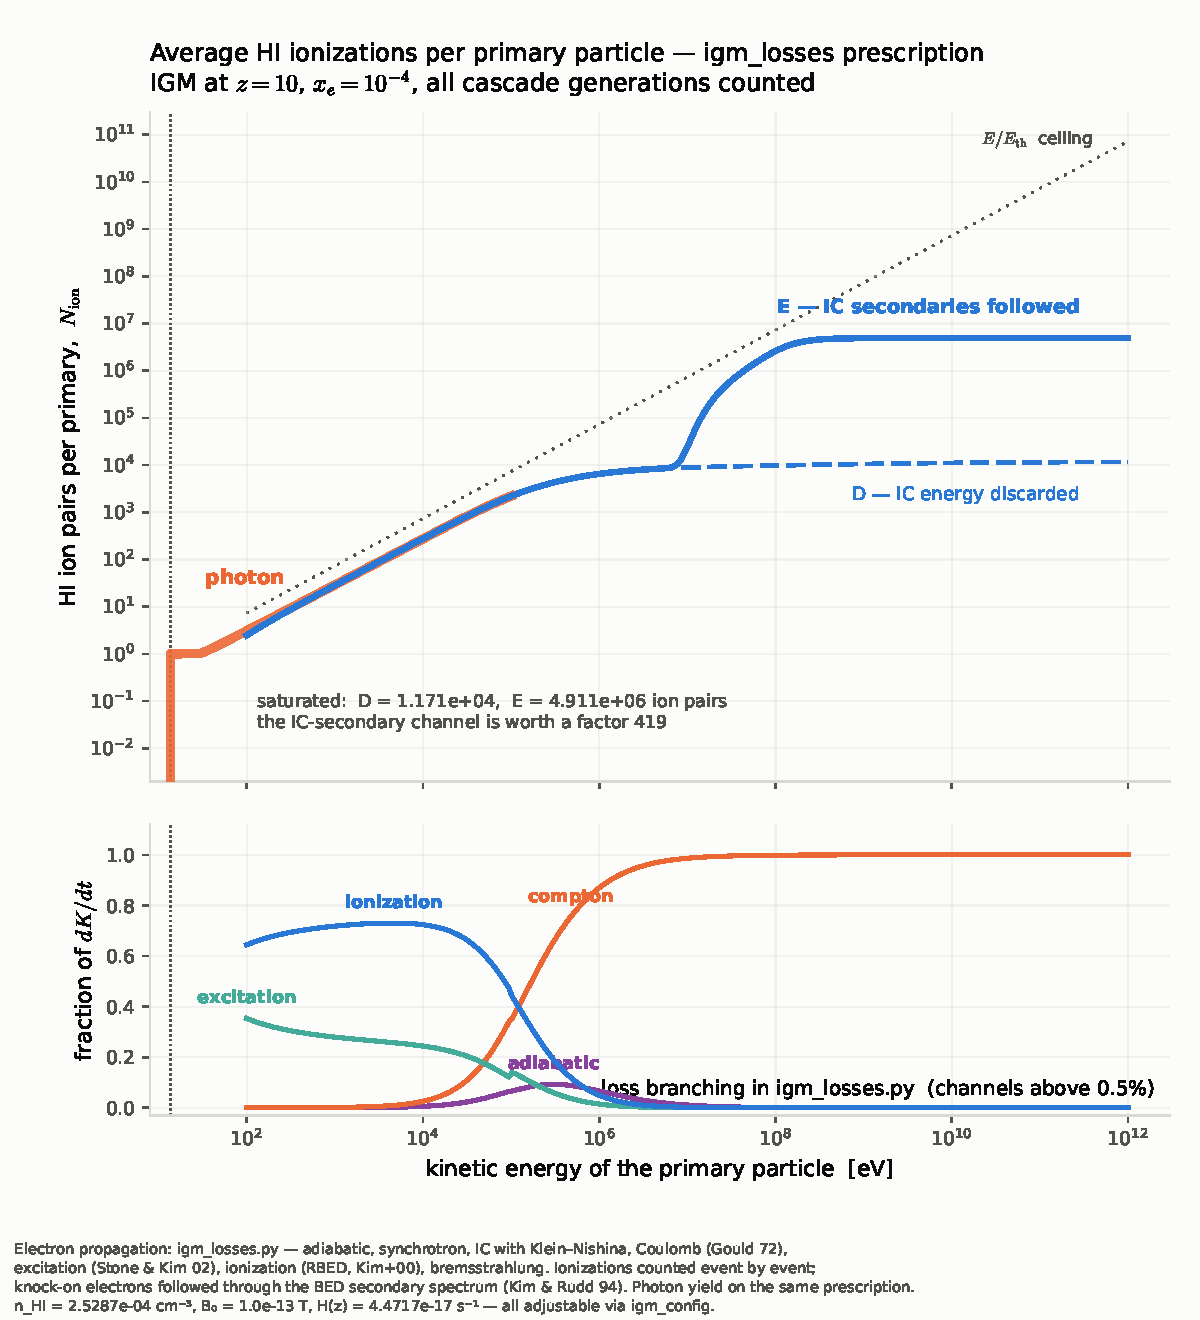
\includegraphics[width=0.72\textwidth]{ionization_yield_fig_igm.pdf}
\caption{\ion{H}{i} ion pairs per primary on the \texttt{igm\_losses}
prescription. \emph{Upper:} the loss routes and E with the photon curve on the same
prescription. \emph{Lower:} the seven-channel loss branching that sets the
shape --- adiabatic expansion reaches
$0.0929$\src{peakfrac\_adiabatic} of $dK/dt$, a channel the superseded
deposition-fit route did not have at all, while Coulomb
($0.002336$\src{peakfrac\_coulomb}), bremsstrahlung and synchrotron stay
negligible. Produced by \texttt{ionization\_yield\_igm.py}.}
\label{fig:yield}
\end{figure}
\paragraph{Reading Fig.~\ref{fig:yield}.} The upper panel plots the mean number
of \ion{H}{i} ion pairs a single primary produces, against its kinetic energy,
on logarithmic axes spanning fourteen decades in yield; the dotted diagonal is
the absolute ceiling $E/E_{\rm th}$, and the vertical dotted line marks the
$13.6$~eV threshold. Three curves are drawn: the photon yield (thick, orange),
and the two electron models --- \textbf{D} (dashed) which discards the energy
inverse Compton gives the CMB, and \textbf{E} (solid) which follows the
upscattered photons back down. \emph{Conclusion of the upper panel:} both
electron curves rise linearly while collisions dominate and then \emph{saturate},
D at $1.171\times10^{4}$\src{N\_e\_loss\_sat} ion pairs and E at
$4.911\times10^{6}$\src{N\_e\_loss\_ic\_sat}; the gap between them, a factor
$419.5$\src{lossic\_over\_loss\_sat}, \emph{is} the IC-secondary channel, and it is the
single largest effect in this figure. Neither curve crosses the ceiling.

The lower panel resolves where the primary's energy actually goes, plotting each
of the seven loss channels as a fraction of $dK/dt$. \emph{Conclusions of the
lower panel, in order of importance:} (i) \textbf{Compton overtakes the
collisional channels above $E_{\rm crit} =
1.487\times10^{5}$\src{E\_crit\_D\_eV}~eV, and that crossover is what saturates
the collisional yield} --- the two panels are the same statement told twice.
(ii) \textbf{Excitation is the largest irrecoverable sink.} It takes
$0.3532$\src{exc\_frac\_at\_100eV} of $dK/dt$ at the $100$~eV edge of the
plotted range --- still rising as $E$ falls, so this is an edge value and not a
turnover --- which is $151$\src{exc\_over\_next\_nonionizing} times the largest
other non-ionizing channel there. That energy leaves as Lyman-series photons,
every one of them below $13.6$~eV, so unlike the Compton share it can
\emph{never} come back as an ionization. (iii) \textbf{Adiabatic expansion
removes a real but modest amount of energy}: integrated over the whole cascade
it accounts for at most $7.696$\src{Efrac\_adiabatic\_max\_pct}\% of the
primary's energy, reached near $1$~MeV, and is negligible at both ends ---
$0.0145$\src{Efrac\_adiabatic\_1keV\_pct}\% at $1$~keV and
$0.000106$\src{Efrac\_adiabatic\_1TeV\_pct}\% at $1$~TeV, where Compton claims
$99.99$\src{Efrac\_compton\_1TeV\_pct}\% before anything else can act. Note that
this integrated figure is \emph{smaller} than the
$0.0929$\src{peakfrac\_adiabatic} peak visible in the panel, which is an
instantaneous rate share attained only near
$3.046\times10^{5}$\src{peakE\_adiabatic\_eV}~eV.
(iv) \textbf{Three channels are negligible everywhere}: Coulomb peaks at
$0.2336$\src{peak\_coulomb\_pct}\%, bremsstrahlung at
$0.00416$\src{peak\_bremsstrahlung\_pct}\% and synchrotron at
$1.18\times10^{-5}$\src{peak\_synchrotron\_pct}\%. Their smallness is the
quantitative licence for the superseded route to omit all three.


\subsection{Validation: two independent routes}
The superseded route (deposition fraction $f_{\rm ion}$, Bethe stopping,
Thomson-limit IC) shares nothing with the loss-based route but the physical
scenario. Below 1~MeV the two agree to between
$1.017$\src{loss\_over\_ic\_min} and $1.102$\src{loss\_over\_ic\_max}; at $10^{12}$~eV
the ratio is $1.32$\src{loss\_over\_ic\_1e12}, and that excess is Klein--Nishina ---
the old route used the Thomson limit, where the KN factor is
$0.8111$\src{F\_KN\_at\_1e12}. With the secondary channel carried on both sides
the agreement is $1.071$\src{lossic\_over\_depfit\_1e12}.

\subsection{Harmonisation of the two environments}\label{sec:harmonisation}
The two routes were built independently and therefore started from slightly
different fiducials. On 2026-09-11 you chose to keep the route-1 values in both,
and \texttt{igm\_losses.py} was edited accordingly: the ionization threshold
became the NIST value $13.598435$~eV rather than one Rydberg, and
$n_{\rm HI}$ was renormalised from Planck 2018 plus PDG 2022. Two of the three
environmental inputs now agree exactly; the third does not, and is reported
rather than hidden:
\begin{center}\small
\begin{tabular}{llll}
\hline
quantity & route 1 & route 2 & fractional difference \\
\hline
$n_{\rm H}$ & \multicolumn{2}{c}{identical by construction} &
  $1.05\times10^{-10}$\src{env\_dn\_H} (round-off) \\
$E_{\rm th}$ & \multicolumn{2}{c}{$13.598435$~eV, NIST} &
  $0$\src{env\_dE\_th} \\
$H(z)$ & hard-coded Planck 18 & \texttt{astropy} Planck 18 &
  $0.001369$\src{env\_dH\_z} \\
\hline
\end{tabular}
\end{center}
The residual in $H(z)$ is two different evaluations of the \emph{same}
cosmology, not two cosmologies. It reaches the yield only through the adiabatic
loss term, whose own peak share of $dK/dt$ is
$0.0929$\src{peakfrac\_adiabatic}, so its effect on any number in this document
is below $10^{-4}$ in relative terms. \textbf{It has not been harmonised, and
that is a pending decision, not an oversight.}

\begin{figure}[h]\centering
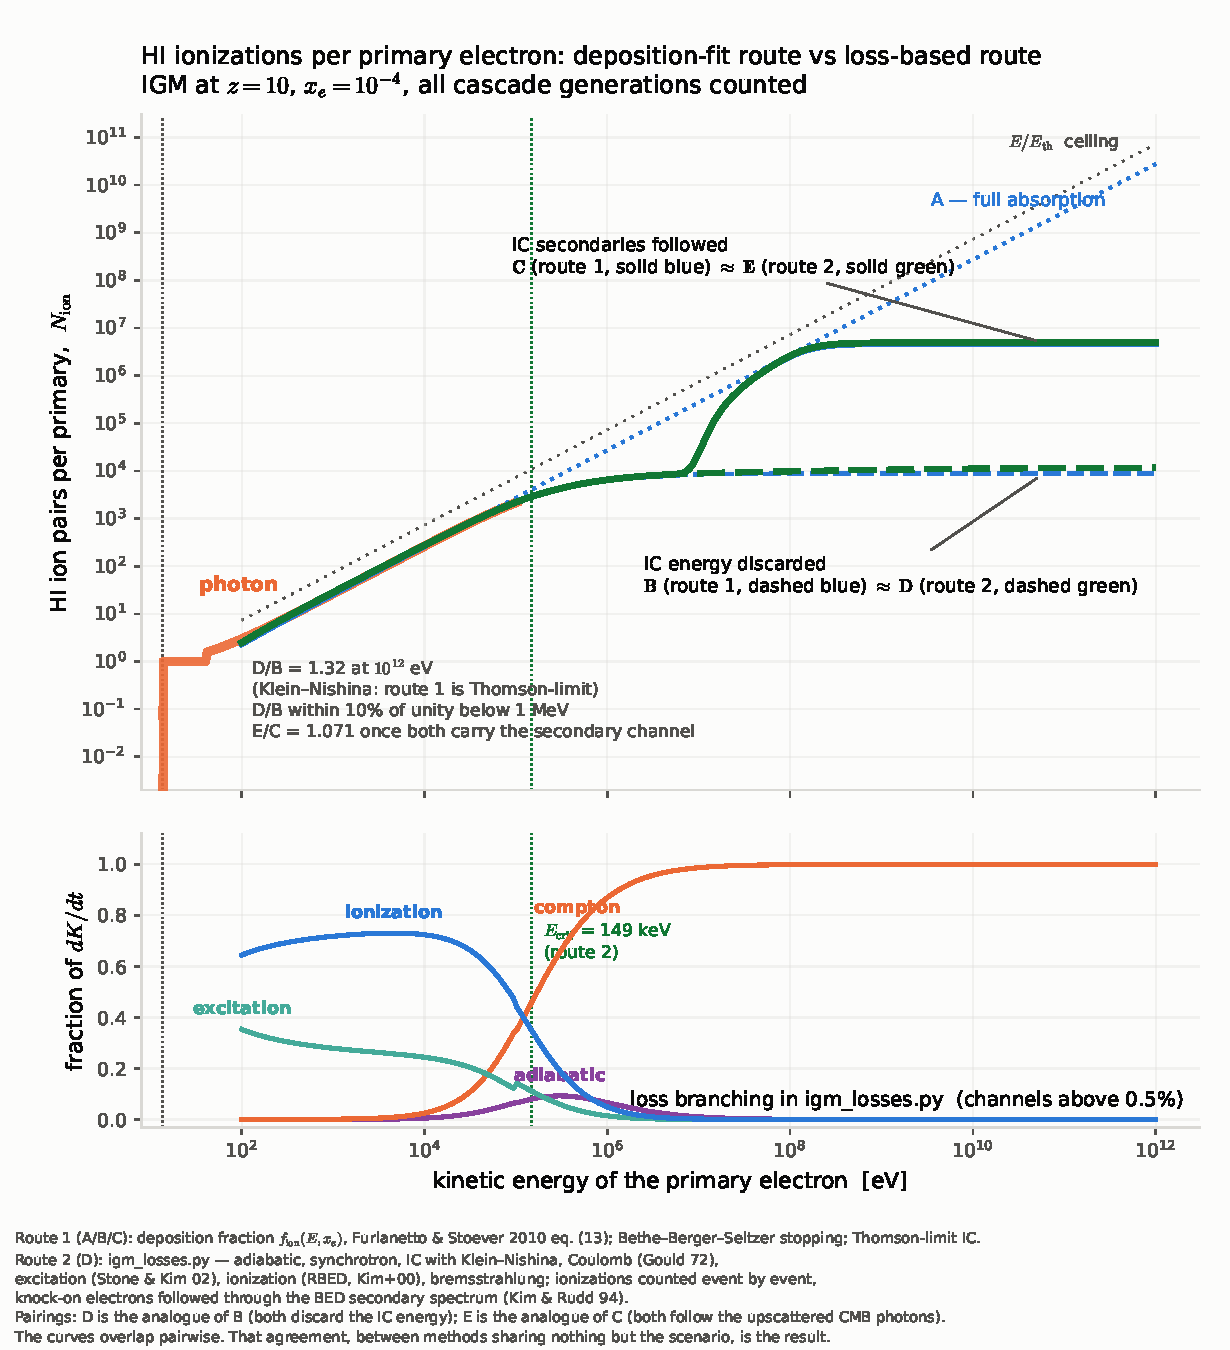
\includegraphics[width=0.92\textwidth]{yield_comparison_fig.pdf}
\caption{The two routes on the same axes; the curves overlap pairwise (D with
B, E with C), which is the result. \emph{Lower panel:} the loss branching.
The two environments are now \emph{harmonised} on the route-1 values
(\S\ref{sec:harmonisation}): the fractional difference in $n_{\rm H}$ is
$1.05\times10^{-10}$\src{env\_dn\_H}, i.e.\ floating-point round-off, and the
ionization threshold agrees exactly,
$\Delta E_{\rm th}=0$\src{env\_dE\_th}~eV. Any residual disagreement between
the routes is therefore physics, not input. Produced by \texttt{yield\_comparison.py}.}
\label{fig:validation}
\end{figure}
\paragraph{Reading Fig.~\ref{fig:validation}.} This figure exists to be
\emph{boring}. It overlays the two independent routes on one set of axes: the
deposition-fit route (models A, B, C; blue) and the loss-based route (the loss routes,
E; green), paired by what they assume about the inverse-Compton energy --- B
with D discard it, C with E follow it. \emph{Conclusion:} \textbf{the curves
overlap pairwise, and that agreement is the result.} Below 1~MeV the two routes
agree to between $1.017$\src{loss\_over\_ic\_min} and $1.102$\src{loss\_over\_ic\_max};
with the secondary channel carried on both sides the agreement at $10^{12}$~eV
is $1.071$\src{lossic\_over\_depfit\_1e12}. The one visible divergence, $D/B =
1.320$\src{loss\_over\_ic\_1e12} at $10^{12}$~eV, is \emph{not} a disagreement about
physics but about Klein--Nishina: the superseded route used the Thomson limit,
where the KN factor has already fallen to
$0.8111$\src{F\_KN\_at\_1e12}. Since the two routes share nothing but the
physical scenario --- one is a published deposition fit, the other counts
ionization events against RBED cross sections --- this is the strongest single
piece of evidence in the document. The lower panel repeats the loss branching of
Fig.~\ref{fig:yield} with $E_{\rm crit}$ marked, and supports the same four
conclusions listed there.


\clearpage
\section{Result}\label{sec:result}
\begin{figure}[h]\centering
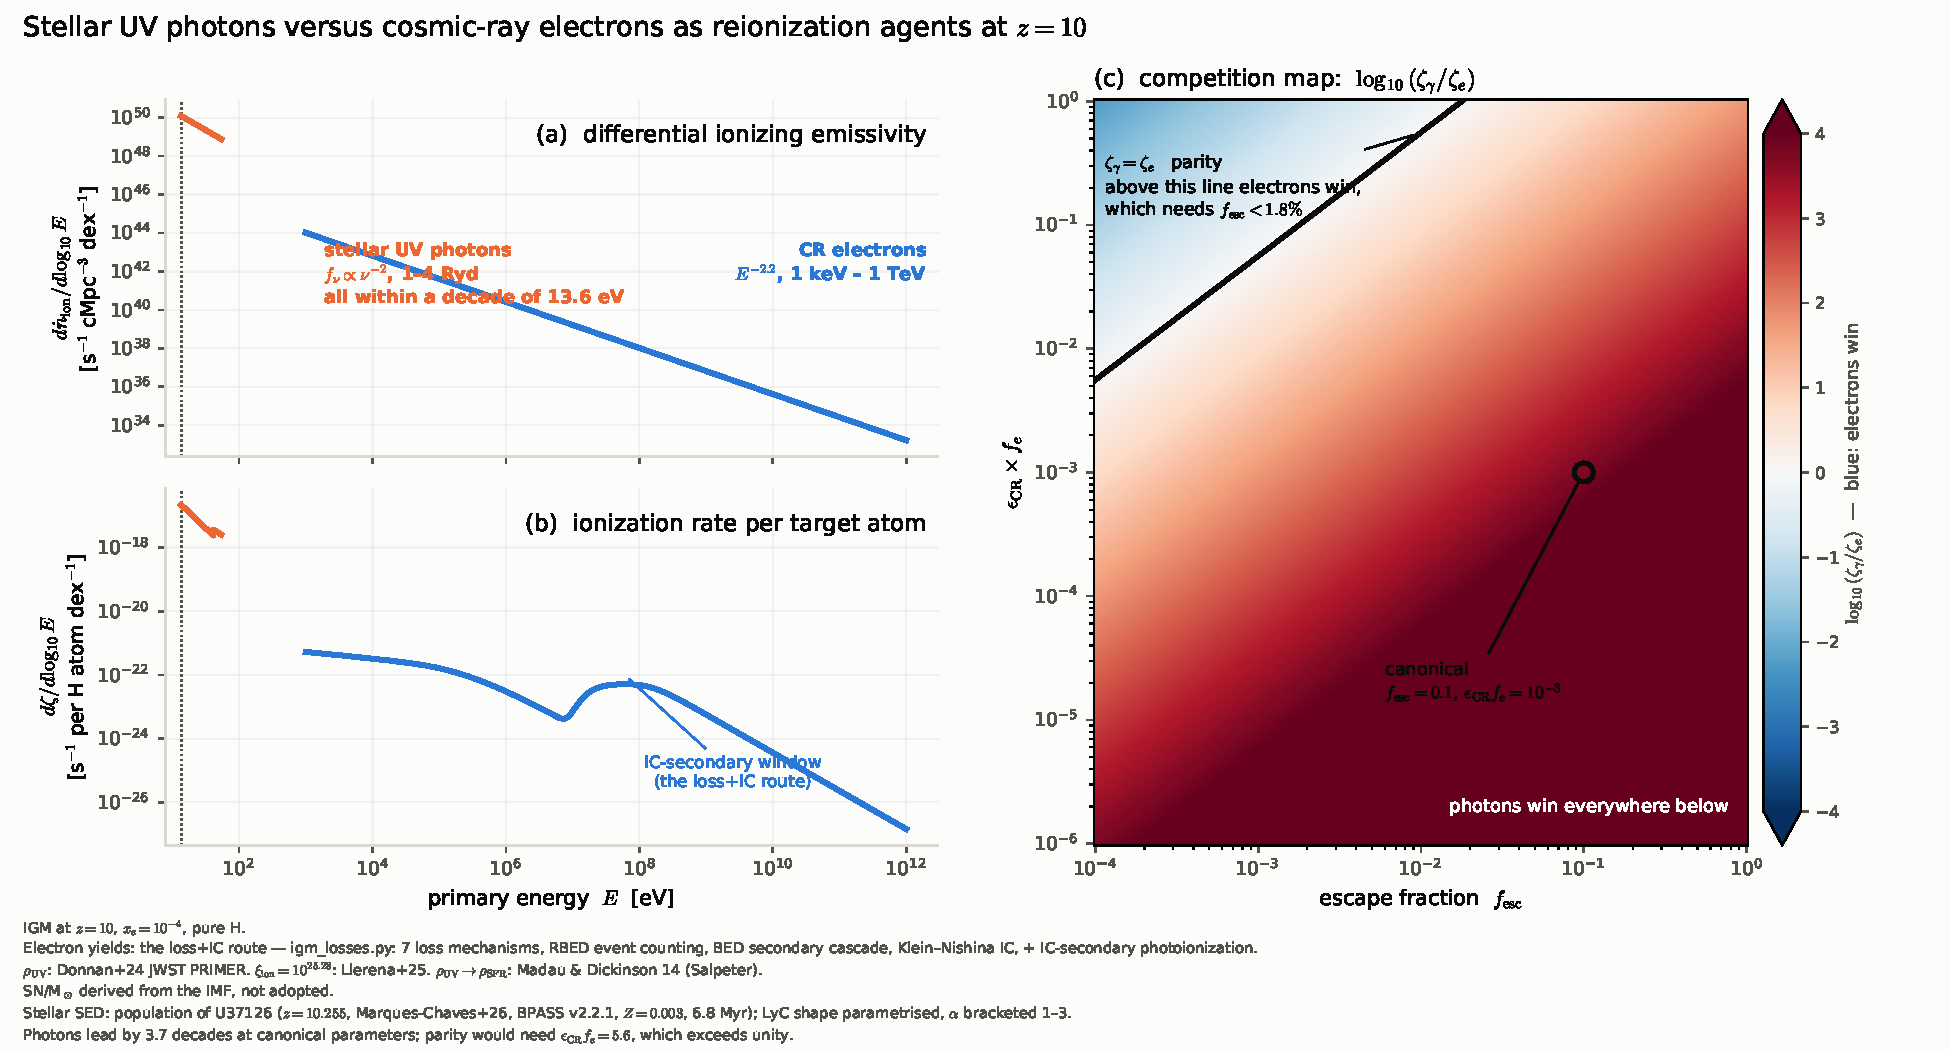
\includegraphics[width=\textwidth]{photon_vs_electron_fig1.pdf}
\caption{(a) differential ionizing emissivity and (b) ionization rate per target
atom, for both channels, with (c) the competition map over the two scanned
normalisations. Colour encodes channel throughout. The bump near $10^{8}$~eV in
(b) is the IC-secondary window of the yield model. Produced by
\texttt{photon\_vs\_electron.py::make\_figures}.}
\label{fig:result}
\end{figure}
\paragraph{Reading Fig.~\ref{fig:result}.} Panel (a) is the differential
ionizing emissivity $d\dot n_{\rm ion}/d\log_{10}E$ of each channel, panel (b)
the same quantity divided by the target density to give the ionization rate per
hydrogen atom $d\zeta/d\log_{10}E$, and panel (c) the competition map
$\log_{10}(\zeta_\gamma/\zeta_e)$ over the two scanned normalisations.

\emph{Conclusion of panel (a) --- and it is a warning about how to read the
figure at all:} \textbf{the two channels do not live at the same energies.} The
escaping stellar band is confined to
$0.6023$\src{photon\_band\_dex}~dex, from $13.598$ to
$54.42$\src{photon\_band\_hi\_eV}~eV (1--4~Ryd by construction), while the CR
electrons span $9.00$\src{electron\_band\_dex}~dex --- a range
$14.94$\src{band\_dex\_ratio} times wider --- and the two do not even touch:
$1.264$\src{band\_gap\_dex}~dex of empty axis separates the top of the photon
band from the bottom of the electron band. \textbf{Nothing can therefore be
concluded by comparing the heights of the two curves in this panel}; the
comparison only becomes meaningful once integrated over energy, which is exactly
what $\zeta$ is.

\emph{Conclusion of panel (b):} the same statement in per-atom units, plus one
feature of the yield model made visible --- the bump is the IC-secondary
window, $2.022\times10^{7}$\src{Ewindow\_lo\_eV} to
$3.554\times10^{8}$\src{Ewindow\_hi\_eV}~eV, the energies at which an electron
upscatters CMB photons past $13.6$~eV but below the escape energy
$1218.0$\src{audit\_E\_esc\_z10\_eV}~eV. \emph{Conclusion of panel (c):}
\textbf{photons win over essentially the whole physically allowed plane.} The
parity locus requires $f_{\rm esc} <
1.786$\src{fesc\_parity\_pct\_z10}\%, and at canonical parameters the ratio is
$5599$\src{zeta\_ratio}, i.e.\ $3.748$\src{zeta\_ratio\_decades} decades.


\begin{itemize}\itemsep2pt
\item $\zeta_\gamma = 4.647\times10^{-18}$\src{zeta\_gamma\_s}
      $\mathrm{s^{-1}}$ per \ion{H}{i} atom, with the propagated interval
      $[1.470\times10^{-18}\src{zeta\_gamma\_lo},\,
        1.436\times10^{-17}\src{zeta\_gamma\_hi}]\ \mathrm{s^{-1}}$.
      The interval adds the $\rho_{\rm UV}$ and $\xi_{\rm ion}$ errors
      \emph{linearly in dex}, which is conservative rather than a quadrature;
      see \S\ref{sec:audit} item~1 for the correction to its lower end.
\item $\zeta_e = 8.299\times10^{-22}\src{zeta\_e\_s}\ \mathrm{s^{-1}}$ per atom.
      \textbf{No error bar is quoted, and that is a limitation:}
      $\epsilon_{\rm CR}$ and $f_e$ are unmeasured at $z=10$, which is exactly
      why they are scanned rather than fitted.
\item Ratio $5599$\src{zeta\_ratio}, i.e.\
      $3.748$\src{zeta\_ratio\_decades} decades in favour of stellar UV.
\item Parity needs $\epsilon_{\rm CR}f_e = 5.6$\src{eps\_cr\_fe\_crossover},
      which exceeds unity and is therefore unreachable.
\end{itemize}



\subsection{Two normalisations: \texorpdfstring{$t_H$}{t_H} and
            \texorpdfstring{$t_{\rm rec}$}{t_rec}}\label{sec:norm}
$\zeta$ is a rate per atom, $\mathrm{s^{-1}}$. To say anything with it you
multiply by a clock, and \emph{the choice of clock changes the question being
asked}. Both clocks are used in the literature and they are not
interchangeable.

\paragraph{The Hubble time, $t_H = 1/H(z)$ --- a \emph{budget} question.}
$\zeta t_H$ is the number of times the channel ionizes each atom while the
universe expands by an $e$-fold. It asks ``are there enough photons at all?''
Reaching $\zeta t_H \simeq 1$ is necessary merely to touch every atom once, and
it ignores that an atom ionized early can recombine and need ionizing again.

\paragraph{The recombination time --- a \emph{maintenance} question, and the
standard one.} This is the normalisation you were right to expect. Madau \&
Dickinson~\cite{md14}, eq.~(24), give the volume-averaged
\ion{H}{i} recombination timescale
\begin{equation}
  \langle t_{\rm rec}\rangle = \bigl(\chi\,\langle n_{\rm H}\rangle\,
  \alpha_B\,C_{\rm IGM}\bigr)^{-1}
  \simeq 3.2\ \mathrm{Gyr}\ \Bigl(\tfrac{1+z}{7}\Bigr)^{-3} C_{\rm IGM}^{-1},
  \label{eq:trec}
\end{equation}
with $\chi = 1.08$ for the photoelectrons from singly ionized helium,
$\alpha_B$ the case-B coefficient at $T = 2\times10^4$~K, and $C_{\rm IGM} = 1 +
43\,z^{-1.71}$. \paragraph{Eq.~\eqref{eq:trec} factor by factor.} Every factor is named, valued
and sourced below. Two of them are \emph{derived} here rather than adopted, and
one is traced back past \cite{md14} to the paper it actually comes from ---
because the shorthand ``$1 + 43\,z^{-1.71}$'' is not what that paper prints.
Checks \texttt{B3}, \texttt{B7}--\texttt{B11} of
\texttt{reionization\_budget.py}.

\begin{center}\footnotesize
\renewcommand{\arraystretch}{1.35}
\begin{tabular}{|c|p{4.6cm}|p{3.0cm}|p{4.5cm}|}
\hline
factor & what it is & value here & where it comes from \\
\hline
$(\;\cdots)^{-1}$
  & The bracket $\chi\langle n_{\rm H}\rangle\alpha_B C_{\rm IGM}$ is the
    recombination rate \emph{per ionized hydrogen atom}, $R/n_{\rm HII}$ at
    $x=1$; its reciprocal is the mean time for one ion to recombine once.
  & ---
  & Definition. Follows from eq.~\eqref{eq:zetacrit}. \\
\hline
$\chi$
  & Electrons per ionized hydrogen. Helium donates one electron per atom once
    singly ionized, so $n_e = n_{\rm HII}+n_{\rm HeII} = n_{\rm H}(1+n_{\rm He}/n_{\rm H})$.
  & $1.0811$\src{chi\_derived}
  & \cite{md14} eq.~(24) quote $1.08$. \textbf{Derived here} from
    $Y_P = 0.245$\src{Y\_P}: $\chi = 1+(Y_P/4)/X_H$. \\
\hline
$\langle n_{\rm H}\rangle$
  & \emph{Volume-averaged} hydrogen number density. The average matters:
    recombination goes as $n^2$, and $\langle n^2\rangle\ne\langle n\rangle^2$.
    That discrepancy is exactly what $C_{\rm IGM}$ carries.
  & $2.5287\times10^{-4}$\src{n\_H\_cm3\_z10}~cm$^{-3}$ at $z=10$
  & This work's harmonised value (\S\ref{sec:harmonisation}): Planck 2018
    $\Omega_b h^2$ with the PDG 2022 $\rho_{\rm crit}$. \\
\hline
$\alpha_B$
  & Recombination coefficient, \textbf{case B}: recombinations to the $n=1$
    level are \emph{excluded}, because the photon they emit is reabsorbed on
    the spot and ionizes another atom, so it is no net recombination.
  & $1.430\times10^{-13}$\src{alpha\_B\_2e4K}~cm$^3$s$^{-1}$ at
    $T = 2\times10^4$~K
  & Osterbrock \& Ferland~\cite{of06} Table 2.1, at the $T$ \cite{md14} assume.
    \textbf{Confirmed independently} against the Hui \& Gnedin~\cite{hg97} fit:
    $1.4277\times10^{-13}$\src{alpha\_B\_HG97\_2e4}. \\
\hline
$C_{\rm IGM}$
  & Clumping factor $\langle n_{\rm H}^2\rangle/\langle n_{\rm H}\rangle^2$ of
    the \emph{ionized} hydrogen. It converts the mean-density recombination
    rate into the true volume-averaged one.
  & $1.8384$\src{C\_MD14\_z10} at $z=10$
  & Pawlik, Schaye \& van Scherpenzeel~\cite{pawlik09} --- see below. \\
\hline
$3.2$~Gyr
  & The bracket evaluated at $(1+z)/7 = 1$ with $C_{\rm IGM}=1$; a convenience
    normalisation, not an independent input.
  & $3.1487$\src{t\_rec\_z6\_C1\_Gyr}~Gyr recomputed
  & \cite{md14} eq.~(24). \textbf{Reproduced here} from our own
    $n_{{\rm H}0}$, to $1.6\%$. \\
\hline
$\bigl(\tfrac{1+z}{7}\bigr)^{-3}$
  & The $(1+z)^3$ dilution of a comoving density, referred to $z=6$. It is the
    whole redshift dependence of $t_{\rm rec}$ at fixed $C$.
  & ---
  & Definition; $\langle n_{\rm H}\rangle\propto(1+z)^3$. \\
\hline
\end{tabular}
\end{center}

\paragraph{Why $\chi$ is $1.08$ and not $1$ or $1.16$.} With
$Y_P = 0.245$\src{Y\_P} and $X_H = 0.755$\src{X\_H}, the helium-to-hydrogen
number ratio is $(Y_P/4)/X_H = 0.08113$\src{n\_He\_over\_n\_H}, so singly
ionized helium raises the electron density by that fraction and
$\chi = 1.0811$\src{chi\_derived} --- agreeing with \cite{md14}'s $1.08$ to
$0.1\%$. \textbf{Were helium doubly ionized}, $\chi$ would be
$1.1623$\src{chi\_HeIII}; that is the value appropriate \emph{after} HeII
reionization at $z\lesssim3$ and emphatically not at $z\ge5.5$. So $\chi$ is
not a fudge factor --- it is the electron-per-proton ratio of a specific
ionization state, and using the wrong state would be a $7\%$ error.

\paragraph{Where ``$1 + 43\,z^{-1.71}$'' really comes from.}
\cite{pawlik09} do not print that expression. Their eq.~(A1) is
\begin{equation}
  C(z) = z^{\beta}\,e^{-\gamma z + \delta} + \alpha ,
  \label{eq:pawlik}
\end{equation}
and their Table~A1 gives, for $C_{100}$ in the \texttt{r19.5L6N256} run,
$\alpha = 1.00$, $\beta = -1.71$, $\gamma = 0.00$, $\delta = 3.76$. Substituting,
$C_{100}(z) = 1 + e^{3.76}z^{-1.71}$, and
$e^{3.76} = 42.95$\src{pawlik\_exp\_delta} --- \textbf{that is \cite{md14}'s
``43''}. Evaluating eq.~\eqref{eq:pawlik} directly against the shorthand agrees
to $0.084$\src{C\_pawlik\_vs\_MD14\_maxreldiff\_pct}\% at $z = 20$, $10$ and
$5.5$. Two things follow that the shorthand hides:
\begin{itemize}\itemsep2pt
\item \textbf{It is $C_{100}$}: the clumping of gas \emph{below} overdensity
      $100$, from the simulation reheated at $z_r = 19.5$. Gas above that
      threshold sits in collapsed, self-shielding structures and is excluded on
      purpose. \cite{pawlik09}'s $C_{-1}$, which counts all gas, is about twice
      as large at $z=6$ --- so this choice is the \emph{less} demanding one, and
      the $C = 3$ and $C = 12$ columns of Tables~\ref{tab:budget}
      and~\ref{tab:budgettrec} are there to bracket it.
\item \textbf{Its fitted range is $6$\src{pawlik\_fit\_z\_lo} $\le z \le$ $20$\src{pawlik\_fit\_z\_hi}}.
      $z=20$ sits exactly at the upper edge and $z=10$ well inside, but
      \textbf{$z = 5.5$ is below it}: the $C_{\rm IGM}$ entry at $z=5.5$ is an
      extrapolation --- mild, $0.5$ in $z$, but real, and it is the only cell in
      either table that leaves a source's stated domain. The fixed-$C$ columns
      assume nothing and are unaffected.
\end{itemize}

\paragraph{The temperature is the one silent assumption.}
$\alpha_B$ is the only factor with a free knob, and $T$ is an assumption about
photoionized gas rather than a measurement of this IGM. Since
$t_{\rm rec}\propto\alpha_B^{-1}$ and $\alpha_B$ \emph{falls} with $T$, a hotter
assumed IGM lengthens $t_{\rm rec}$ and \emph{lowers} the requirement. Between
the two values in common use the recombination term changes by
$1.815$\src{alpha\_B\_ratio\_1e4\_over\_2e4}: at $z=10$ with the
\cite{md14} clumping, $N_{\rm req}$ moves from
$2.606$\src{Nreq\_z10\_CMD14} at their $2\times10^4$~K to
$3.915$\src{Nreq\_z10\_CMD14\_at\_1e4K} at $10^4$~K. \textbf{So \cite{md14}'s
temperature choice is the milder of the two}, and $T$ is the second-largest
lever in the budget after $C$. Both are stated here rather than buried in
$\alpha_B$.

The criterion is then simply
\[
  \zeta\,t_{\rm rec} \ge 1
  \quad\Longleftrightarrow\quad
  \text{ionizations outpace recombinations,}
\]
i.e.\ the gas can be \emph{kept} ionized. Recomputing eq.~\eqref{eq:trec} from
this work's own $n_{\rm H}$ rather than quoting it returns
$3.149$\src{t\_rec\_z6\_C1\_Gyr}~Gyr at $(1+z)/7 = 1$ and $C_{\rm IGM}=1$
against their $3.2$~Gyr, and $t_{\rm rec}/t_H =
0.6228$\src{t\_rec\_over\_t\_H} at $z=10$ against their ``$\sim$60\% of the
expansion timescale'' --- so the machinery agrees with the source it cites.

\paragraph{What the two say here.} With $C_{\rm IGM} =
1.838$\src{C\_IGM} at $z=10$,
\begin{center}\small
\begin{tabular}{lll}
\hline
 & $z=10$ & $z=20$ \\
\hline
$t_{\rm rec}/t_H$                & $0.6228$\src{t\_rec\_over\_t\_H}
                                 & $0.3457$\src{t\_rec\_over\_t\_H\_z20} \\
$\zeta_\gamma t_H$               & $0.1039$\src{zeta\_gamma\_tH}
                                 & $0.03937$\src{zeta\_gamma\_tH\_z20} \\
$\zeta_\gamma t_{\rm rec}$       & $0.06472$\src{zeta\_gamma\_trec}
                                 & $0.01361$\src{zeta\_gamma\_trec\_z20} \\
$\zeta_e t_{\rm rec}$            & $1.156\times10^{-5}$\src{zeta\_e\_trec}
                                 & $2.368\times10^{-6}$\src{zeta\_e\_trec\_z20} \\
required, $1+t_H/t_{\rm rec}$    & $2.606$\src{ion\_per\_atom\_needed\_per\_tH}
                                 & $3.892$\src{ion\_per\_atom\_needed\_per\_tH\_z20} \\
\hline
\end{tabular}
\end{center}
\emph{The $z=20$ column of the two $\zeta$ rows carries the unanchored
$\rho_{\rm UV}$ of \S\ref{sec:z20}} --- no measurement exists at that redshift,
so those two entries inherit the $z=10$ normalisation and should be read with
the factor-$10^3$ ignorance band attached. The three rows that contain no
$\rho_{\rm UV}$ --- $t_{\rm rec}/t_H$, $C_{\rm IGM}$ and the requirement --- are
exact at both redshifts.
The two normalisations differ by exactly $t_{\rm rec}/t_H$, nothing more. At
$z=10$ that factor is $0.62$, so they happen to give numbers within a factor
$1.6$ of each other and the same verdict --- \textbf{but that near-coincidence
is specific to this redshift.} At fixed clumping $t_{\rm rec}\propto(1+z)^{-3}$
while $t_H\propto(1+z)^{-3/2}$ in matter domination, so $t_{\rm rec}/t_H$ would
scale as $(1+z)^{-3/2}$, a factor $0.379$ between the two redshifts. The
measured factor is $0.555$, and the difference is $C_{\rm IGM}$: it
falls from $1.838$\src{C\_IGM} to $1.256$\src{C\_IGM\_z20}, lengthening
$t_{\rm rec}$ by $1.463$ and partly offsetting the density rise
($0.379\times1.463 = 0.5548$ against the measured $0.5551$, a $0.06\%$
residual which is $\Lambda$ and radiation in the exact $H(z)$ --- so the
decomposition is checked, not asserted). Either way the direction is the same:
by $z=20$ the ratio has fallen to $0.3457$\src{t\_rec\_over\_t\_H\_z20} and the
maintenance criterion is \emph{harder}, not easier. Reading a $\zeta t_H$ as
though it were a $\zeta t_{\rm rec}$ therefore gets steadily more wrong with
redshift.

\paragraph{Regarding the total value: neither clock alone is the requirement.}
Over any interval the ionizations per atom must satisfy $N \ge 1 + N_{\rm rec}$
--- one to ionize the atom, plus one per recombination it suffers. Per Hubble
time that is $1 + t_H/t_{\rm rec} =
2.606$\src{ion\_per\_atom\_needed\_per\_tH} at $z=10$, which is precisely
\cite{md14}'s ``close to two ionizing photon per baryon \dots\ needed to keep
the IGM ionized''. Against that requirement:
\begin{itemize}\itemsep2pt
\item the stellar channel supplies $0.1039$\src{zeta\_gamma\_tH}, short by a
      factor $25.1$\src{reion\_shortfall\_factor};
\item the cosmic-ray channel is short by
      $1.404\times10^{5}$\src{reion\_shortfall\_factor\_CR}.
\end{itemize}

\paragraph{What the shortfall does and does not mean.} It is \emph{not} a
failure of this calculation, and it is not evidence against stellar
reionization. It is the statement that $z=10$ lies \emph{inside} reionization
rather than at its end: the escaping stellar output at $z=10$ cannot yet hold
the IGM ionized, which is exactly what a substantially neutral $z=10$ IGM
means. Completing reionization near $z\approx6$ is done by the steep rise of
$\rho_{\rm SFR}$ between $z=10$ and $z\approx6$, and \textbf{this document
adopts no star-formation history}, so that closing is reported as missing
rather than asserted. What the shortfall \emph{does} do is sharpen this paper's
conclusion: if the channel that actually reionizes the universe is already a
factor $25$ short at $z=10$, the cosmic-ray channel --- a further
$5599$\src{zeta\_ratio} below it --- is not a candidate under any bookkeeping.

\paragraph{Correction.} Earlier versions of this document reported
$\zeta_\gamma t_H = 0.1037$ and called it ``the pace required for reionization
to complete near $z\approx6$''. That was wrong twice: the standard clock for
this comparison is $t_{\rm rec}$, not $t_H$, and the value is a factor
$25.1$\src{reion\_shortfall\_factor} \emph{below} the requirement rather than
at it. The check that asserted it, C32, tested only $0.01 < \zeta_\gamma t_H <
3$ --- a window wide enough to accept almost anything --- and has been replaced
by three checks that compare against eq.~\eqref{eq:trec} and state the
shortfall.

\subsection{Parameter exploration}
Both layouts are kept, as requested, so the same content can be read either as
one panel set or as two separate figures.

\begin{figure}[h]\centering
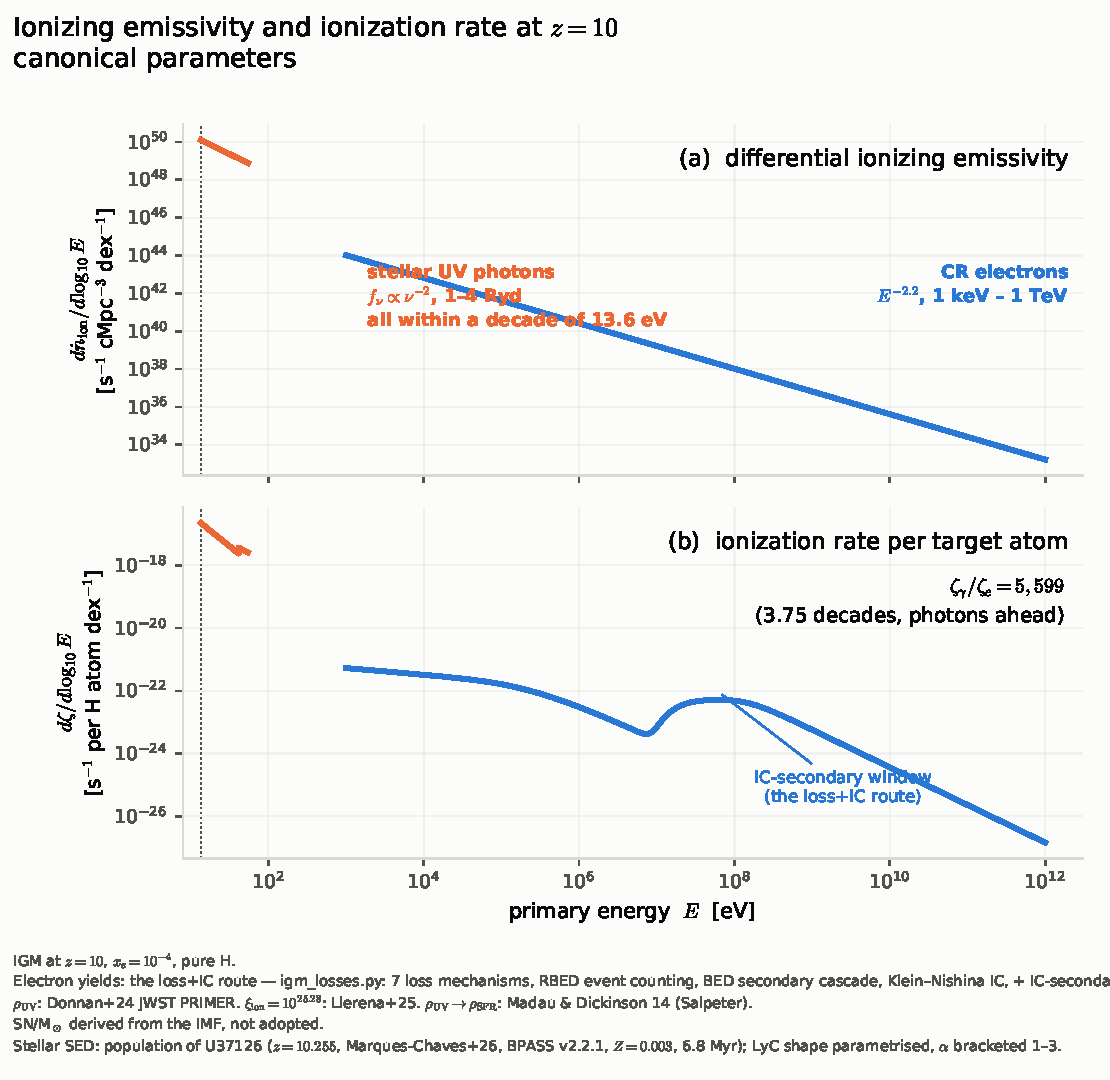
\includegraphics[width=0.70\textwidth]{photon_vs_electron_fig2a.pdf}
\caption{Panels (a) and (b) alone, at canonical parameters. Produced by
\texttt{photon\_vs\_electron.py::make\_figures}.}
\label{fig:2a}
\end{figure}
\paragraph{Reading Fig.~\ref{fig:2a}.} Panels (a) and (b) of
Fig.~\ref{fig:result} again, at canonical parameters and without the map, for
readers who want the two spectra larger. The content and both conclusions are
those given for Fig.~\ref{fig:result}: the channels occupy disjoint energy
ranges separated by $1.264$\src{band\_gap\_dex}~dex, so only the integrated
$\zeta$ is comparable, and the IC-secondary window
($2.022\times10^{7}$\src{Ewindow\_lo\_eV}--$3.554\times10^{8}$\src{Ewindow\_hi\_eV}~eV)
shows as the bump in panel (b). Kept because both layouts were requested; it carries
no conclusion of its own.


\begin{figure}[h]\centering
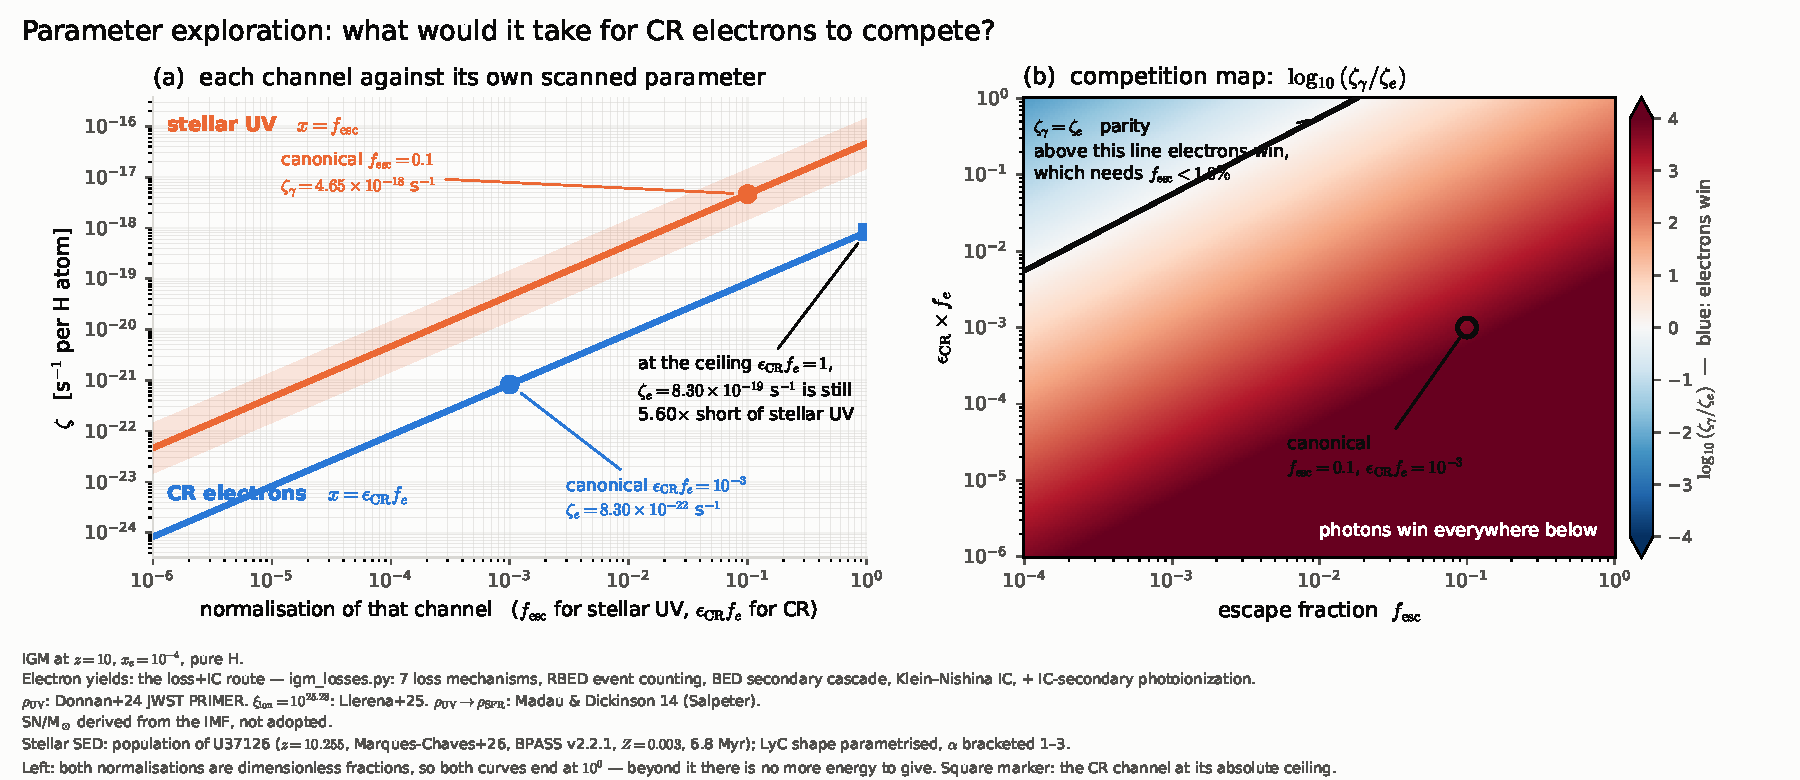
\includegraphics[width=0.98\textwidth]{photon_vs_electron_fig2b.pdf}
\caption{Each channel against its own normalisation, and the competition map.
Both normalisations are dimensionless fractions, so both curves end at $10^0$:
at the ceiling $\epsilon_{\rm CR}f_e = 1$ --- every erg of every supernova into
electrons --- the CR channel is still short of stellar UV by the factor
$5.599$\src{eps\_cr\_fe\_crossover}. \emph{Note:} the map's colour scale is
clipped at $\pm4$ while the data span $-2.25$ to $+7.75$ decades; the parity
contour and the canonical marker are exact, the saturated corners are not.
Produced by \texttt{photon\_vs\_electron.py::make\_figures}.}
\label{fig:2b}
\end{figure}
\paragraph{Reading Fig.~\ref{fig:2b}.} The left panel plots each channel's
$\zeta$ against \emph{its own} scanned normalisation --- $f_{\rm esc}$ for
stellar UV, $\epsilon_{\rm CR}f_e$ for cosmic rays --- with the shaded band the
published $\pm1\sigma$ on $\rho_{\rm UV}$, filled circles at the canonical
values and a square at the CR channel's absolute ceiling. The right panel is the
competition map of Fig.~\ref{fig:result}(c).

\emph{Conclusion of the left panel:} \textbf{both curves end at $10^{0}$ and
cannot be extended.} Both normalisations are dimensionless fractions bounded by
unity --- beyond $f_{\rm esc} = 1$ there are no photons left to escape, and
beyond $\epsilon_{\rm CR}f_e = 1$ there is more energy in cosmic-ray electrons
than the supernova released. At that ceiling the CR channel is \emph{still}
short of stellar UV by a factor
$5.599$\src{eps\_cr\_fe\_crossover}, which is the whole argument of this
document in one number: \textbf{parity is not merely unlikely, it is outside the
physically available range}. \emph{Conclusion of the right panel:} as for
Fig.~\ref{fig:result}(c). Note the caveat already stated in the caption --- the
colour scale is clipped at $\pm4$ while the data span $-2.25$ to $+7.75$
decades, so the saturated corners are not quantitative, though the parity locus
and the canonical marker are exact.

\clearpage
% ===========================================================================
\section{The same calculation at \texorpdfstring{$z=20$}{z = 20}}\label{sec:z20}
% ===========================================================================
Every figure in this folder was regenerated at an initial redshift $z=20$ with
the same code, driven by \texttt{run\_redshift\_suite.py}. Nothing in the
physics was re-derived by hand; what changed are the environmental inputs, and
this section states exactly which, because that is where a redshift change
silently goes wrong.

\subsection{What scales with \texorpdfstring{$z$}{z}, and where it enters}
\begin{center}\small
\begin{tabular}{llll}
\hline
quantity & scaling & $z=10$ & $z=20$ \\
\hline
$n_{\rm HI}$ [cm$^{-3}$] & $(1+z)^3$ &
  $2.528723\times10^{-4}$\src{n\_H\_cm3\_route1} &
  $1.759467\times10^{-3}$\src{n\_H\_cm3\_route1\_z20} \\
  & & \multicolumn{2}{l}{ratio
  $6.958$\src{n\_H\_ratio\_z20\_over\_z10}} \\
$H(z)$ [s$^{-1}$] & Planck 18 &
  $4.471729\times10^{-17}$\src{H\_z\_s\_route2} &
  $1.180246\times10^{-16}$\src{H\_z\_s\_route2\_z20} \\
  & & \multicolumn{2}{l}{ratio $2.639$\src{H\_ratio\_z20\_over\_z10}} \\
$T_{\rm CMB}$ & $(1+z)$ & \multicolumn{2}{l}{$U_{\rm CMB}\propto(1+z)^4$:
  a factor $13.28$\src{U\_CMB\_ratio\_z20\_over\_z10} between the two} \\
$B$ & $B_0(1+z)^2$ & \multicolumn{2}{l}{synchrotron stays below $10^{-5}$ of
  $dK/dt$ at both redshifts} \\
\hline
\end{tabular}
\end{center}
All four reach the calculation through \texttt{igm\_losses.py}; the target
density and $H(z)$ additionally reach the route-1 cross-check through
\texttt{ionization\_yield.cosmology}. The harmonisation of
\S\ref{sec:harmonisation} carries over unchanged: at $z=20$ the $n_{\rm H}$
residual is again $1.05\times10^{-10}$\src{env\_dn\_H\_z20}, $\Delta E_{\rm th}$
is again $0$\src{env\_dE\_th\_z20}, and the unharmonised $H(z)$ residual grows
to $0.002675$\src{env\_dH\_z\_z20}.

\paragraph{A word on \texttt{Z\_INIT}.} \texttt{igm\_losses.py} carries a
module global named \texttt{Z\_INIT}, and ``initial redshift'' is the phrase
you used. It is \emph{not} what this section varies. \texttt{Z\_INIT} and
\texttt{Z\_FINAL} define the cosmic-time grid of the trajectory integrator and
the range of the two-dimensional loss map; the loss \emph{rates}, and therefore
the yield, depend only on the snapshot redshift. This was checked rather than
assumed: setting \texttt{Z\_INIT} from 10 to 20 leaves
$N_{\rm ion}(K)$ bit-identical at $10^3$, $10^6$, $10^9$ and $10^{12}$~eV
(maximum relative difference exactly $0$).

\subsection{What does \emph{not} scale, and is therefore not invented}
$\rho_{\rm UV}$ is measured by \cite{donnan24} over $z\simeq8$--$12.5$ and
$\xi_{\rm ion}$ by \cite{llerena25} to $z\simeq9$. Neither has been measured at
$z=20$, some $168$\src{dt\_z12p5\_to\_z20\_Myr}~Myr earlier than the
earliest data point, and extrapolating
a UV luminosity function that far is precisely the kind of invented number this
document refuses. Two things follow.

\begin{enumerate}\itemsep2pt
\item \textbf{The ratio $\zeta_\gamma/\zeta_e$ needs no anchor at all.}
      $\rho_{\rm SFR}=K_{\rm UV}\rho_{\rm UV}$ normalises the stellar photon
      budget and, through the supernova rate, the cosmic-ray electron budget.
      It divides out of the ratio exactly. Figure~\ref{fig:z20ratio} is
      therefore quantitative at $z=20$ with nothing extrapolated.
\item \textbf{Absolute emissivities are drawn as an ignorance band.}
      Where a vertical axis carries an absolute rate, the shaded band spans
      $\rho_{\rm SFR}\in[10^{-3},1]$ times its $z=10$ value. \emph{That band is
      an assumption you chose, not a measurement and not an error bar}, and it
      is labelled as such on every figure that carries one.
\end{enumerate}

\subsection{The yield at \texorpdfstring{$z=20$}{z = 20}}
\begin{figure}[h]\centering
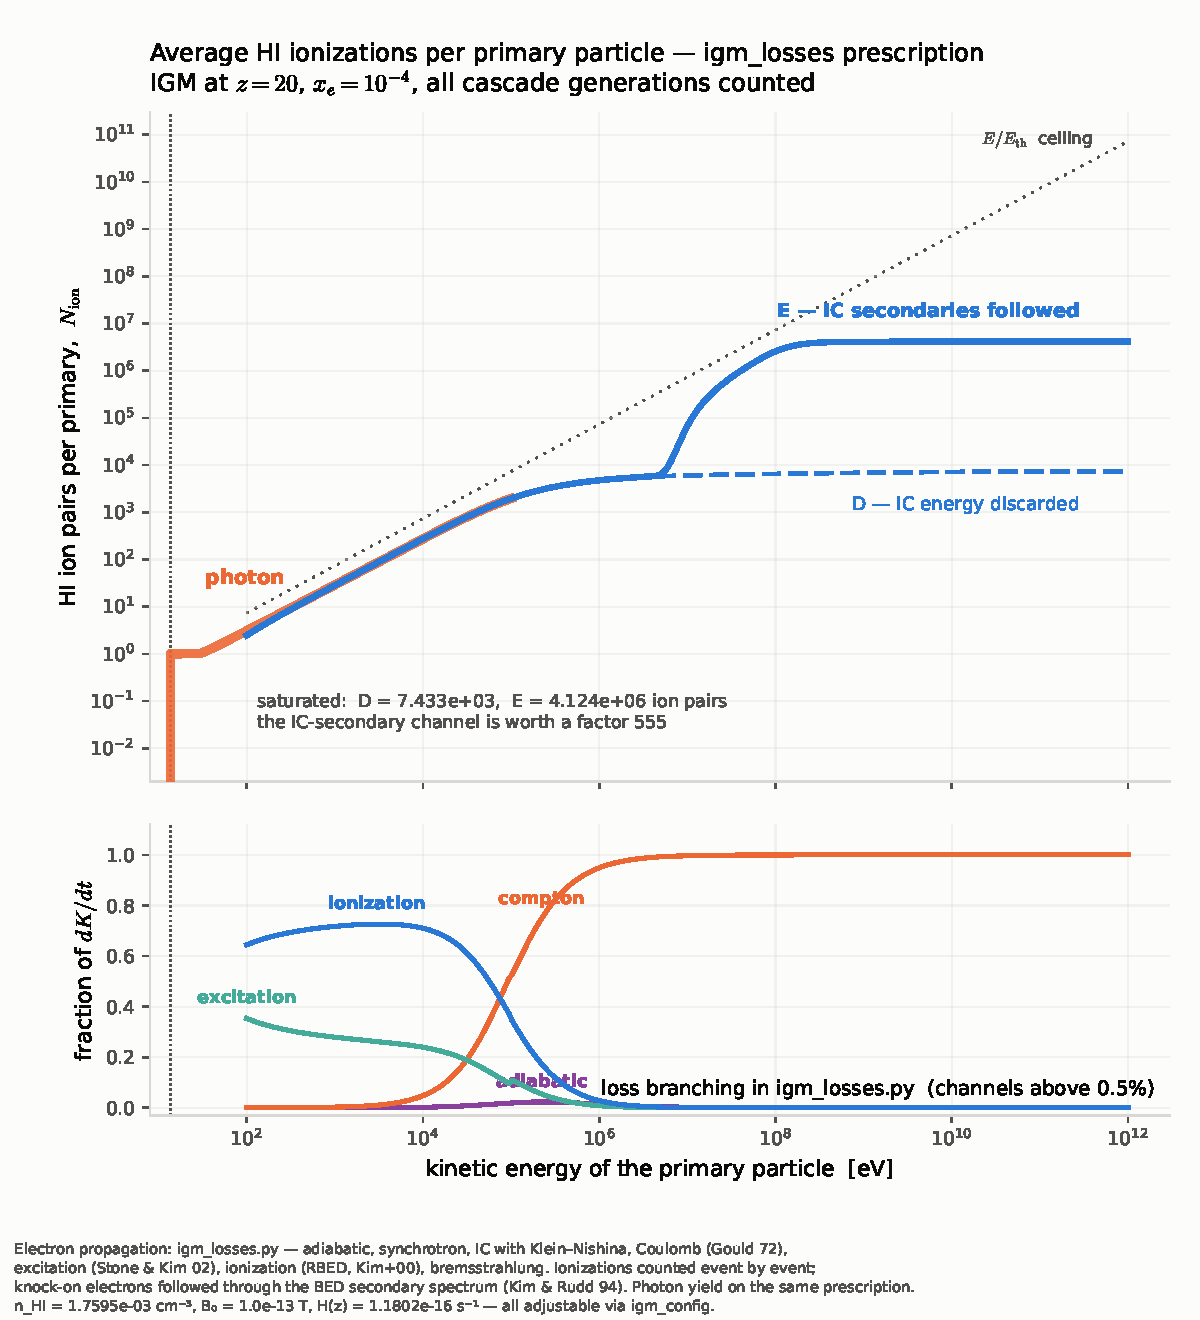
\includegraphics[width=0.70\textwidth]{ionization_yield_fig_igm_z20.pdf}
\caption{Figure~\ref{fig:yield} recomputed at $z=20$. Model~D saturates at
$7433$\src{N\_e\_loss\_sat\_z20} ion pairs against
$1.171\times10^{4}$\src{N\_e\_loss\_sat} at $z=10$, and model~E at
$4.124\times10^{6}$\src{N\_e\_loss\_ic\_sat\_z20} against
$4.911\times10^{6}$\src{N\_e\_loss\_ic\_sat}. Produced by
\texttt{ionization\_yield\_igm.py} through \texttt{run\_redshift\_suite.py}.}
\label{fig:z20yield}
\end{figure}
\paragraph{Reading Fig.~\ref{fig:z20yield}.} The same construction as
Fig.~\ref{fig:yield}, recomputed at $z=20$; only what \emph{changed} is stated
here. \emph{Conclusions.} (i) \textbf{Below $\sim10$~keV nothing moves} ---
every competing channel there is collisional and carries the same $n_{\rm HI}$,
which cancels from the branching ratio. (ii) \textbf{Above
$\sim100$~keV the yield falls}, because inverse Compton grows as $(1+z)^4$
against $(1+z)^3$ for the collisional channels: $E_{\rm crit}$ drops to
$8.896\times10^{4}$\src{E\_crit\_D\_eV\_z20}~eV and model~D loses a fraction
$0.3651$\src{loss\_sat\_drop\_frac\_z20} of its saturated yield. (iii)
\textbf{Model~E loses far less}, $0.1602$\src{Esat\_drop\_frac\_z20}, because
the energy inverse Compton takes is not destroyed --- so \textbf{the
IC-secondary channel matters \emph{more} at higher redshift}, its $E/D$ ratio
rising to $554.8$\src{lossic\_over\_loss\_sat\_z20}. (iv) \textbf{Adiabatic expansion
matters less}: its instantaneous share falls to
$0.02339$\src{adiabatic\_peak\_frac\_z20} and the energy it removes over the
whole cascade falls from $7.696$\src{Efrac\_adiabatic\_max\_pct}\% to
$1.849$\src{Efrac\_adiabatic\_max\_z20\_pct}\%, a factor
$4.162$\src{Efrac\_adiabatic\_drop\_z20}, because $H(z)$ grows only as
$(1+z)^{3/2}$ while the CMB energy density it competes with grows as $(1+z)^4$.


Three features of Fig.~\ref{fig:z20yield} are worth stating explicitly, because
they are the physics of the redshift change rather than an artefact of it.

\begin{enumerate}\itemsep3pt
\item \textbf{Below $\sim10$~keV nothing moves.} The yield at $10^3$~eV is
      $28.34$\src{N\_e\_loss\_1e+03\_z20} at $z=20$ against
      $28.35$\src{N\_e\_loss\_1e+03} at $z=10$, and the mean energy per ion pair
      at $1$~keV is $35.28$\src{W\_loss\_1keV\_z20}~eV against
      $35.27$\src{W\_loss\_1keV}~eV. Every competing channel there --- ionization,
      excitation, Coulomb --- is collisional and scales with the same
      $n_{\rm HI}$, so the density cancels from the branching ratio. This is a
      useful invariance: it is why $\zeta_e$ barely moves (below).
\item \textbf{Above $\sim100$~keV the yield falls.} Inverse Compton grows as
      $(1+z)^4$ while the collisional channels grow as $(1+z)^3$, so IC takes a
      larger share and fewer ionizations are produced per primary. The
      crossover energy $E_{\rm crit}$, where IC overtakes collisional losses,
      drops from $1.487\times10^{5}$\src{E\_crit\_D\_eV}~eV to
      $8.896\times10^{4}$\src{E\_crit\_D\_eV\_z20}~eV, and model~D loses a
      fraction $0.3651$\src{loss\_sat\_drop\_frac\_z20} of its saturated yield.
\item \textbf{The loss+IC route loses much less ---
      $0.1602$\src{Esat\_drop\_frac\_z20} --- and the secondary
      channel therefore matters \emph{more}.} The energy inverse Compton takes
      is not destroyed; it reappears as upscattered photons above $13.6$~eV.
      The ratio $E/D$ at saturation rises from
      $419.5$\src{lossic\_over\_loss\_sat} to $554.8$\src{lossic\_over\_loss\_sat\_z20}. The
      adiabatic channel moves the other way: its peak share of $dK/dt$ falls
      from $0.0929$\src{peakfrac\_adiabatic} to
      $0.02339$\src{adiabatic\_peak\_frac\_z20}, because $H(z)$ grows only as
      $(1+z)^{3/2}$ against the $(1+z)^4$ of the CMB.
\end{enumerate}

\begin{figure}[h]\centering
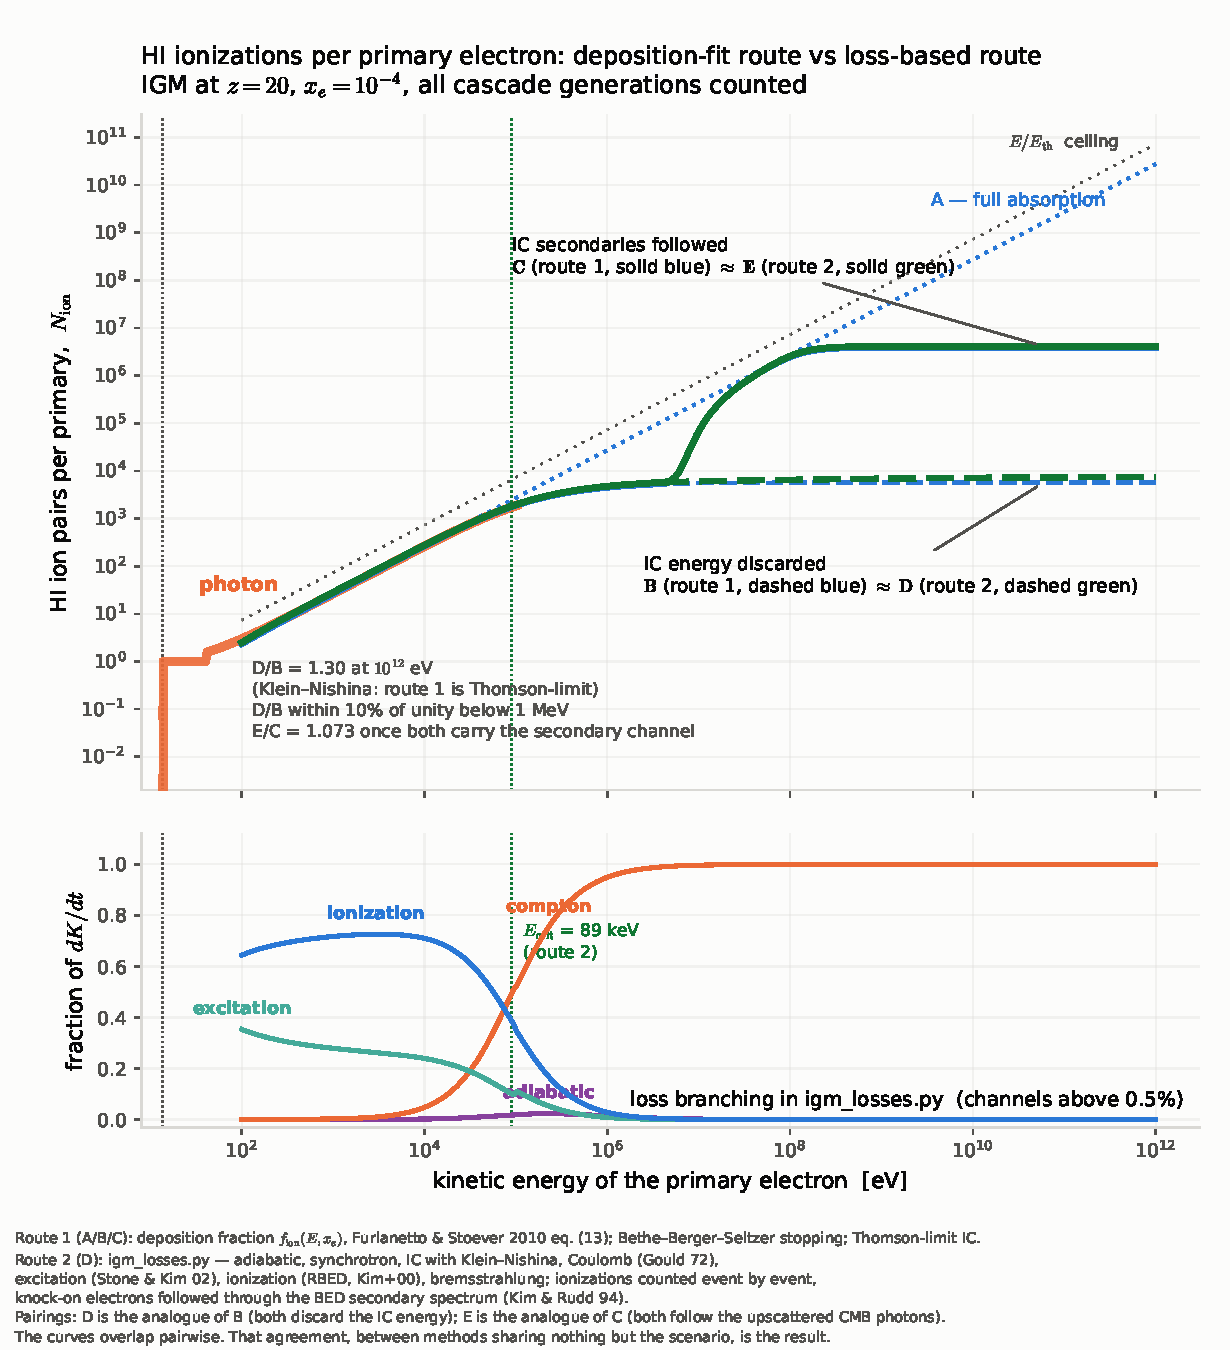
\includegraphics[width=0.88\textwidth]{yield_comparison_fig_z20.pdf}
\caption{The two-route cross-check at $z=20$. It survives the redshift change:
below 1~MeV the loss-based and deposition-fit routes agree to between
$1.047$\src{loss\_over\_ic\_min\_z20} and $1.102$\src{loss\_over\_ic\_max\_z20}, and with
the secondary channel carried on both sides the agreement at $10^{12}$~eV is
$1.073$\src{lossic\_over\_depfit\_1e12\_z20} --- the same $7\%$ as at $z=10$
($1.071$\src{lossic\_over\_depfit\_1e12}). Route~1 is not merely being re-evaluated here:
its cosmology is redshift-aware, so this is an independent recomputation.
Produced by \texttt{yield\_comparison.py}.}
\label{fig:z20validation}
\end{figure}
\paragraph{Reading Fig.~\ref{fig:z20validation}.} Fig.~\ref{fig:validation}
recomputed at $z=20$. \emph{Conclusion: the cross-check survives the redshift
change, which is the only thing this figure is asked to show.} Below 1~MeV the
two routes agree to between $1.047$\src{loss\_over\_ic\_min\_z20} and
$1.102$\src{loss\_over\_ic\_max\_z20}, and with the secondary channel on both sides
the agreement at $10^{12}$~eV is
$1.073$\src{lossic\_over\_depfit\_1e12\_z20} --- the same $7\%$ as at $z=10$. This is not a
re-evaluation of one route against a frozen other: route~1's cosmology is
redshift-aware, so both sides were independently recomputed.


\subsection{The competition at \texorpdfstring{$z=20$}{z = 20}}
\begin{figure}[h]\centering
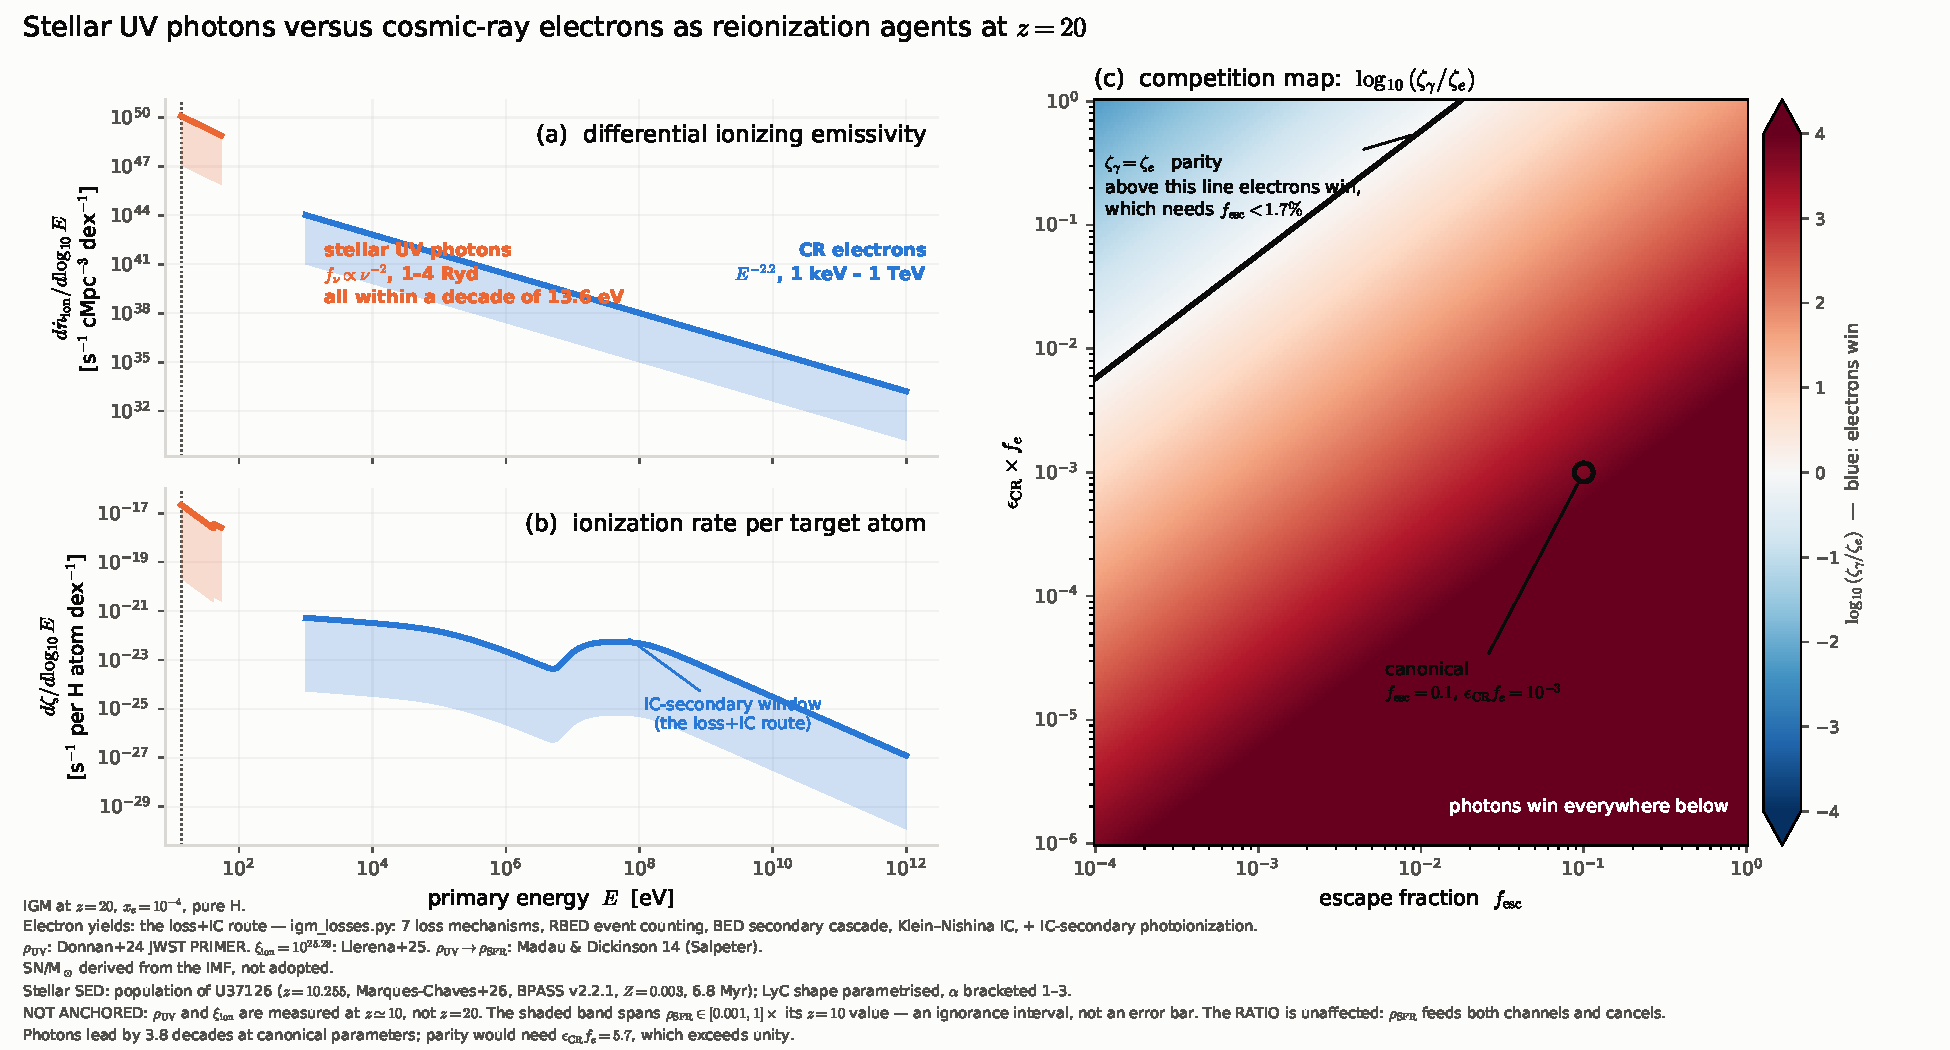
\includegraphics[width=\textwidth]{photon_vs_electron_fig1_z20.pdf}
\caption{Figure~\ref{fig:result} at $z=20$. Panels (a) and (b) carry the
$\rho_{\rm SFR}$ ignorance band; panel (c) does not need one. Produced by
\texttt{photon\_vs\_electron.py}.}
\label{fig:z20fig1}
\end{figure}
\paragraph{Reading Fig.~\ref{fig:z20fig1}.} Fig.~\ref{fig:result} at $z=20$.
Two things differ. First, \textbf{panels (a) and (b) now carry a shaded
ignorance band} spanning $\rho_{\rm SFR}\in[10^{-3},1]$ times its $z=10$ value,
because $\rho_{\rm UV}$ has never been measured at $z=20$; that band is an
assumption, not an error bar, and the absolute heights in those panels inherit
it. Second, \textbf{panel (c) needs no band at all} --- $\rho_{\rm SFR}$
normalises both channels and cancels from the ratio. \emph{Conclusion:} the
verdict is unchanged and slightly strengthened. The ratio rises to
$5748$\src{zeta\_ratio\_z20}, i.e.\ $3.760$\src{zeta\_ratio\_decades\_z20}
decades against $3.748$\src{zeta\_ratio\_decades} at $z=10$, and parity would
need $\epsilon_{\rm CR}f_e =
5.748$\src{eps\_cr\_fe\_crossover\_z20}, still above unity. The conclusions drawn
for panel~(a) of Fig.~\ref{fig:result} --- disjoint energy bands, heights not
comparable --- hold unchanged, since neither band depends on redshift.


\begin{itemize}\itemsep2pt
\item $\zeta_\gamma = 4.647\times10^{-18}\src{zeta\_gamma\_s\_z20}\
      \mathrm{s^{-1}}$ per \ion{H}{i} atom --- \emph{numerically identical} to
      $z=10$, and not by accident: the emissivity is comoving, the target count
      is comoving, and $\rho_{\rm UV}$ is held at its $z=10$ value because
      nothing better exists. This number carries the full ignorance of item~2
      above.
\item $\zeta_e = 8.085\times10^{-22}\src{zeta\_e\_s\_z20}\ \mathrm{s^{-1}}$ per
      atom, against $8.299\times10^{-22}$\src{zeta\_e\_s} at $z=10$: a fall of
      only $0.02586$\src{zeta\_e\_drop\_frac\_z20}, even though the saturated
      yield fell by $0.1602$\src{Esat\_drop\_frac\_z20}. The reason
      is item~1 above --- an $E^{-2.2}$ spectrum from $1$~keV is dominated by
      electrons of a few keV, where the yield is redshift-independent.
\item Ratio $5748$\src{zeta\_ratio\_z20}, i.e.\
      $3.760$\src{zeta\_ratio\_decades\_z20} decades, against
      $3.748$\src{zeta\_ratio\_decades} at $z=10$. Photons pull
      \emph{slightly further ahead}.
\item Parity would need
      $\epsilon_{\rm CR}f_e = 5.748$\src{eps\_cr\_fe\_crossover\_z20}, again
      above unity and therefore unreachable.
\end{itemize}

\begin{figure}[h]\centering
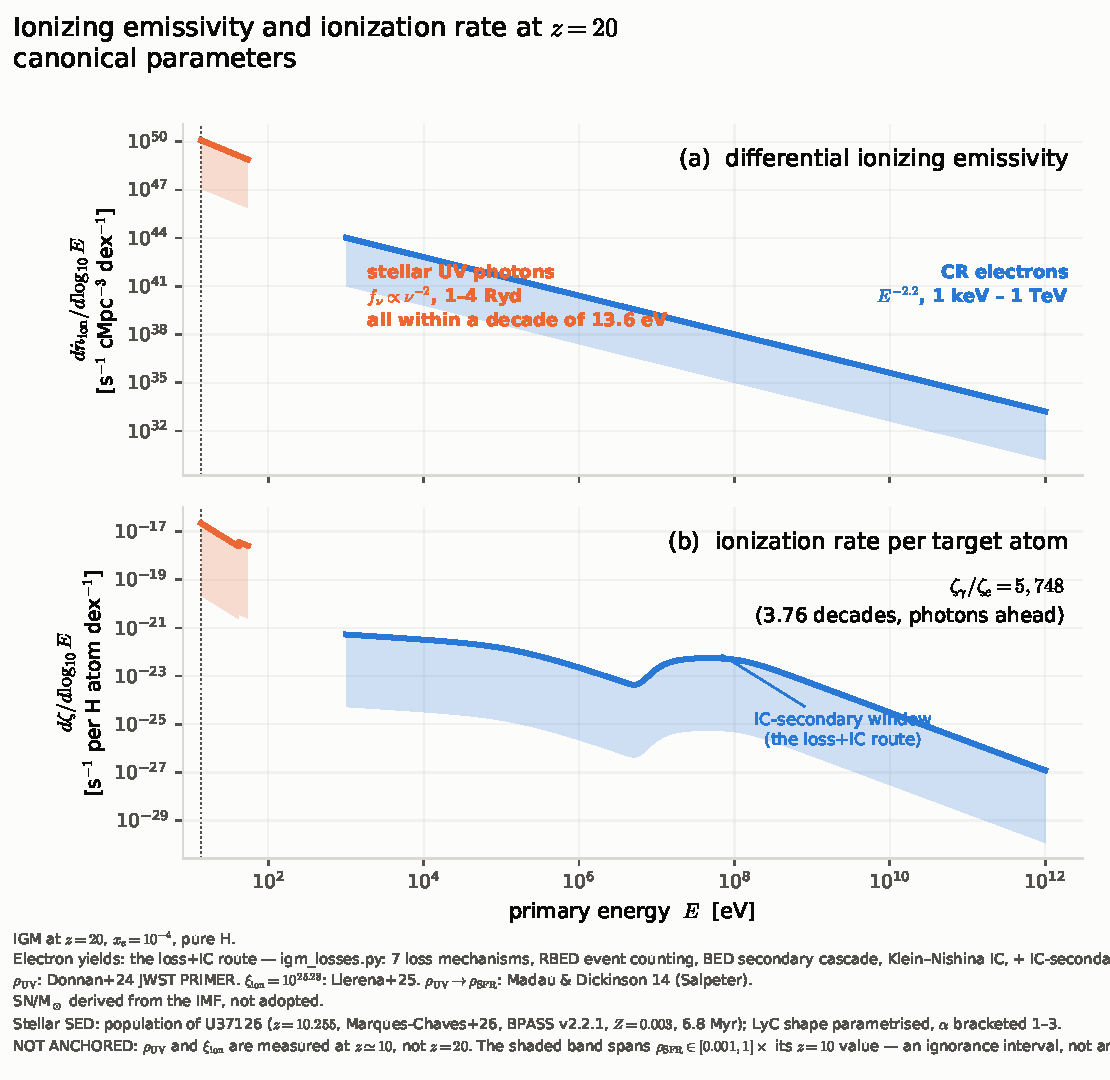
\includegraphics[width=0.68\textwidth]{photon_vs_electron_fig2a_z20.pdf}
\caption{Panels (a) and (b) alone at $z=20$, with the ignorance band.
Produced by \texttt{photon\_vs\_electron.py}.}
\label{fig:z20fig2a}
\end{figure}
\paragraph{Reading Fig.~\ref{fig:z20fig2a}.} Fig.~\ref{fig:2a} at $z=20$, with
the $\rho_{\rm SFR}$ ignorance band on both channels. It adds no conclusion
beyond Fig.~\ref{fig:z20fig1}; it is kept so that the two-panel layout exists at
both redshifts.


\begin{figure}[h]\centering
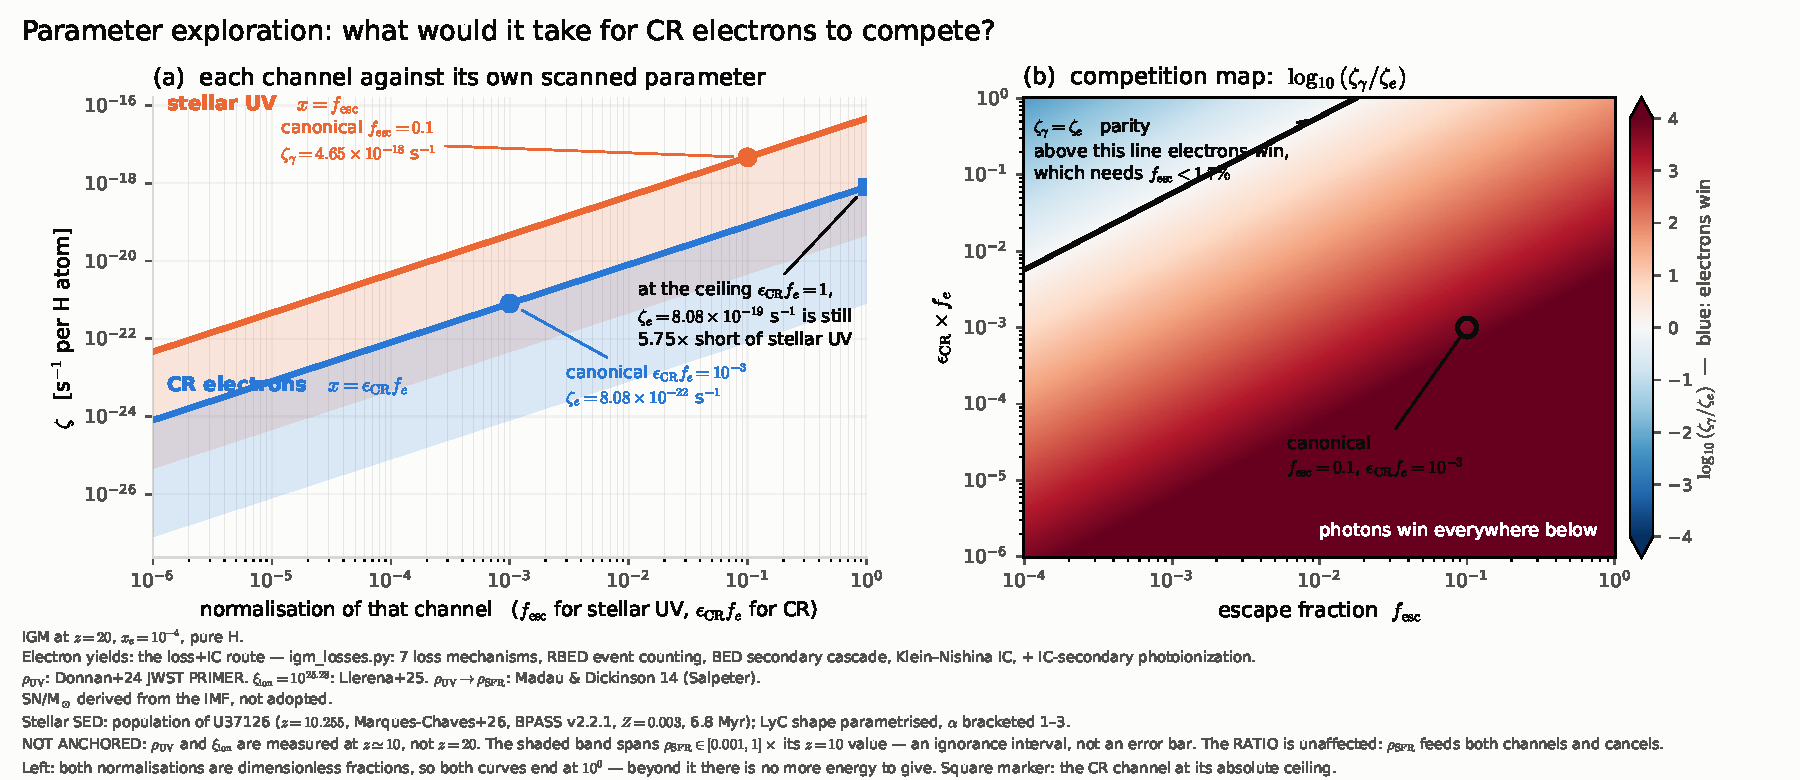
\includegraphics[width=0.96\textwidth]{photon_vs_electron_fig2b_z20.pdf}
\caption{Parameter exploration at $z=20$. The left panel's absolute axis
carries the ignorance band; the map on the right does not. Produced by
\texttt{photon\_vs\_electron.py}.}
\label{fig:z20fig2b}
\end{figure}
\paragraph{Reading Fig.~\ref{fig:z20fig2b}.} Fig.~\ref{fig:2b} at $z=20$. One
change matters: in the left panel the shaded band is \emph{no longer} the
published $\pm1\sigma$ on $\rho_{\rm UV}$ but the $\rho_{\rm SFR}$ ignorance
interval, applied to \emph{both} channels --- at a redshift where
$\rho_{\rm UV}$ has never been measured, drawing a measurement's error bar would
be worse than drawing nothing. \emph{Conclusion:} unchanged from
Fig.~\ref{fig:2b}. Both curves still end at $10^{0}$ because both
normalisations are still fractions bounded by unity, and at that ceiling the CR
channel remains short by $5.748$\src{eps\_cr\_fe\_crossover\_z20}.


\subsection{Ratio-only, at both redshifts}
Because the ratio is the one statement that survives without $\rho_{\rm UV}$,
it is also drawn on its own --- at $z=20$, and, at your request, at $z=10$ for
comparison.

\begin{figure}[h]\centering
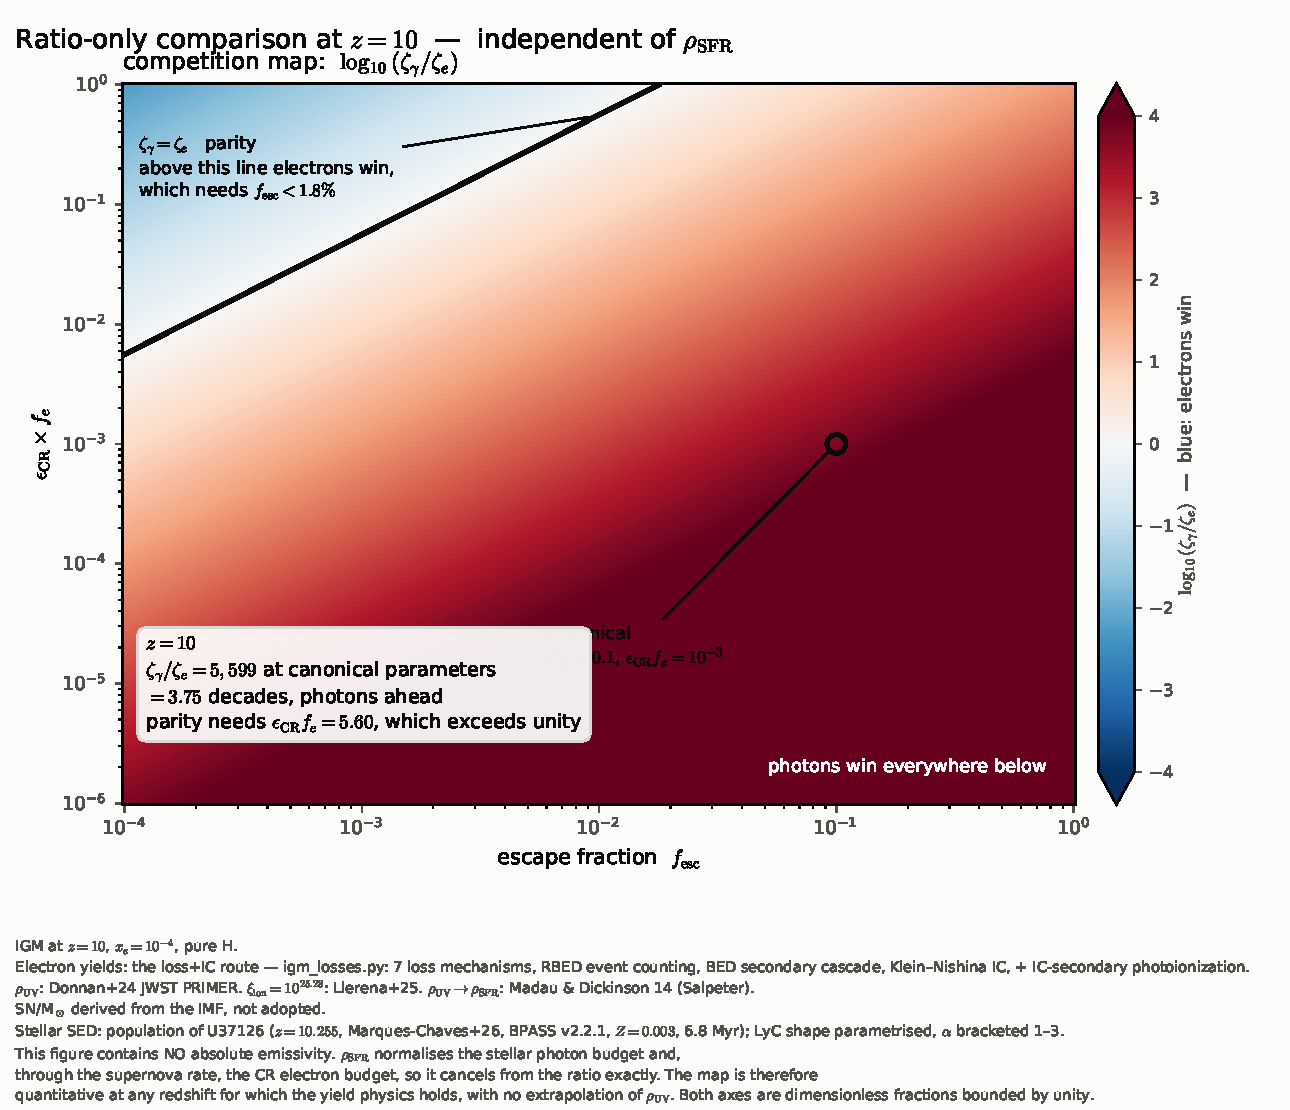
\includegraphics[width=0.62\textwidth]{photon_vs_electron_fig3.pdf}
\hfill
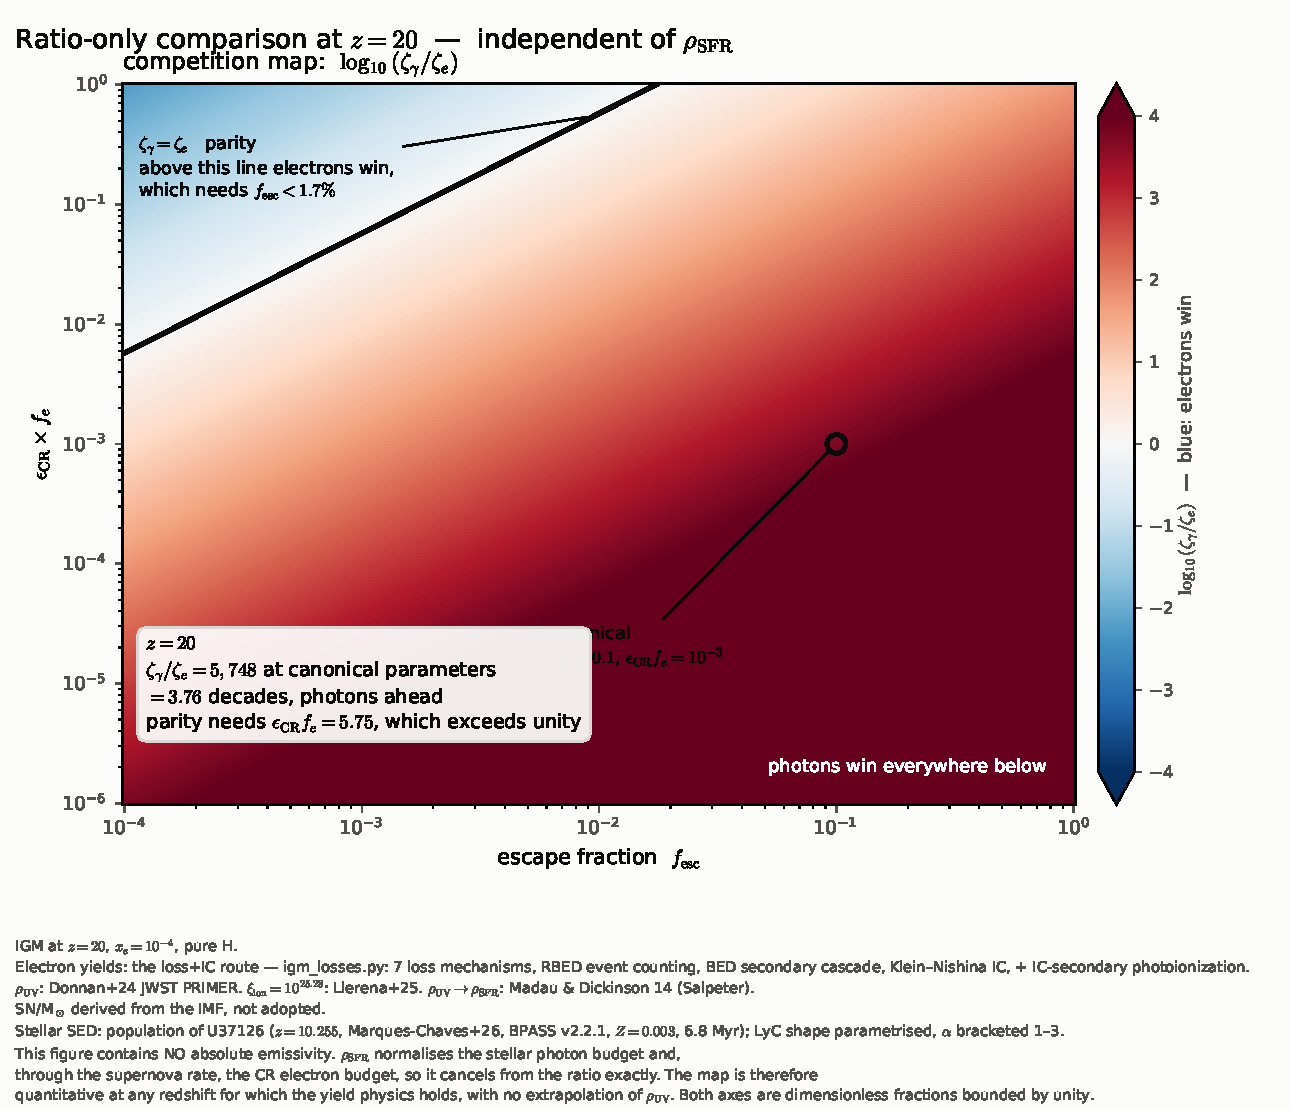
\includegraphics[width=0.62\textwidth]{photon_vs_electron_fig3_z20.pdf}
\caption{The competition map alone, at $z=10$ (upper) and $z=20$ (lower).
Nothing in either panel is extrapolated: both axes are dimensionless fractions
bounded by unity, and $\rho_{\rm SFR}$ has cancelled. The parity locus moves
from $f_{\rm esc}<1.786$\src{fesc\_parity\_pct\_z10}\% to
$f_{\rm esc}<1.740$\src{fesc\_parity\_pct\_z20}\%, i.e.\ hardly at all.
Produced by \texttt{photon\_vs\_electron.py}.}
\label{fig:z20ratio}
\end{figure}
\paragraph{Reading Fig.~\ref{fig:z20ratio}.} The competition map alone, at
$z=10$ (upper) and $z=20$ (lower). \emph{Why this figure exists:} it is the only
figure in the $z=20$ material with \textbf{nothing extrapolated in it}. Both
axes are dimensionless fractions bounded by unity, and $\rho_{\rm SFR}$ ---
which normalises the stellar photon budget and, through the supernova rate, the
cosmic-ray budget --- cancels exactly from the ratio. \emph{Conclusion:}
\textbf{the competition is almost independent of redshift.} The parity locus
moves only from $f_{\rm esc} < 1.786$\src{fesc\_parity\_pct\_z10}\% to
$f_{\rm esc} < 1.740$\src{fesc\_parity\_pct\_z20}\%, and the ratio from
$5599$\src{zeta\_ratio} to $5748$\src{zeta\_ratio\_z20}, a rise of just
$2.655$\src{zeta\_ratio\_rise\_z20\_pct}\% across a factor
$6.958$\src{n\_H\_ratio\_z20\_over\_z10} in density and a factor
$13.28$\src{U\_CMB\_ratio\_z20\_over\_z10} in CMB energy density. The reason is
the invariance found in Fig.~\ref{fig:z20yield} --- an $E^{-2.2}$ spectrum from
1~keV is dominated by few-keV electrons, where the yield does not depend on
redshift at all.


\subsection{What this does \emph{not} show}
\begin{enumerate}\itemsep2pt
\item The absolute $z=20$ rates are \textbf{not predictions}. Without a
      measured $\rho_{\rm UV}$ at that redshift they are the $z=10$
      normalisation carried sideways, with a factor-$10^{3}$ ignorance band
      attached by hand.
\item The ionizing-source population at $z=20$ is plausibly \emph{not} the
      $z\simeq10$ population: Population~III stars, a different IMF and a
      different $\xi_{\rm ion}$ are all live possibilities. None of that is
      modelled here. What is transferred is the \emph{yield physics}, which
      depends on the IGM and not on what made the particles.
\item $x_e=10^{-4}$ is held fixed at both redshifts. It is a choice, as at
      $z=10$.
\end{enumerate}

\clearpage
% ===========================================================================
\section{The reionization photon budget}\label{sec:budget}
% ===========================================================================
\S\ref{sec:norm} established \emph{which} clock the maintenance criterion uses.
This section derives the requirement algebraically, evaluates it, and tabulates
it over redshift and clumping factor. Produced by
\texttt{reionization\_budget.py}, 5/5 checks, registry
\texttt{provenance/reionization\_budget.json}; the algebra is verified with
\texttt{sympy} rather than asserted.

\subsection{Derivation}
\paragraph{(a) The balance, in photon-counting form.}
During reionization the IGM is optically thick to Lyman-continuum radiation, so
every escaping ionizing photon is absorbed somewhere and the supply term is the
full $\zeta$, not $\zeta(1-x)$. This is the form the budget literature uses
(Madau, Haardt \& Rees 1999). Per unit volume, with $x = n_{\rm HII}/n_{\rm H}$
and $n_e = \chi\,n_{\rm HII}$,
\begin{align}
  \text{supply:}\qquad        S &= \zeta\,n_{\rm H}, \\
  \text{recombinations:}\qquad R &= \alpha_B\,C\,n_e\,n_{\rm HII}
                                  = \alpha_B\,C\,\chi\,n_{\rm H}^2 x^2 ,
\end{align}
where $\chi = 1.08$ counts the electrons donated by singly ionized
helium~\cite{md14}. Dividing by $n_{\rm H}$,
\begin{equation}
  \frac{\mathrm{d}x}{\mathrm{d}t}
    = \zeta - \alpha_B\,C\,\chi\,n_{\rm H}\,x^2 .
  \label{eq:balance}
\end{equation}

\paragraph{(b) The maintenance condition is exactly
            \texorpdfstring{$\zeta t_{\rm rec}\ge1$}{zeta t_rec >= 1}.}
Ask what $\zeta$ holds a \emph{fully} ionized IGM in steady state: set
$\mathrm{d}x/\mathrm{d}t = 0$ and $x=1$ in eq.~\eqref{eq:balance},
\begin{equation}
  \zeta_{\rm crit} = \alpha_B\,C\,\chi\,n_{\rm H}
                   = \frac{1}{\langle t_{\rm rec}\rangle},
  \qquad
  \langle t_{\rm rec}\rangle
   = \bigl(\chi\,n_{\rm H}\,\alpha_B\,C\bigr)^{-1},
  \label{eq:zetacrit}
\end{equation}
which is \cite{md14} eq.~(24). The \texttt{sympy} residual
$\zeta_{\rm crit} - 1/\langle t_{\rm rec}\rangle$ is identically zero, so
\textbf{the recombination-time normalisation is not a convention: it is the
boundary at which ionizations can just hold the gas ionized.} Note that the
$x\to1$ limit is only meaningful in the photon-counting form: written with a
$\zeta(1-x)$ absorption term the supply vanishes at $x=1$ and the question
cannot be posed at all.

\paragraph{(c) Photons per atom.} Integrating eq.~\eqref{eq:balance}, each atom
needs one ionization plus one per recombination it suffers,
\begin{equation}
  N_{\rm req} = 1 + \int \frac{\mathrm{d}t}{\langle t_{\rm rec}\rangle} ,
  \qquad\text{and per Hubble time}\qquad
  \boxed{\;N_{\rm req} = 1 + \frac{t_H}{\langle t_{\rm rec}\rangle}
        = 1 + \frac{\chi\,n_{\rm H}(z)\,\alpha_B\,C}{H(z)}\;}
  \label{eq:Nreq}
\end{equation}

\paragraph{(d) Explicit redshift dependence.} With
$n_{\rm H}(z) = n_{{\rm H}0}(1+z)^3$ and, in matter domination,
$H(z)\to H_0\sqrt{\Omega_m}\,(1+z)^{3/2}$,
\begin{equation}
  N_{\rm req} - 1
   = \frac{\chi\,n_{{\rm H}0}\,\alpha_B\,C}{H_0\sqrt{\Omega_m}}\,(1+z)^{3/2} .
  \label{eq:Nreqscaling}
\end{equation}
So the excess over unity is \textbf{exactly linear in $C$} and rises as
$(1+z)^{3/2}$. Both are verified against the exact table below: the $C=12$
excess is $12.0000000000$\src{Nreq\_excess\_linearity\_C12\_over\_C1} times the
$C=1$ excess at $z=10$, and the excess grows by
$2.636$\src{Nreq\_excess\_ratio\_z20\_z10\_C1} from $z=10$ to $z=20$ against
the predicted $(21/11)^{3/2} =
2.638$\src{Nreq\_excess\_ratio\_predicted}, a $0.06\%$ departure that is
$\Lambda$ and radiation in the exact Planck-18 $H(z)$ which the power law omits.
\textbf{The physical content of eq.~\eqref{eq:Nreqscaling} is that the
requirement gets harder at higher redshift}, because the gas gets denser
($t_{\rm rec}\propto(1+z)^{-3}$) faster than the clock gets short
($t_H\propto(1+z)^{-3/2}$).

\subsection{Inputs}
\begin{center}\small
\begin{tabular}{lll}
\hline
quantity & value & source \\
\hline
$\chi$ & $1.08$\src{chi\_He} & \cite{md14} eq.~(24); electrons from singly ionized He \\
$\alpha_B(2\times10^4~\mathrm{K})$ & $1.430\times10^{-13}$\src{alpha\_B\_2e4K}~cm$^3$s$^{-1}$
  & Osterbrock \& Ferland 2006, Table 2.1; $T$ as assumed by \cite{md14} \\
$n_{{\rm H}0}$ & $1.900\times10^{-7}$\src{n\_H0\_cm3}~cm$^{-3}$
  & this work's harmonised $n_{\rm H}(z{=}10)/11^3$ \\
$H(z)$ & Planck 18 & \texttt{astropy}; the complete $H(z)$, radiation included \\
$C_{\rm IGM}(z)$ & $1 + 43\,z^{-1.71}$ & Pawlik et al.\ 2009, via \cite{md14} \\
\hline
\end{tabular}
\end{center}
As a check that these inputs are the ones \cite{md14} used, eq.~\eqref{eq:zetacrit}
evaluated at $(1+z)/7 = 1$ with $C_{\rm IGM}=1$ returns
$3.149$\src{t\_rec\_z6\_C1\_Gyr}~Gyr against the $3.2$~Gyr printed in their
eq.~(24) --- agreement to $1.6\%$, recomputed from our own $n_{{\rm H}0}$ rather
than quoted.

\subsection{Required photons per hydrogen atom, in both normalisations}
Eq.~\eqref{eq:Nreq} is the requirement \emph{per Hubble time}. The same
requirement per \emph{recombination} time is the identical statement with the
clock swapped,
\begin{equation}
  N_{\rm req}^{(t_{\rm rec})}
    = N_{\rm req}^{(t_H)}\times\frac{\langle t_{\rm rec}\rangle}{t_H}
    = \Bigl(1+\frac{t_H}{\langle t_{\rm rec}\rangle}\Bigr)
      \frac{\langle t_{\rm rec}\rangle}{t_H}
    = 1 + \frac{\langle t_{\rm rec}\rangle}{t_H} ,
  \label{eq:Nreqtrec}
\end{equation}
so the two tables below are mirror images of one another and contain exactly the
same physics. Read term by term they say different things, and that is the point
of the question: in eq.~\eqref{eq:Nreq} the ``$1$'' is the single initial
ionization and the varying term counts recombinations, whereas in
eq.~\eqref{eq:Nreqtrec} the ``$1$'' \emph{is} the recombination --- exactly one
per recombination time, by construction --- and the varying term is that initial
ionization amortised over one recombination time. Verified across all nine
cells: $N_{\rm req}^{(t_{\rm rec})} - \langle t_{\rm rec}\rangle/t_H = 1$ to
$2\times10^{-16}$.

\begin{table}[h]\centering\footnotesize
\setlength{\extrarowheight}{2pt}
\setlength{\tabcolsep}{4pt}
\resizebox{\textwidth}{!}{%
\begin{tabular}{|c|c|c|c|c|c|c|}
\hline
$z$ & $t_H$ [Gyr] & $n_{\rm H}$ [cm$^{-3}$]
    & $C = 1$ & $C = 3$ & $C = 12$ & $C_{\rm IGM}(z)$ \\
\hline
$20$ & $0.2685$\src{t\_H\_Gyr\_z20} & $1.7595\times10^{-3}$\src{n\_H\_cm3\_z20}
     & $3.302$\src{Nreq\_z20\_C1} & $7.907$\src{Nreq\_z20\_C3}
     & $28.63$\src{Nreq\_z20\_C12}
     & $3.892$\src{Nreq\_z20\_CMD14} \\
\hline
$10$ & $0.7086$\src{t\_H\_Gyr\_z10} & $2.5287\times10^{-4}$\src{n\_H\_cm3\_z10}
     & $1.873$\src{Nreq\_z10\_C1} & $3.620$\src{Nreq\_z10\_C3}
     & $11.48$\src{Nreq\_z10\_C12}
     & $2.606$\src{Nreq\_z10\_CMD14} \\
\hline
$5.5$ & $1.556$\src{t\_H\_Gyr\_z5p5} & $5.2175\times10^{-5}$\src{n\_H\_cm3\_z5p5}
     & $1.396$\src{Nreq\_z5p5\_C1} & $2.187$\src{Nreq\_z5p5\_C3}
     & $5.748$\src{Nreq\_z5p5\_C12}
     & $2.318$\src{Nreq\_z5p5\_CMD14} \\
\hline
\end{tabular}}
\caption{\textbf{Hubble-time normalisation.}
$N_{\rm req}^{(t_H)} = 1 + t_H/\langle t_{\rm rec}\rangle$,
eq.~\eqref{eq:Nreq} --- the ionizing photons each hydrogen atom must receive
\emph{per Hubble time} for the IGM to stay ionized. The ``$1$'' is the initial
ionization; everything above it is recombinations. This table contains no
$\rho_{\rm UV}$ and no star-formation history, which is why it is quotable at
$z=5.5$ where this work has no measured source normalisation.}
\label{tab:budget}
\end{table}

\begin{table}[h]\centering\footnotesize
\setlength{\extrarowheight}{2pt}
\setlength{\tabcolsep}{4pt}
\resizebox{\textwidth}{!}{%
\begin{tabular}{|c|c|c|c|c|c|c|}
\hline
$z$ & $t_H$ [Gyr] & $n_{\rm H}$ [cm$^{-3}$]
    & $C = 1$ & $C = 3$ & $C = 12$ & $C_{\rm IGM}(z)$ \\
\hline
$20$ & $0.2685$\src{t\_H\_Gyr\_z20} & $1.7595\times10^{-3}$\src{n\_H\_cm3\_z20}
     & $1.434$\src{NreqTrec\_z20\_C1} & $1.145$\src{NreqTrec\_z20\_C3}
     & $1.036$\src{NreqTrec\_z20\_C12}
     & $1.346$\src{NreqTrec\_z20\_CMD14} \\
\hline
$10$ & $0.7086$\src{t\_H\_Gyr\_z10} & $2.5287\times10^{-4}$\src{n\_H\_cm3\_z10}
     & $2.145$\src{NreqTrec\_z10\_C1} & $1.382$\src{NreqTrec\_z10\_C3}
     & $1.095$\src{NreqTrec\_z10\_C12}
     & $1.623$\src{NreqTrec\_z10\_CMD14} \\
\hline
$5.5$ & $1.556$\src{t\_H\_Gyr\_z5p5} & $5.2175\times10^{-5}$\src{n\_H\_cm3\_z5p5}
     & $3.527$\src{NreqTrec\_z5p5\_C1} & $1.842$\src{NreqTrec\_z5p5\_C3}
     & $1.211$\src{NreqTrec\_z5p5\_C12}
     & $1.759$\src{NreqTrec\_z5p5\_CMD14} \\
\hline
\end{tabular}}
\caption{\textbf{Recombination-time normalisation.}
$N_{\rm req}^{(t_{\rm rec})} = 1 + \langle t_{\rm rec}\rangle/t_H$,
eq.~\eqref{eq:Nreqtrec} --- the same requirement counted \emph{per recombination
time}. Here the ``$1$'' is the recombination itself, so the entries subtract to
$\langle t_{\rm rec}\rangle/t_H$ exactly and the table doubles as the conversion
factor between the two normalisations. \emph{Note the trends invert:} the
$C$ and $z$ dependence that made Table~\ref{tab:budget} rise now makes this one
fall toward unity, because a larger $C$ or a higher $z$ shortens
$\langle t_{\rm rec}\rangle$ and therefore shrinks the clock the count is taken
against. The last column again uses
$C_{\rm IGM} = 1+43z^{-1.71}$, i.e.\ $1.256$, $1.838$ and $3.330$ at
$z = 20$, $10$ and $5.5$ respectively.}
\label{tab:budgettrec}
\end{table}

\subsection{Reading the tables}
\begin{enumerate}\itemsep3pt
\item \textbf{The requirement is never one photon per atom.} Only in the
      idealised $C=1$, low-$z$ corner does it approach it
      ($1.396$\src{Nreq\_z5p5\_C1} at $z=5.5$). Everywhere else recombinations
      dominate the budget: at $z=20$ with $C=12$ each atom must be ionized
      $28.63$\src{Nreq\_z20\_C12} times per Hubble time.
\item \textbf{Clumping is the strongest lever.} $N_{\rm req}-1$ is exactly
      linear in $C$, so the factor-$12$ span of the columns costs a factor $12$
      in the recombination term. $C$ is a simulation-calibrated quantity, not a
      measurement, so it is the dominant systematic in any reionization budget
      --- including this one.
\item \textbf{The two tables invert, and that is the whole content of the
      question.} In the Hubble-time normalisation the requirement \emph{rises}
      with $C$ and with $z$; in the recombination-time normalisation it
      \emph{falls} toward unity. Nothing physical changes between them --- the
      ratio of any two corresponding cells is exactly
      $\langle t_{\rm rec}\rangle/t_H$. What changes is which term is held
      fixed: eq.~\eqref{eq:Nreq} pins the initial ionization at $1$ and lets the
      recombination count vary, eq.~\eqref{eq:Nreqtrec} pins the recombination
      count at $1$ and lets the amortised initial ionization vary.
      \textbf{The recombination-time form is the one to quote for a maintenance
      statement}, precisely because it normalises away the quantity the
      criterion is about and leaves a number to be compared with unity.
\item \textbf{Redshift works against you} (in the Hubble-time form). Between
      $z=5.5$ and $z=20$ the
      requirement rises by a factor
      $2.366$\src{Nreq\_rise\_z5p5\_to\_z20\_C1} at $C=1$,
      $3.615$\src{Nreq\_rise\_z5p5\_to\_z20\_C3} at $C=3$ and
      $4.980$\src{Nreq\_rise\_z5p5\_to\_z20\_C12} at $C=12$, following
      eq.~\eqref{eq:Nreqscaling}. With the redshift-dependent $C_{\rm IGM}$ the
      rise is milder,
      $1.679$\src{Nreq\_rise\_z5p5\_to\_z20\_CMD14}, because the clumping factor
      itself falls with redshift and partly offsets the density.
      Reionization is therefore harder to sustain early, which is the
      quantitative content of the statement that it \emph{completes} near
      $z\approx6$ rather than beginning there.
\item \textbf{Against this, what the two channels supply.} At $z=10$ with the
      \cite{md14} clumping, the requirement is
      $2.606$\src{Nreq\_z10\_CMD14} and the stellar channel supplies
      $\zeta_\gamma t_H = 0.1039$\src{zeta\_gamma\_tH}, short by
      $25.07$\src{reion\_shortfall\_factor}; the cosmic-ray channel is short by
      $1.404\times10^{5}$\src{reion\_shortfall\_factor\_CR}. The requirement
      here, $2.606$\src{Nreq\_z10\_CMD14}, is computed by
      \texttt{reionization\_budget.py} and by
      \texttt{photon\_vs\_electron.py} through independent code paths that
      agree to $0$ in double precision --- a cross-check, not a restatement.
      Both shortfalls
      scale inversely with the supply and linearly with $C$, so no choice of
      $C$ in Table~\ref{tab:budget} rescues the cosmic-ray channel: even at
      $C=1$, $z=5.5$ --- the most permissive cell in the table --- it remains
      short by more than four orders of magnitude.
\item \textbf{What this does not say.} $N_{\rm req}$ is a \emph{maintenance}
      requirement evaluated at the mean density with a single clumping factor.
      It is not a reionization history: no radiative transfer, no ionized-bubble
      topology, no spatial fluctuation in $C$, and no helium beyond the $\chi$
      factor. The caveats of \S\ref{sec:notchecked} apply unchanged.
\end{enumerate}

\clearpage
% ===========================================================================
\section{Does the IMF change the answer?}\label{sec:imf}
% ===========================================================================
The competition ratio of \S\ref{sec:result} reduces to eight numbers, and three
of them --- $\xi_{\rm ion}$, $K_{\rm UV}$ and the supernova yield per solar
mass --- are all functions of the stellar initial mass function. Treating them
as independent inputs with independent uncertainties, as the error budget of
\S\ref{sec:result} does, is therefore wrong in principle. This section tests
how much it matters in practice by recomputing everything with a top-heavy IMF.

\subsection{The fiducial top-heavy IMF}
Jeong, Jeon, Song \& Bromm~\cite{jeong25}, their eq.~(2), adopt
\begin{equation}
  \xi(m) = \frac{\mathrm{d}N}{\mathrm{d}m} = \xi_0\,m^{-\alpha},
  \qquad \alpha = 1.3, \qquad 1\,M_\odot \le m \le 100\,M_\odot ,
  \label{eq:imf_th}
\end{equation}
explicitly \emph{for Population~II stars}, in galaxies forming at $z=10$ ---
this calculation's population and redshift. The physical motivation is a raised
temperature floor in low-metallicity gas radiatively coupled to a CMB at
$T = 2.73(1+z)$~K, which lifts the Jeans mass and hence the characteristic
stellar mass~\cite{larson98}. It is the same functional form as the Salpeter
law~\cite{salpeter} already in use, so it substitutes into the supernova-rate
integral with no change of machinery: only $\alpha$ and $m_{\min}$ move.

\subsection{What the IMF moves, and what it does not}
\paragraph{The stellar channel does not move at all.} $\zeta_\gamma$ depends on
the IMF only through $\xi_{\rm ion}$, and $\xi_{\rm ion}$ is \emph{measured} ---
a line-to-continuum ratio~\cite{llerena25} that already carries whatever IMF
nature chose. $\rho_{\rm UV}$ is likewise an observation. Changing the IMF we
\emph{assume} does not change what was \emph{observed}, so both panels (a) and
(b) of Fig.~\ref{fig:imf} carry a single stellar curve.

\paragraph{The supernova rate per unit mass rises.} Integrating
eq.~\eqref{eq:imf_th} above $8\,M_\odot$ gives
$0.02754$\src{snM\_topheavy}~$M_\odot^{-1}$ against
$0.007422$\src{snM\_salpeter} for Salpeter --- a factor
$3.711$\src{f\_snM}, or one supernova per $36\,M_\odot$ instead of one per
$135\,M_\odot$.

\paragraph{But the UV output per unit mass rises almost identically.}
\cite{jeong25} give the conversion factor for both cases: $K_{\rm UV}$ for
their Chabrier/Salpeter baseline, and $\eta_{\rm UV} =
3.57\times10^{28}$\src{eta\_UV\_topheavy}~erg\,s$^{-1}$Hz$^{-1}$/($M_\odot$yr$^{-1}$)
for the top-heavy case, i.e.\ a factor
$0.2801$\src{K\_ratio\_jeong} on $K_{\rm UV}$. Applying that ratio to this
work's Salpeter value gives $K_{\rm UV} =
3.221\times10^{-29}$\src{K\_topheavy} against
$1.150\times10^{-28}$\src{K\_salpeter}.

\paragraph{The two nearly cancel.} What enters $\zeta_e$ is the
\emph{product} $K_{\rm UV}\times(\mathrm{SN}/M_\odot)$, and it changes by only
$1.040$\src{f\_product}. The reason is physical rather than coincidental:
$\rho_{\rm UV}$ is observed, not $\rho_{\rm SFR}$. A top-heavy IMF makes more
supernovae per unit mass, but it also makes more ultraviolet light per unit
mass, so the star-formation rate \emph{inferred} from a fixed observed
$\rho_{\rm UV}$ falls by almost the same factor that the supernova yield rises.
\textbf{The supernova rate per unit observed UV luminosity is close to
IMF-invariant}, and that --- not the supernova rate per unit mass --- is what
this calculation actually needs.

\begin{figure}[h]\centering
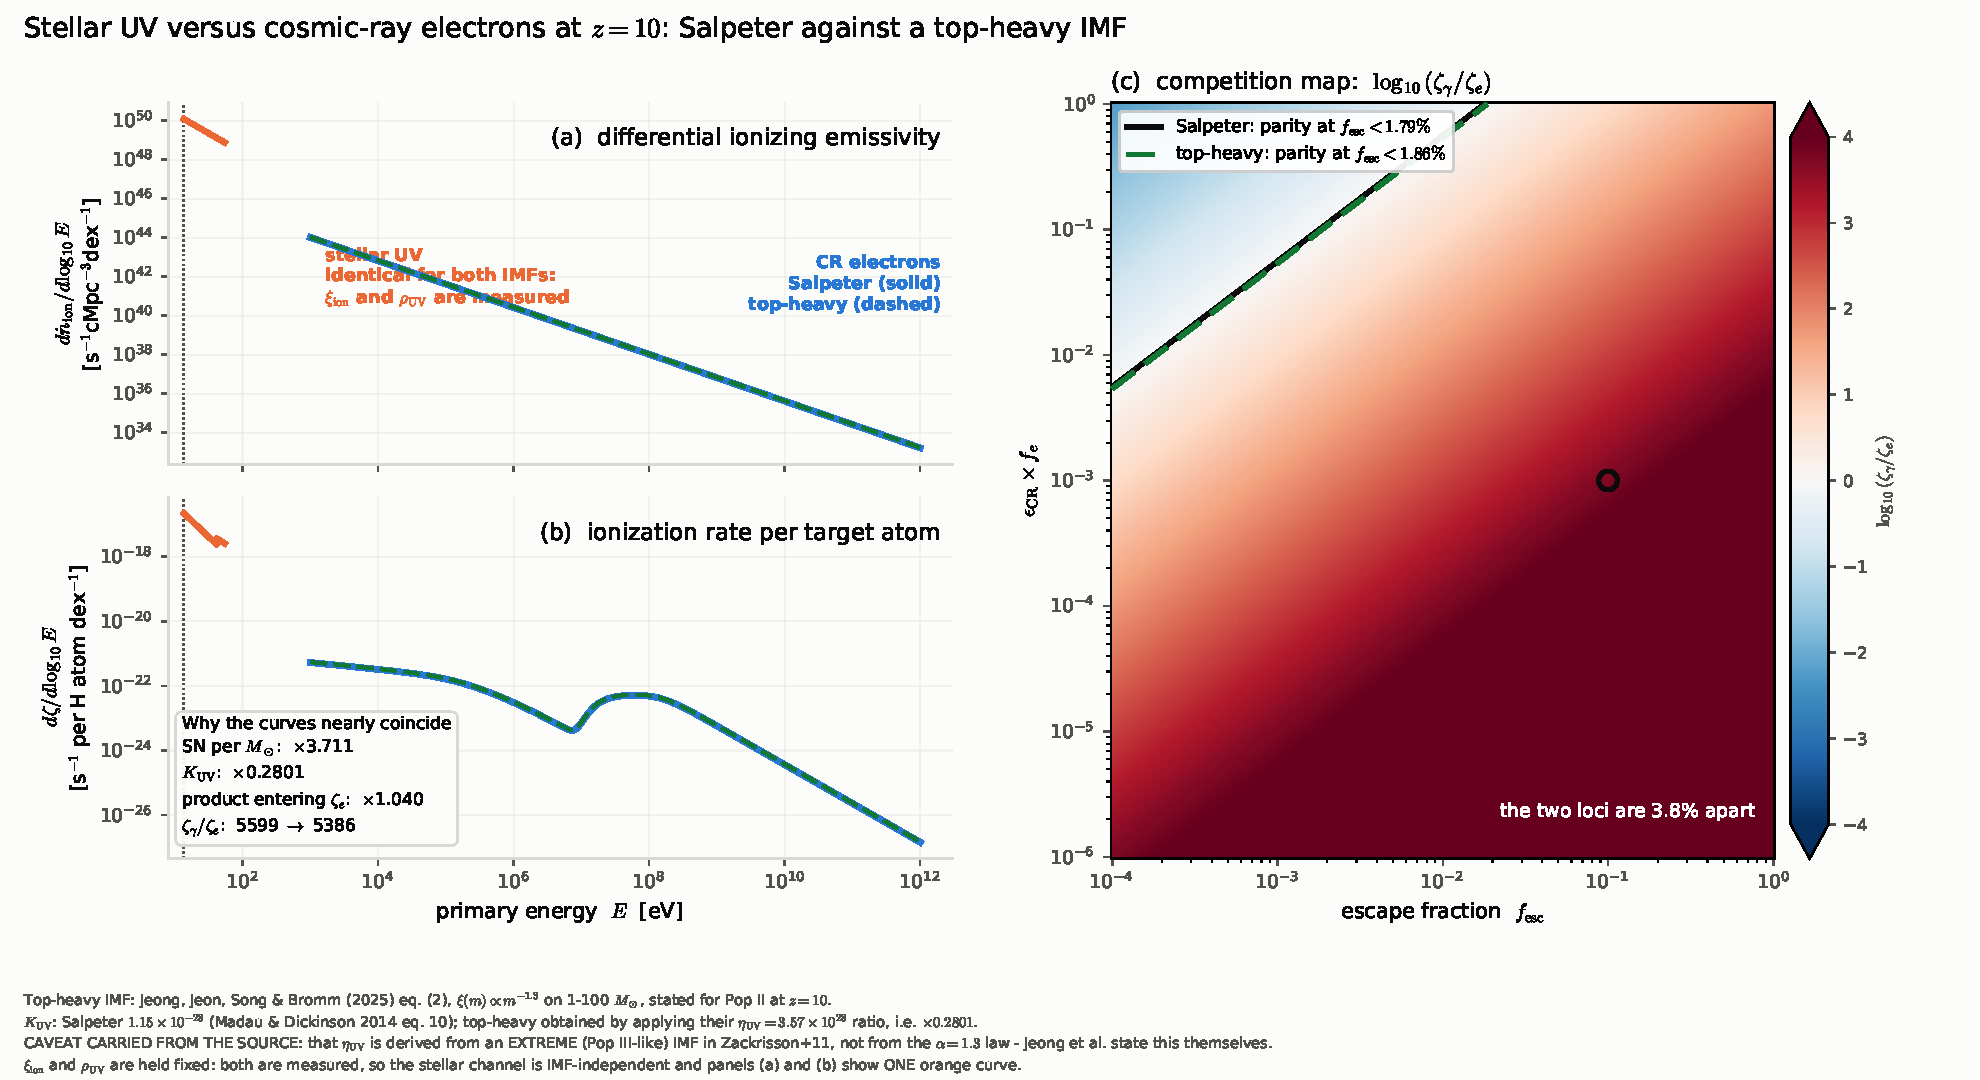
\includegraphics[width=\textwidth]{imf_comparison_fig.pdf}
\caption{Fig.~\ref{fig:result} recomputed for two initial mass functions:
Salpeter (solid) and the top-heavy law of eq.~\eqref{eq:imf_th} (dashed).
Produced by \texttt{imf\_comparison.py}.}
\label{fig:imf}
\end{figure}

\paragraph{Reading Fig.~\ref{fig:imf}.} Panels (a) and (b) plot the same two
quantities as Fig.~\ref{fig:result}, with one stellar curve and two CR curves.
\emph{The conclusion is the overlap.} $\zeta_e$ moves from
$8.299\times10^{-22}$\src{zeta\_e\_salpeter} to
$8.627\times10^{-22}$\src{zeta\_e\_topheavy}~s$^{-1}$ per atom, the ratio from
$5599$\src{ratio\_salpeter} to $5386$\src{ratio\_topheavy} --- the top-heavy
value is $0.9620$\src{f\_ratio} of the Salpeter one --- and in panel (c) the two
parity loci sit within a line width of one another, moving only from
$f_{\rm esc} < 1.79\%$ to $f_{\rm esc} < 1.86\%$. Parity would still require
$\epsilon_{\rm CR}f_e = 5.386$\src{eps\_parity\_topheavy}, above unity.
\textbf{Replacing the IMF with a drastically top-heavy one --- removing the
entire $0.1$--$1\,M_\odot$ reservoir and flattening the slope by a full unit ---
changes the headline result by under $4\%$.}

\subsection{Where \texorpdfstring{$K_{\rm UV}$}{K\_UV} comes from, and why two
            values are in circulation}\label{sec:kuv}
Two different Salpeter $K_{\rm UV}$ appear above, both attributed
to~\cite{md14}: this work's $1.15\times10^{-28}$ and the $1.00\times10^{-28}$
quoted by~\cite{jeong25}. They are not in conflict, and the reason is worth
recording.

$K_{\rm UV}$ is defined by \cite{md14} eq.~(10), ${\rm SFR} = K_{\rm UV}\,
L_\nu({\rm FUV})$, and is computed with a population-synthesis code for an
assumed IMF, star-formation history, age and metallicity. It is therefore not a
measurement but a \emph{model output}, and it varies with all four. Their
Figure~3 shows exactly that variation, and their text states that age and
metallicity ``counterbalance each other to a certain degree, so that
$K_{\rm FUV}(z)$ changes by less than $20\%$''.
\begin{itemize}\itemsep2pt
\item \textbf{$1.15\times10^{-28}$} is the value \cite{md14} \emph{adopt} for
      the review: in their words, ``a compromise value based on the
      evolutionary scenario from Figure~3'', chosen to be representative of the
      peak era of cosmic star formation. This is the number used throughout
      this document.
\item \textbf{$1.00\times10^{-28}$} is a \emph{point} on that same figure, read
      off at $\log_{10}Z_\star/Z_\odot = -1.0$, computed with
      \textsc{fsps} for a Salpeter IMF and constant SFR. That is the value
      \cite{jeong25} take, appropriate to their low-metallicity simulations.
\end{itemize}
The $15\%$ between them is therefore the metallicity dependence of a synthesis
model, and it sits inside the $20\%$ spread \cite{md14} themselves quote. For
scale, the widely used Kennicutt (1998) value, $1.4\times10^{-28}$, is $20\%$
\emph{larger} than the one adopted here --- \cite{md14} discuss this
explicitly. \textbf{Only the ratio between the two IMFs is taken from
\cite{jeong25}}; the Salpeter anchor remains this work's own, so the Salpeter
curve in Fig.~\ref{fig:imf} is identical to that in Fig.~\ref{fig:result}.

\paragraph{What the borrowed conversion actually was.} Chasing
\cite{jeong25}'s $\eta_{\rm UV}$ to its source, Zackrisson et
al.~\cite{zackrisson11}, shows the substitution is looser than their own caveat
admits. That paper's IMFs are Kroupa~(2001) for Pop~I/II, a Raiter et al.\
log-normal with $M_c = 10\,M_\odot$ for Pop~III.2, and --- the ``extreme
top-heavy'' one --- a Schaerer~(2002) power law of slope
$\alpha = 2.35$ over $50$--$500\,M_\odot$ at \emph{zero} metallicity. That is
the Salpeter slope; it is top-heavy by mass \emph{range} alone, and it shares no
parameter with the $\alpha = 1.3$, $1$--$100\,M_\odot$ Pop~II law it was lent
to. Neither $\xi_{\rm ion}$ nor $K_{\rm UV}$ is tabulated anywhere in
\cite{zackrisson11}, for any IMF.

\subsection{What this test does not establish}
\begin{enumerate}\itemsep2pt
\item \textbf{The top-heavy $\eta_{\rm UV}$ is borrowed.} \cite{jeong25} derive
      it from ``extreme top-heavy IMF values'' in Zackrisson et
      al.~\cite{zackrisson11} --- a Population~III-like IMF, not their own
      $\alpha=1.3$ law --- and caution that ``the functional IMFs of both values
      are not perfectly suited to our specific IMFs''. That caveat is inherited
      here in full. A $K_{\rm UV}$ computed for eq.~\eqref{eq:imf_th} itself
      would be preferable and does not exist in the sources consulted.
\item \textbf{The cancellation is not a theorem.} It holds for this pair of
      IMFs and this pair of conversion factors. Its near-exactness
      ($4\%$) should be read as suggestive, not as a proof that the result is
      IMF-independent in general.
\item \textbf{$\xi_{\rm ion}$ was held fixed by choice}, on the argument that it
      is an observable. That is right if the question is ``what if the IMF we
      \emph{assume} for the CR channel is wrong''. It would be wrong if the
      question were ``what would a fully synthetic top-heavy population look
      like'', in which case $\xi_{\rm ion}$ would have to be recomputed too.
\end{enumerate}


\clearpage
% ===========================================================================
\section{Audit against the sources, at \texorpdfstring{$z=10$}{z=10} and
         \texorpdfstring{$z=20$}{z=20}}\label{sec:audit}
% ===========================================================================
The two American Physical Society papers behind the collisional physics ---
Kim \& Rudd~\cite{kimrudd94} and Kim, Santos \& Parente~\cite{kim00} --- are now
in the tree, so the cross sections can be checked against the published
equations rather than against their reputation. This section reports that check,
the numerals of this document against their sources, and the redshift dependence
of every ingredient. Everything below was \emph{reimplemented from the paper
text} in \texttt{verify\_kim\_and\_z.py} and compared to the code; the audit
writes its own registry, \texttt{provenance/audit\_registry.json}, so the
numbers in this section are gated like every other number here.
\textbf{13 of 13 audit checks pass.}

\subsection{The ionization cross section is \texorpdfstring{eq.~(20)}{eq. (20)},
            and it is not the one we were calling it}
\texttt{igm\_losses.py} reproduces Kim, Santos \& Parente eq.~(20) --- the
\emph{relativistic binary-encounter-dipole} (RBED) total cross section --- to a
maximum relative difference of
$1.41\times10^{-9}$\src{audit\_RBED\_code\_vs\_paper\_maxreldiff} over
$15$~eV--$1$~GeV. The check is independent in every ingredient:
\begin{itemize}\itemsep2pt
\item the four $\mathrm{d}f/\mathrm{d}w$ fit coefficients equal Kim \& Rudd
      Table~I, column H($1s$), to within one unit of the last digit the table
      prints (the table truncates the code's values to 5 significant figures);
\item the continuum oscillator strength implied by them,
      $N_i = 0.434306$\src{audit\_Ni\_H1s}, matches Table~I's $N_i = 0.4343$;
\item $D(t)$, eq.~(6), agrees with direct quadrature of eq.~(56) to
      $2.1\times10^{-16}$\src{audit\_Dt\_maxreldiff};
\item the same total is recovered by integrating the \emph{differential} cross
      section, eq.~(19), over $w$, to
      $4.67\times10^{-5}$\src{audit\_RBED\_total\_vs\_SDCS\_maxreldiff} --- the
      level set by the 5-figure table.
\end{itemize}

\paragraph{A correction to this document.} Earlier versions called this cross
section \textbf{RBEB}. That is a different equation: RBEB is eq.~(22) of the same
paper, obtained by setting the dipole constant $Q=1$ and replacing $D(t)$ by its
closed-form approximation. The two are not interchangeable --- RBED/RBEB is
$1.384$\src{audit\_RBED\_over\_RBEB\_15eV} at $15$~eV and
$0.6436$\src{audit\_RBED\_over\_RBEB\_1GeV} at $1$~GeV, so the label was wrong by
tens of per cent. The physics was always the better of the two; only the name was
wrong, and it is corrected throughout this document and in the code docstrings.
Relatedly, the non-dipole coefficient in eq.~(20) is $[2-N_i/N] =
1.5657$\src{audit\_nondipole\_coeff}; the $[2-Q] =
1.4332$\src{audit\_nondipole\_coeff\_BEQ} of Kim \& Rudd's eq.~(60) belongs to
the BEQ/BEB family and would have been an $8.5\%$ error here.

\subsection{What depends on redshift, and does it scale as the equations say}
\begin{center}\small
\begin{tabular}{lllr}
\hline
quantity & law & where it enters & $z{=}20$ / $z{=}10$ \\
\hline
$n_{\rm HI}$      & $(1+z)^3$        & ionization, excitation, Coulomb rates & $6.958$ \\
$T_{\rm CMB}$     & $(1+z)$          & IC target spectrum, BG70 kernel       & $1.909$ \\
$u_{\rm CMB}$     & $(1+z)^4$        & IC loss rate                          & $13.28$ \\
$B$               & $B_0(1+z)^2$     & synchrotron loss rate                 & $3.645$ \\
$H(z)$            & Planck 18        & adiabatic loss, escape time           & $2.639$ \\
$E_{\rm esc}$     & $\sim(1+z)^{1/2}$& width of the IC-secondary window      & $1.335$ \\
\hline
\end{tabular}
\end{center}
The first four reproduce their stated powers of $(1+z)$ to
$5.6\times10^{-16}$\src{audit\_zscaling\_maxreldiff}, measured by evaluating the
code at both redshifts rather than by reading the source. The escape energy is
\emph{solved} at each redshift from $\tau = n_{\rm HI}\sigma_{\rm pi}c/H(z) = 1$,
giving $1218.0$\src{audit\_E\_esc\_z10\_eV}~eV at $z=10$ and
$1626$\src{audit\_E\_esc\_z20\_eV}~eV at $z=20$, a ratio of
$1.3348$\src{audit\_E\_esc\_ratio} against the analytic estimate $(1+z)^{1/2} =
1.3817$; it is not held at its $z=10$ value, so the IC-secondary window moves
correctly. The ``$\sim\!1.2$~keV'' that appears in code comments is a $z=10$
statement, not a constant.

\subsection{Why the equations remain valid at \texorpdfstring{$z=20$}{z=20}}
\label{sec:validity}
This is the substantive answer, and it has a short form: \emph{the yield physics
contains no equation whose validity depends on redshift.}

\begin{enumerate}\itemsep3pt
\item \textbf{The collisional cross sections are atomic, and do not know about
      cosmology at all.} $\sigma_{\rm ion}$ from eq.~(20) and the excitation
      cross sections of Stone \& Kim are bit-identical at $z=10$ and $z=20$ ---
      verified, not assumed. Redshift acts on them only through the target
      density $n_{\rm HI}(z)$, which \emph{multiplies} them. Since ionization,
      excitation and Coulomb all carry the same $n_{\rm HI}$, it cancels from
      the branching ratio, and that is the reason --- not a coincidence --- that
      the yield below $\sim\!10$~keV is redshift-invariant
      (\S\ref{sec:z20}): $28.35$\src{N\_e\_loss\_1e+03} ion pairs at $10^3$~eV at
      $z=10$ against $28.34$\src{N\_e\_loss\_1e+03\_z20} at $z=20$.
\item \textbf{The relativistic regime is handled by construction.} Eq.~(20) is
      the \emph{relativistic} form, valid at all $T$; this is precisely why using
      RBED rather than the non-relativistic BED matters at the top of the grid,
      and it is redshift-independent.
\item \textbf{The Thomson-limit scattered-photon spectrum stays in its regime.}
      Blumenthal \& Gould eq.~(2.42) requires $b = 4\gamma kT/mc^2 \ll 1$. Across
      the IC-secondary window at $z=20$, $b \le
      2.27\times10^{-5}$\src{audit\_bKN\_window\_top\_z20}. The CMB is hotter at
      $z=20$, so this is the one validity condition that could have failed, and
      it does not: $b$ rises only to
      $0.0756$\src{audit\_bKN\_1e12\_z20} even at $10^{12}$~eV, against
      $0.0396$\src{audit\_bKN\_1e12\_z10} at $z=10$ --- still below unity, and the
      \emph{loss} rate uses the full Klein--Nishina kernel at every energy
      regardless.
\item \textbf{The $(1+z)$ scalings are exact, not fitted.} They are the
      definitions of a comoving density, an adiabatically cooling photon gas and
      a flux-frozen field, so they carry no range of validity to exceed.
\item \textbf{The source normalisations are the exception}, and they are the only
      one. $\rho_{\rm UV}$ and $\xi_{\rm ion}$ are measurements with a redshift
      range, and $z=20$ is outside it. That is handled as ignorance rather than
      as extrapolation (\S\ref{sec:z20}), and it is why the ratio figure exists.
\end{enumerate}

\subsection{Tensions and ambiguities found}
Six, of which two were outright errors in this document and are now fixed. None
changes any conclusion. \textbf{Note that the first five are
redshift-independent}, so they cancel exactly from every $z=10$ versus $z=20$
comparison in \S\ref{sec:z20}; only the last is a genuine $z$ question.

\begin{enumerate}\itemsep4pt
\item \textbf{FIXED --- the $\rho_{\rm UV}$ lower error bar was the wrong table
      row.} This document used $-0.14$~dex. Donnan et al.\ Table~3 reads
      $\log\rho_{\rm UV} = 25.12^{+0.07}_{-0.08}$ at $z=10$; the $0.14$ is the
      $z=11$ row's \emph{upper} error. Corrected to $-0.08$, which raises the
      lower bound on $\zeta_\gamma$ by
      $14.8$\src{audit\_rho\_lo\_correction\_pct}\%. The published interval
      changes; the central value and the ratio do not.
\item \textbf{FIXED --- Donnan et al.\ reach $z=14.5$, not $z=12.5$.} Their
      Table~3 has rows at $z = 9$, $10$, $11$, $12.5$ \emph{and} $14.5$ (the
      last holding $M^\ast$, $\alpha$ and $\beta$ fixed rather than fitting
      them). The extrapolation to $z=20$ is therefore
      $103$\src{audit\_dt\_z14p5\_to\_z20\_Myr}~Myr of cosmic time beyond the
      last measurement, not the $168$~Myr stated earlier. The gap is smaller than
      claimed, so this makes the $z=20$ section's caveat milder, not harsher.
\item \textbf{AMBIGUITY, bounded --- the binding energy.} Kim \& Rudd Table~I
      tabulates $B = U = 13.6057$~eV for H($1s$), i.e.\ the Rydberg, and scales
      $S$ by $(R/B)^2$ with $R/B=1$. The 2026-09-11 harmonisation
      (\S\ref{sec:harmonisation}) set the code's threshold to the NIST ionization
      energy $13.598435$~eV instead, so $R/B =
      1.000534$\src{audit\_R\_over\_B} and the fit, $M^2$, $N_i$ and $S$ are all
      strictly evaluated at a binding energy $0.05\%$ from the one they were
      derived at. Cost: at most
      $0.225$\src{audit\_B\_Rydberg\_vs\_NIST\_maxreldiff\_pct}\% on $\sigma$ over
      $20$~eV--$1$~GeV. It is a real inconsistency, it is far below every other
      uncertainty here, and it is your decision to keep --- so it is reported
      rather than reversed.
\item \textbf{CAVEAT --- the knock-on spectrum uses the non-relativistic
      differential cross section.} \texttt{beb\_sdcs} implements the
      Kim \& Rudd SDCS without the $(1+2t')/(1+t'/2)^2$ factor and the $b'^2$
      term that eq.~(19) carries: an error of
      $1.91$\src{audit\_sdcs\_relfactor\_err\_1e4eV\_pct}\% at $10^4$~eV,
      $15.4$\src{audit\_sdcs\_relfactor\_err\_1e5eV\_pct}\% at $10^5$~eV and
      $25.5$\src{audit\_sdcs\_relfactor\_err\_1e6eV\_pct}\% at $10^6$~eV. It affects
      only the \emph{shape} of the secondary-electron distribution --- the total
      is taken from the relativistic eq.~(20) --- and above $E_{\rm crit}$ the
      cascade is dominated by inverse Compton rather than by knock-on electrons.
      Unquantified before this audit; quantified now, and not yet corrected.
      The same audit corrected a second misnomer here: the function is called
      \texttt{beb\_sdcs}, but it evaluates the dipole term with the real
      Table~I $\mathrm{d}f/\mathrm{d}w$, which makes it the \emph{BED}
      differential cross section, not BEB (which would use
      $\mathrm{d}f/\mathrm{d}w = N/(1+w)^2$). Every caption and footer in this
      document has been corrected to BED and the figures regenerated, because a
      figure whose footer names the wrong model is the defect this project has
      hit most often.
\item \textbf{CAVEAT --- Salpeter's slope is quoted outside its fitted range.}
      Salpeter states the power law ``for $\log(M/M_\odot)$ between $-0.4$ and
      $+1.0$'', i.e.\ $M = 0.398$\src{audit\_salpeter\_fit\_M\_lo} to
      $10.0$\src{audit\_salpeter\_fit\_M\_hi}~$M_\odot$. This work integrates
      $0.1$--$100\,M_\odot$ and takes supernova progenitors above $8\,M_\odot$:
      $0.60$\src{audit\_salpeter\_extrap\_dex\_lo}~dex below the fit and
      $1.00$\src{audit\_salpeter\_extrap\_dex\_hi}~dex above it, and Salpeter
      himself flags a possible ``steeper drop \dots\ for masses larger than
      $10\,M_\odot$''. The mitigation is consistency, not correctness:
      $K_{\rm UV}$ is quoted by Madau \& Dickinson for a Salpeter IMF over the
      \emph{same} $0.1$--$100\,M_\odot$, so the photon normalisation and the
      supernova rate are extrapolated together rather than against each other.
      This propagates directly into $\zeta_e$ and is the largest
      source-attested weakness in the CR channel.
\item \textbf{FIXED --- a one-ULP band edge was removing $0.35\%$ of
      $\zeta_\gamma$.} Found on 2026-09-13 by integrating the curve plotted in
      Fig.~\ref{fig:result}(b) and comparing with the published total. The
      support of the photon integral begins at $\log_{10}E_{\rm th}$, and
      $10^{\log_{10}E_{\rm th}}$ evaluates one unit in the last place
      \emph{below} $E_{\rm th}$; the exact \texttt{>=} tests in
      \texttt{photon\_pdf} and \texttt{N\_gamma} therefore returned zero at the
      first grid point. Because the ionizing spectrum is steepest at threshold,
      the dropped trapezoid element was the \emph{largest} one. $\zeta_\gamma$
      moved from $4.631\times10^{-18}$ to
      $4.647\times10^{-18}$\src{zeta\_gamma\_s} ($+0.35\%$) and the ratio from
      $5579$ to $5599$\src{zeta\_ratio}; no conclusion changed. The band edges
      now compare with a relative tolerance ($10^{-12}$ of $13.6$~eV is
      $1.4\times10^{-11}$~eV), and the new check \texttt{C57} guards it by a
      route the code cannot argue with: the integral of
      Fig.~\ref{fig:result}(a) has a \emph{closed form}, $f_{\rm esc}\xi_{\rm
      ion}\rho_{\rm UV}$, and the test is not that the residual is small but
      that it converges at \emph{order two} --- clean trapezoid truncation
      falls as $h^2$, a dropped band edge only as $h$. Measured: order
      $2.00$ after the fix, $1.00$ with the bug reinstated. \textbf{Nothing
      caught this for six days because every other check compared the code
      against itself.}
\item \textbf{RESOLVED --- the $H(z)$ residual is a missing relativistic term,
      and the yield already uses the better one.} \S\ref{sec:harmonisation} left
      $H(z)$ unharmonised and called it a pending decision. It is not a
      decision: route~1 evaluates $H = H_0\sqrt{\Omega_m(1+z)^3+\Omega_\Lambda}$
      with \emph{no radiation term}, while route~2 uses \texttt{astropy}'s
      Planck~18, which has one. The gap vanishes at $z=0$ and is proportional to
      $(1+z)$ from $z=5$ to $z=30$ --- slope constant to
      $7.39$\src{audit\_H\_gap\_slope\_spread\_pct}\% --- which is the signature of an
      $\Omega_r(1+z)^4$ term under the square root, with implied $\Omega_r =
      7.78\times10^{-5}$\src{audit\_Omega\_r\_implied}, the right size for
      photons plus the relativistic part of the neutrino background. That is
      exactly why the gap doubles, from
      $0.001369$\src{audit\_H\_gap\_z10} at $z=10$ to
      $0.002675$\src{audit\_H\_gap\_z20} at $z=20$. The yield is computed with
      route~2, i.e.\ with the complete $H(z)$; route~1's $H$ survives only in the
      superseded cross-check. No action is needed, and the ``pending decision''
      is withdrawn.
\end{enumerate}

\subsection{Numerals checked against their sources}
\begin{center}\small
\begin{tabular}{llp{6.1cm}}
\hline
value & source & verdict \\
\hline
$K_{\rm UV}=1.15\times10^{-28}$ & \cite{md14} eq.~(10) & verbatim; quoted there for a
  Salpeter IMF over $0.1$--$100\,M_\odot$, the same range this work integrates \\
$\log\xi_{\rm ion}=25.28$ & \cite{llerena25} & their median at $z\simeq7.14$,
  scatter $0.42$~dex. Their own fit
  $\log\xi_{\rm ion}=(0.06\pm0.012)z+(24.82\pm0.07)$ gives $25.42$ at $z=10$, so
  this choice is \emph{conservative} for the photon channel \\
$\log\rho_{\rm UV}=25.12$ & \cite{donnan24} Table~3, $z=10$ & central value
  correct; lower error corrected, item~1 above \\
IMF slope $2.35$ & \cite{salpeter} & the paper's $\xi\propto M^{-1.35}$ per dex;
  range caveat as item~5 \\
$E_{\rm th}=13.598435$~eV & NIST ASD & correct for H; tension with
  \cite{kimrudd94} Table~I as item~3 \\
$\sigma_{\rm ion}$ & \cite{kim00} eq.~(20) & verified to $1.4\times10^{-9}$ \\
$\mathrm{d}\sigma/\mathrm{d}w$ & \cite{kimrudd94} & non-relativistic form, item~4 \\
\hline
\end{tabular}
\end{center}

\clearpage
\section{Which sources favour the electron channel?}\label{sec:sources}

Everything above compares one population: the stars of a $z=10$ galaxy against the
supernovae of that same population. This section asks the question the other way
round --- \emph{what kind of source} would have to exist for cosmic-ray electrons
to matter --- and answers it with a quantity that isolates the physics from the
bookkeeping.

\subsection{The energy price of an ionization}\label{sec:wvalue}
In the linear-yield regime each channel collapses to a single number. Since
$\zeta$ is a \emph{linear} functional of the emissivity $\dot n(E)$ against a
kernel $N_{\rm ion}(E)$ that belongs to the IGM and not to the source, writing
$\dot n = \dot N_{\rm tot}\,S(E)$ with $S$ unit-normalised gives
\begin{equation}
  \zeta = \frac{\mathcal{C}L}{n_{\rm H}W},
  \qquad
  W \equiv \frac{\langle E\rangle}{\langle N_{\rm ion}\rangle},
  \label{eq:wvalue}
\end{equation}
so the entire spectrum reaches $\zeta$ through one scalar: $W$, the mean energy
expended per ion pair --- the $W$-value of radiation physics. The normalisation
enters only through $L$. Equation~\eqref{eq:wvalue} is not an approximation: it
reproduces the full integral to $8.0\times10^{-5}$, the measured quadrature floor.

Because ionizing hydrogen costs $13.598$~eV and no less, $E_{\rm th}/W$ is a true
efficiency. At the fiducial spectra,
$W_\gamma = 21.07$\src{W\_gamma\_fiducial\_eV}~eV\,ion$^{-1}$ against
$W_e = 48.04$\src{W\_e\_fiducial\_eV}~eV\,ion$^{-1}$: the photon channel is
$64.5$\src{eff\_gamma\_percent} per cent efficient, the electron
channel $28.3$\src{eff\_e\_percent} per cent, and the ratio
$W_\gamma/W_e = 0.4387$\src{spectral\_factor\_fiducial} is the \emph{spectral
factor} that appears in every comparison below.

\paragraph{Why the gap exists.} A photon does not escape the electron physics ---
it \emph{defers} it. Photoionization converts the first $13.598$~eV at $100$\%
efficiency and hands only the excess to a photoelectron, which thereafter suffers
exactly the losses any CR electron does, so
$N_{{\rm ion},\gamma}(E)\simeq1+N_{{\rm ion},e}(E-E_{\rm th})$ to a few per cent.
A CR electron has no such head start: averaged over the injection spectrum,
$26.6$\% of its energy leaves as Lyman-series photons, every one of them
\emph{below} $13.6$~eV and therefore unable to ionize hydrogen ever, by any route.
Above $\sim1$~keV the two costs converge ($37.9$ versus $35.3$~eV\,ion$^{-1}$),
because a keV photon's photoelectron \emph{is} a keV electron. The whole photon
advantage lives in the $13.6$--$100$~eV window and is really a statement about how
badly slow electrons perform there.

\subsection{The budget plane}\label{sec:budgetplane}
Figure~\ref{fig:budgetplane} plots $\zeta_e t_H$ against $\zeta_\gamma t_H$ for
comoving populations. Both luminosity and spectrum sit inside the coordinates, so
nothing is encoded twice, and the plane carries two independent readings:
distance from the $y=x$ diagonal gives $\varphi=\zeta_e/\zeta_\gamma$, while the
anti-diagonals $x+y=N_{\rm req}$ give whether either channel closes the budget.

Star-forming galaxies are a \emph{point}, because both of their luminosities come
from the chain already anchored in \S\ref{sec:result}; AGN and X-ray binaries are
\emph{boxes}, because their electron luminosity spans the scanned jet electron
fraction --- the proton content of jets is not observationally constrained. The
result is blunt: \textbf{no class reaches any $N_{\rm req}$ line}. AGN are the only
box that crosses parity, and only at the strongly leptonic end of the scan.

\subsection{How many would it take?}\label{sec:perobject}
Figure~\ref{fig:budgetobjects} redraws the same plane for single objects, so a
point means one such object per cMpc$^3$ and the anti-diagonals relabel as the
comoving number density that class would need. U37126 --- this work's own anchor
galaxy --- is exact, needing
$n_{\rm req}=6.94\times10^{-3}$\src{n\_req\_U37126}~cMpc$^{-3}$. But
$\rho_{\rm UV}$ implies only
$2.77\times10^{-4}$\src{n\_implied\_by\_rho\_UV}~cMpc$^{-3}$ of its equivalents.
The ratio, $25.08$\src{n\_req\_over\_n\_implied}, is the \emph{same}
shortfall that \S\ref{sec:budget} finds independently
($25.08$\src{shortfall\_vs\_C\_IGM}) from
$\zeta_\gamma t_H = 0.1039$\src{zeta\_gamma\_tH\_starforming} against
$N_{\rm req}=2.606$ --- reached here by a wholly independent route, which is the
point of including the panel.

Three classes are \emph{reported unplotted} rather than estimated, each for one
missing number: SS~433 and S26 (mechanical power is published, ionizing luminosity
is not), single supernova remnants (no CR-acceleration lifetime is established
here), and JWST little red dots ($L_{\rm bol}$ available only second-hand).

\subsection{What the spectra do}\label{sec:spectralindex}
Figure~\ref{fig:spectralindex} shows the spectral factor against the index of each
channel. Each class is marked at its \emph{own} index \emph{and} band top, because
the classes differ in band top as much as in index.

Figure~\ref{fig:xcompmap} makes the same comparison the subject rather than a
correction, mapping
$X_{\rm comp}=W_e(\alpha_e)/W_\gamma(\alpha_\gamma)=\varphi^{-1}$ at
$L_\gamma=L_e$ over the two indices. The photon band runs from the HI threshold to
the free-streaming onset, \emph{derived} as the energy at which
$\tau_{\rm IGM}=1$ over a Hubble length: $1218$\src{E\_max\_gamma\_tau1\_eV}~eV, with
$\tau=1.934$\src{tau\_1keV} at $1$~keV and
$0.0476$\src{tau\_3keV} at $3$~keV. Above that the IGM is transparent and a photon
cannot ionize however many are emitted.

\paragraph{Which band, and why it matters.} The top of the photon band is
$\min(\text{source emission cutoff},\ \text{IGM cutoff})$: $4$~Ryd is a property
of \emph{stellar} spectra, where the He\,\textsc{ii} edge ends the emission,
while $\tau_{\rm IGM}=1$ is a property of the \emph{IGM}. The continuous
$\alpha_\gamma$ sweep of Fig.~\ref{fig:xcompmap} therefore uses the IGM cutoff,
because a point on that axis is not a source class and has no emission cutoff of
its own; but this work's own stellar source stops at $4$~Ryd, so its true value
is $X_{\rm comp}=2.28$\src{X\_comp\_fiducial}, not the
$2.07$\src{X\_comp\_igm\_cap} the sweep shows at $\alpha_\gamma=2$. The two
differ by $10$\% in $W_\gamma$ and by nothing else. Quoting them without the
band attached is what let this document carry both numbers for one statement.

The three panels differ only in $E_{\min,e}$, and that is the finding. The
$1$~keV floor used throughout this work is a convention with no source. Park,
Caprioli \& Spitkovsky's simulations require an electron to reach the \emph{proton}
injection momentum $p_{\rm inj}\simeq3m_pv_u$ before it enters diffusive shock
acceleration, which for the $v_u\simeq0.01$--$0.02c$ of young supernova remnants
puts the electron power law at $28$--$56$~MeV --- four to five decades above
$1$~keV. Adopting it moves $X_{\rm comp}$ from
$2.28$\src{X\_comp\_fiducial} to $4.06$\src{X\_comp\_DSA\_beta\_0p01} --- both on
the stellar band, so the comparison holds the photon side fixed --- and panel~(c)
deliberately uses the \emph{lowest} floor in that range, the case most generous to
electrons.

\paragraph{Where this is weakest.} The two bands are not equally well determined.
The photon band's floor is atomic physics and its ceiling is derived; \emph{every}
entry of the electron band --- $E_{\min,e}$, $E_{\max,e}$, $\alpha_e$ and the
spectral form --- is a choice with no external source, and $E_{\min,e}$ alone
slides the whole map by more than the $\alpha_e$ axis does. Separately, the
hard-state index that drives the largest spectral effect in
Fig.~\ref{fig:spectralindex} is second-hand: only $\Gamma<2.1$ for the low/hard
state is first-hand here. Both weaknesses point the same way as every other
correction in this work --- against the cosmic-ray channel --- but they are
weaknesses, not confirmations.

\begin{figure}[p]\centering
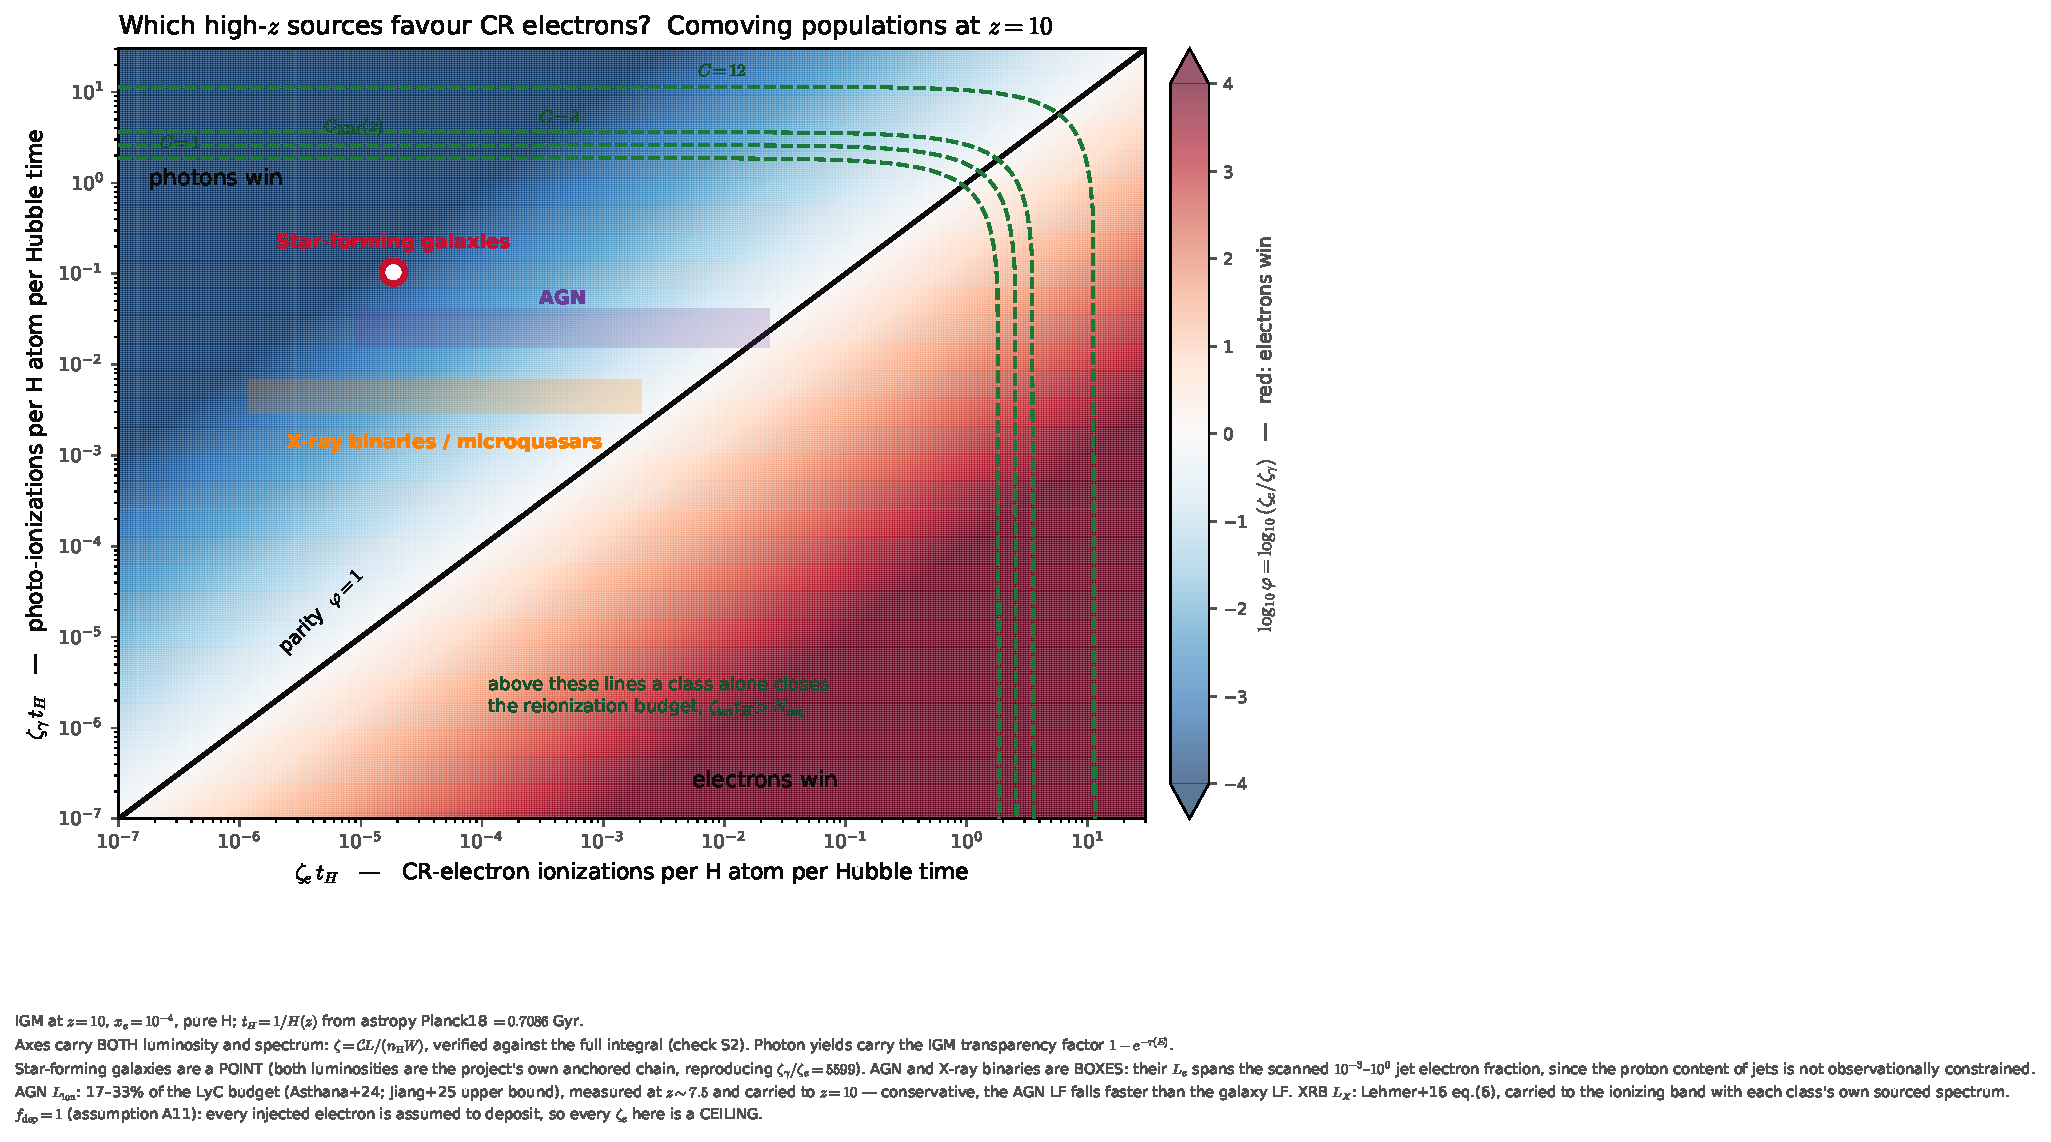
\includegraphics[width=0.86\textwidth]{source_budget_plane.pdf}
\caption{\textbf{The budget plane, comoving populations at $z=10$.}
Produced by \texttt{source\_map.py::make\_figure\_A}.}
\label{fig:budgetplane}
\end{figure}

\begin{figure}[p]\centering
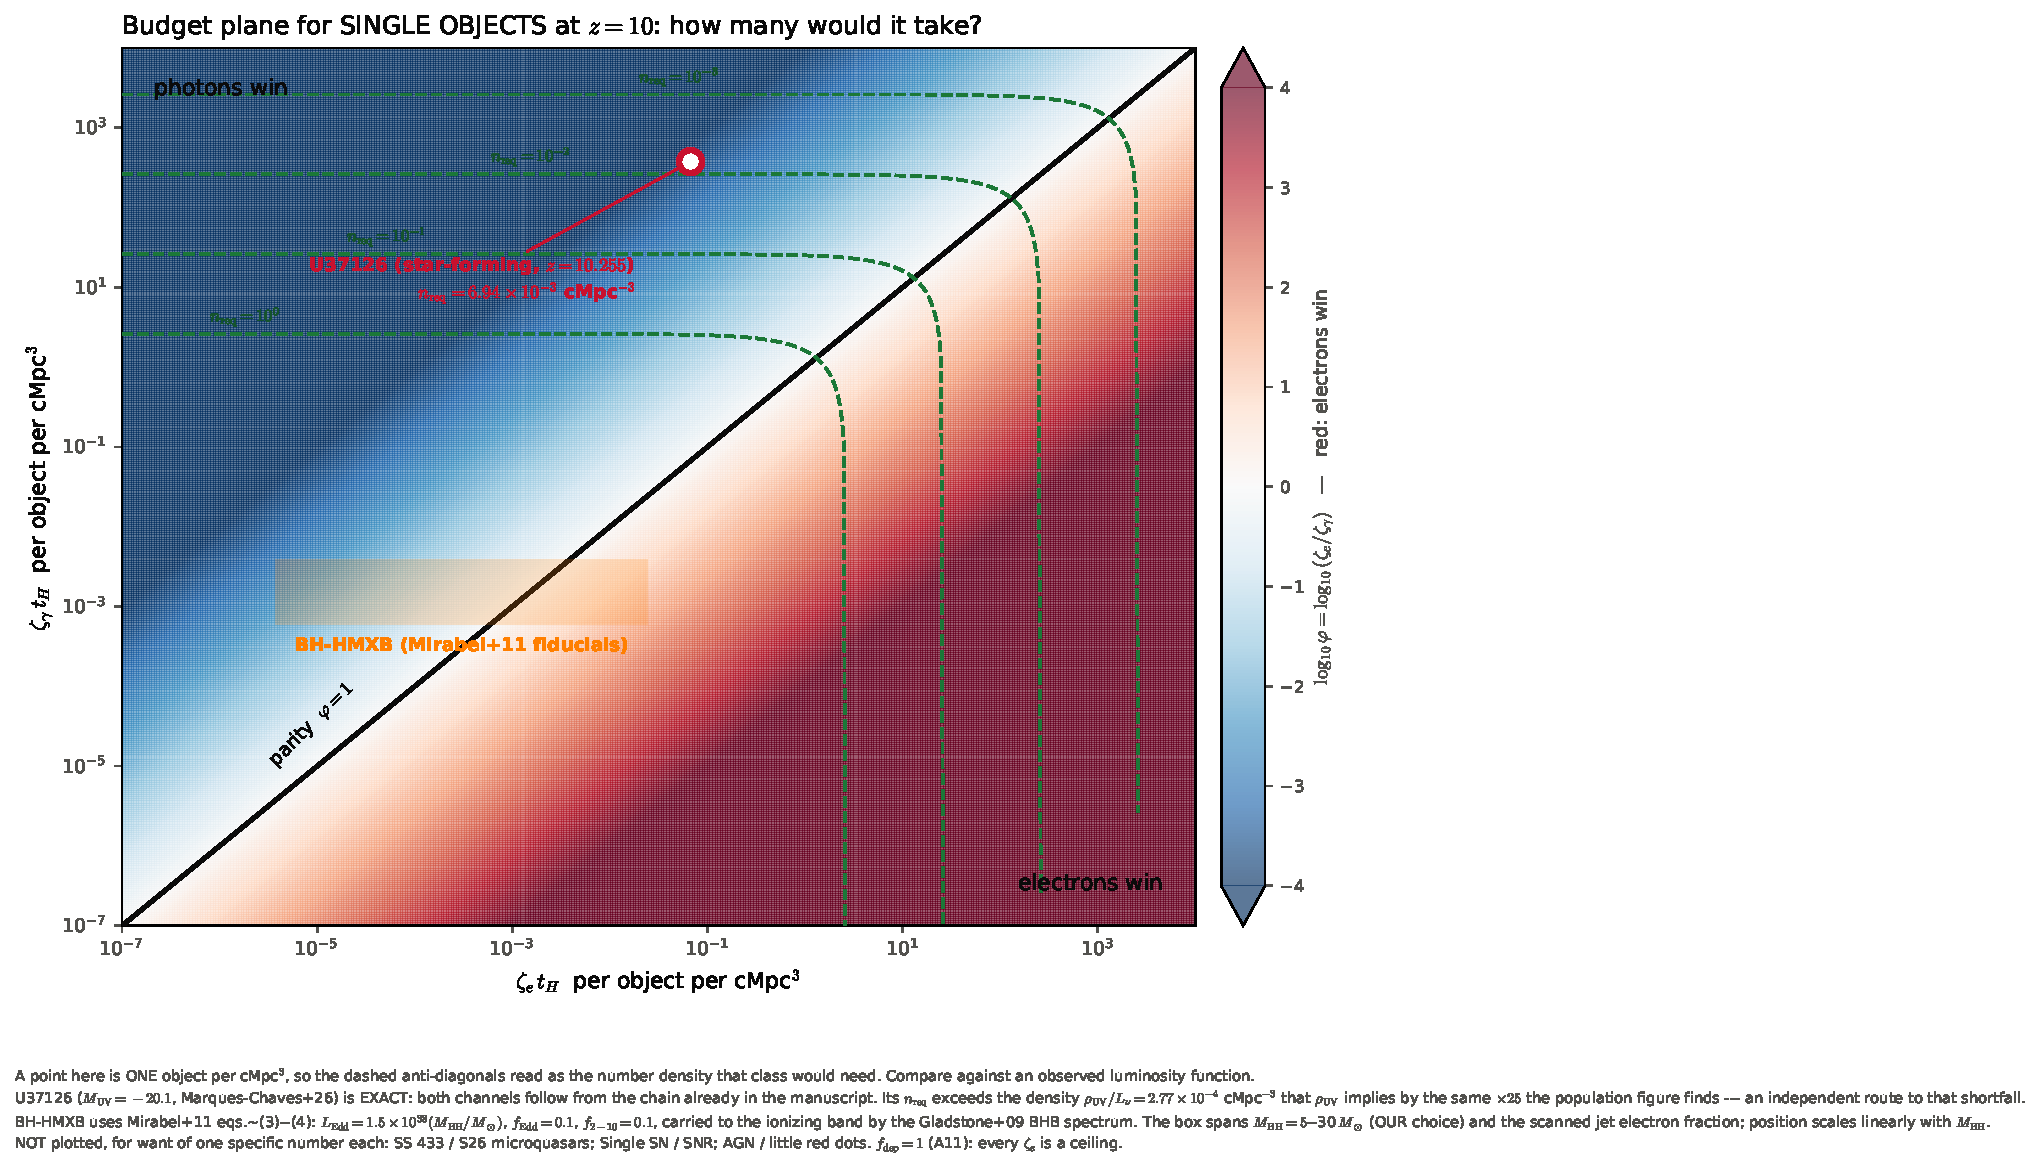
\includegraphics[width=0.86\textwidth]{source_budget_objects.pdf}
\caption{\textbf{The budget plane for single objects.} A point is one object per
cMpc$^3$, so the dashed anti-diagonals read as required number density.
Produced by \texttt{source\_map.py::make\_figure\_A\_objects}.}
\label{fig:budgetobjects}
\end{figure}

\begin{figure}[p]\centering
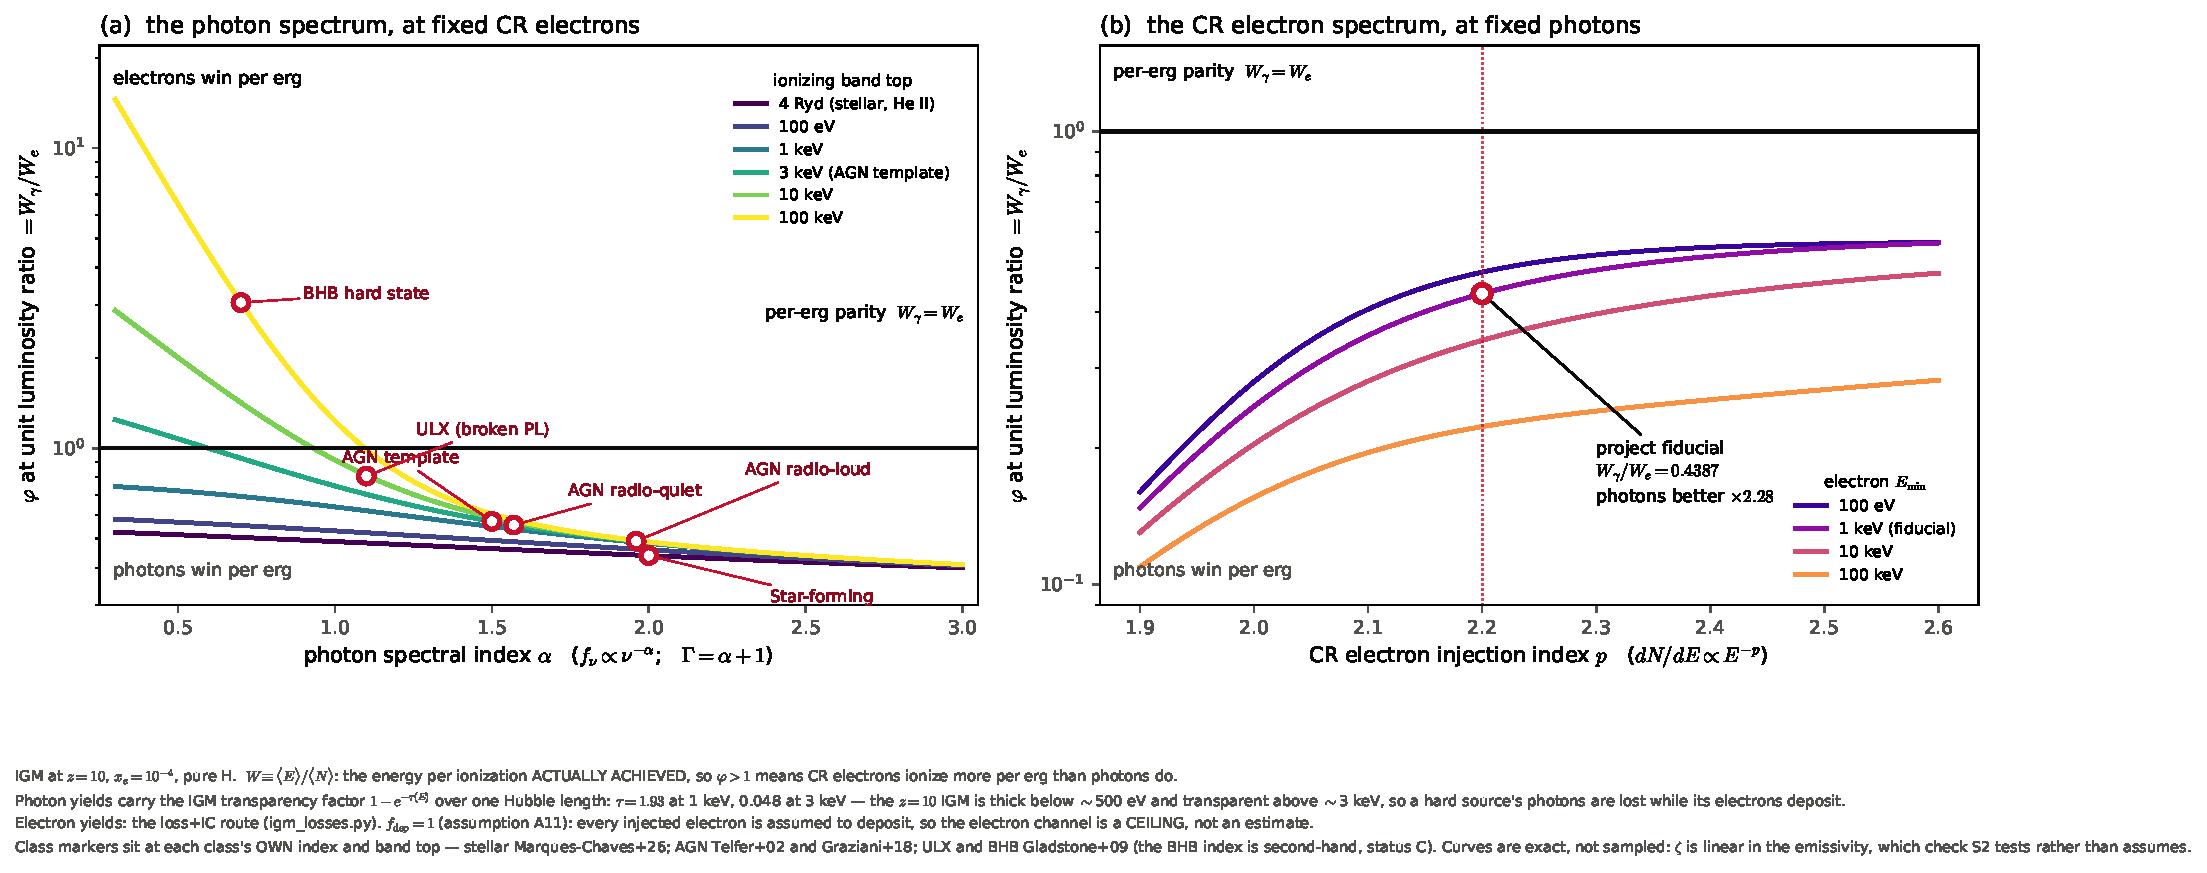
\includegraphics[width=\textwidth]{source_spectral_index.pdf}
\caption{\textbf{The spectral factor against each channel's index.}
Produced by \texttt{source\_map.py::make\_figure\_D}.}
\label{fig:spectralindex}
\end{figure}

\begin{figure}[p]\centering
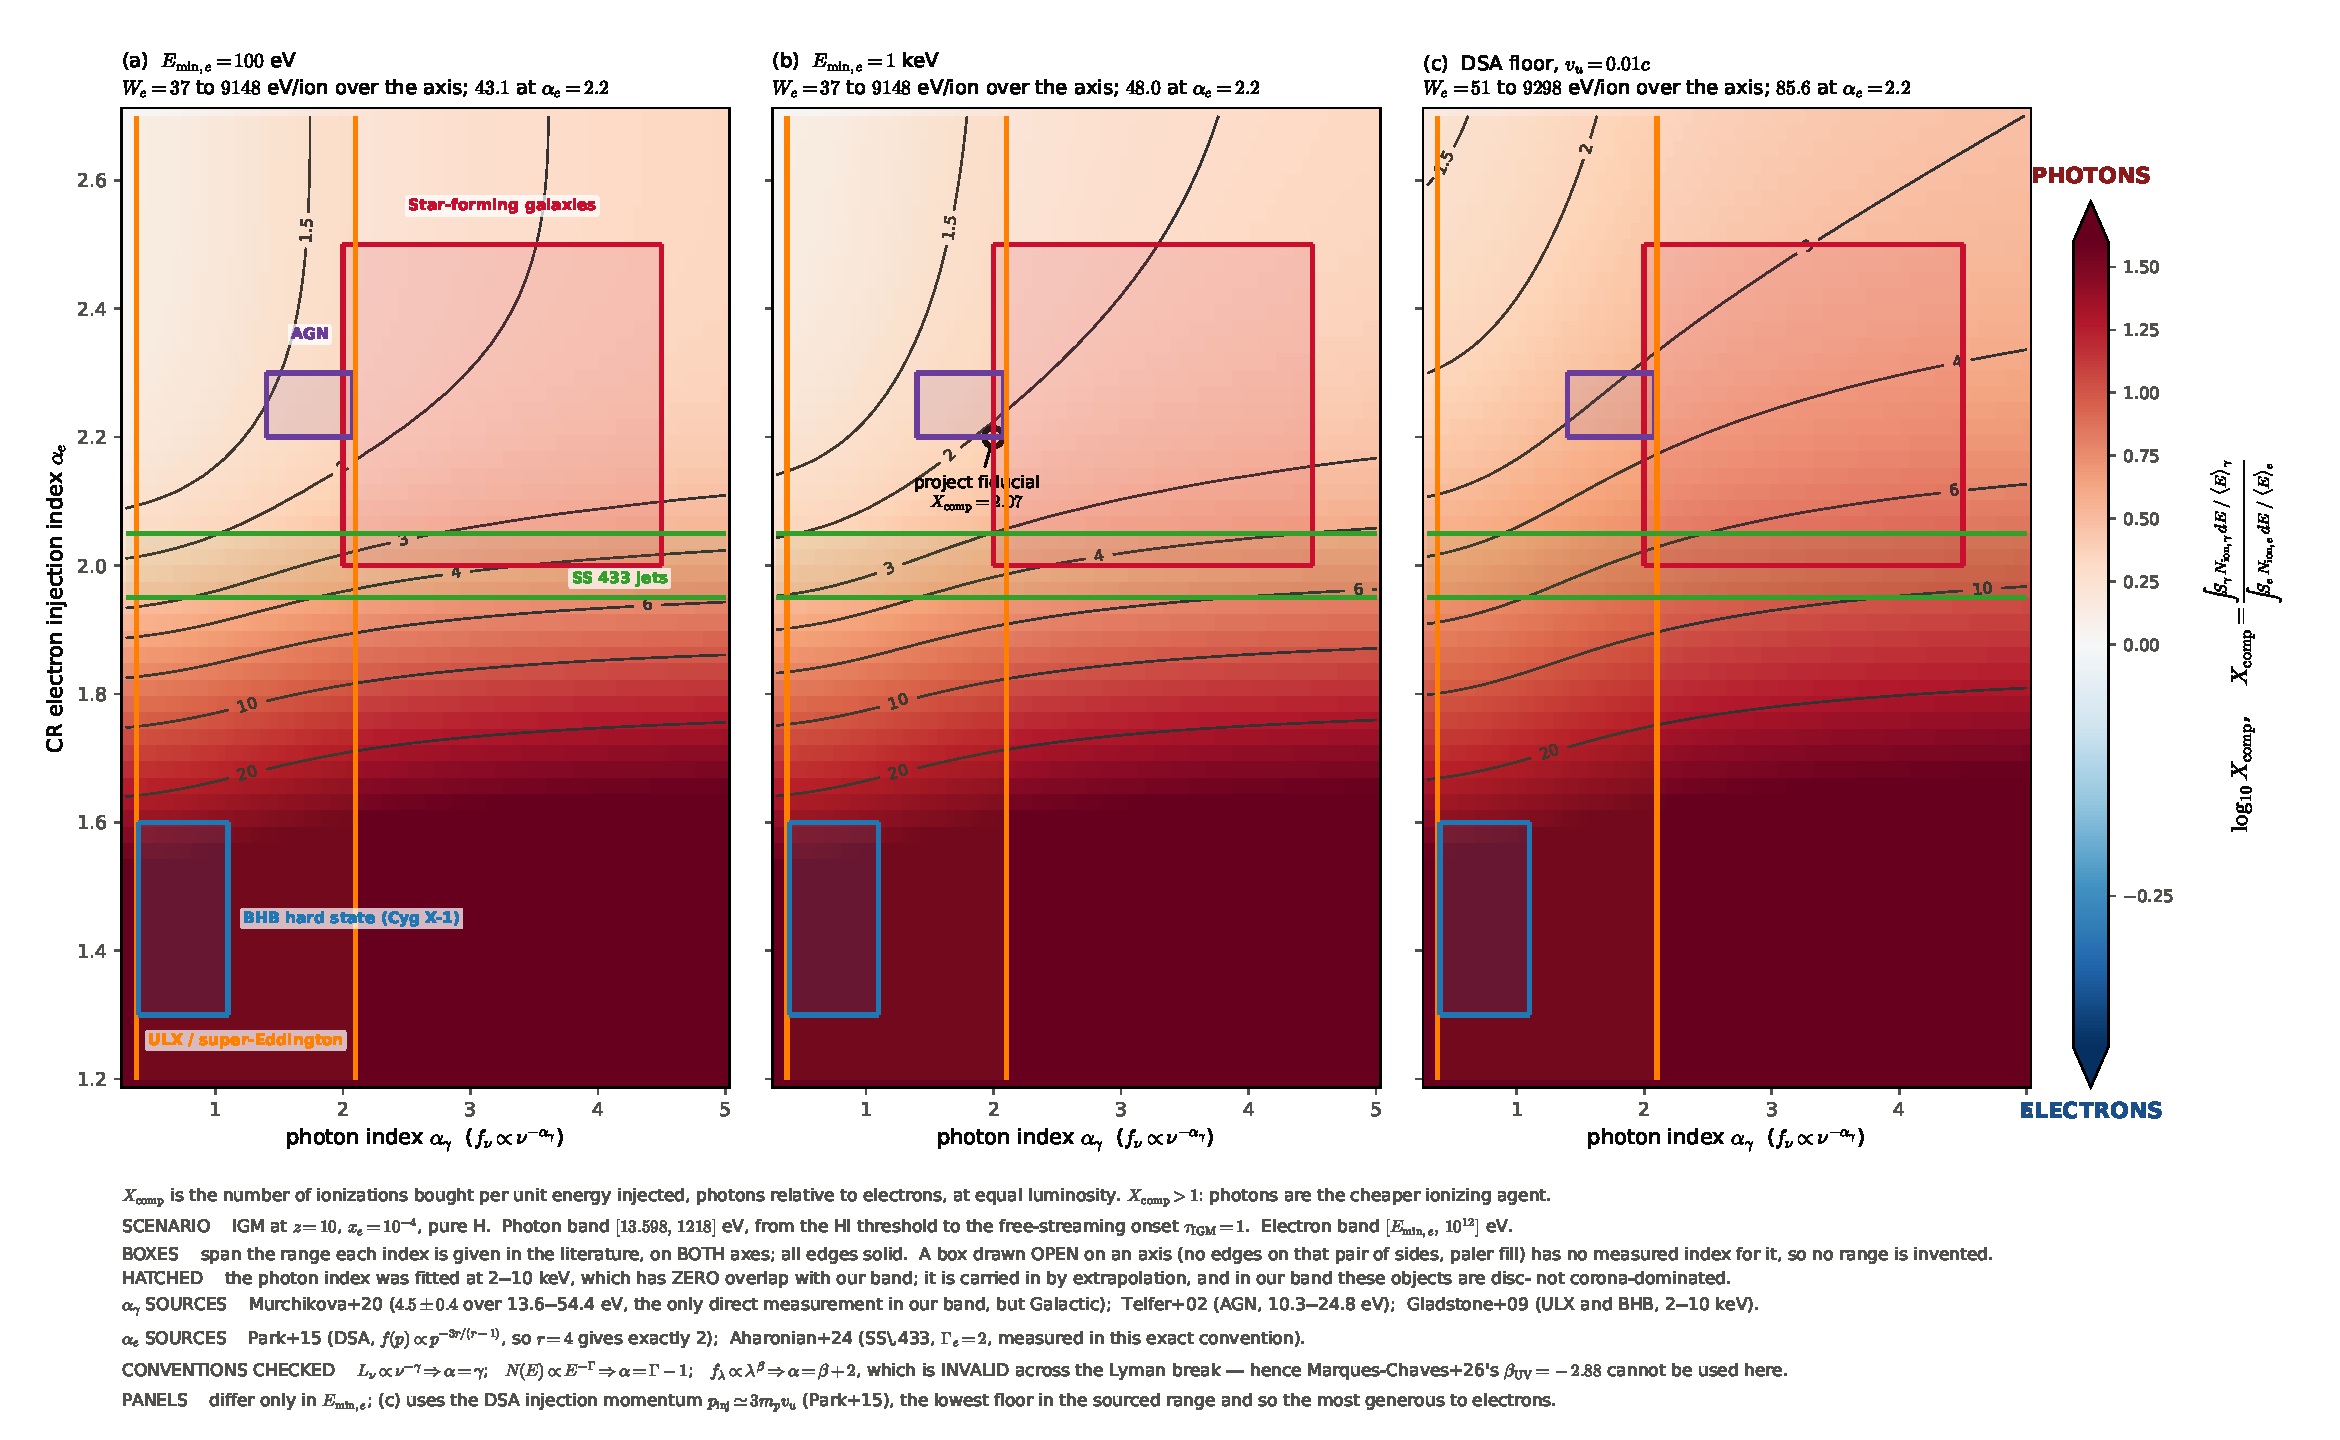
\includegraphics[width=\textwidth]{xcomp_map.pdf}
\caption{\textbf{$X_{\rm comp}$ over the two spectral indices}, at three electron
band floors. Produced by
\texttt{make\_xcomp\_definitions.py::make\_figure\_X}.}
\label{fig:xcompmap}
\end{figure}

\clearpage
\section{What was \emph{not} checked}\label{sec:notchecked}
\begin{enumerate}\itemsep2pt
\item \textbf{No independent reimplementation} (C24). Every cross-check but the
      agreement with \cite{leite17} is internal to this code and the companion.
\item \textbf{CR transport is ignored entirely} (assumption~10). Including escape
      or confinement can only weaken the CR channel, so the direction of the
      conclusion is safe; its magnitude is a lower bound on the gap.
\item \textbf{The LyC spectrum is a parametrised power law, not a solved
      stellar atmosphere.} It sets the shape of panel~(a); the totals depend on
      it only weakly because $\xi_{\rm ion}$ carries the normalisation
      (\S\ref{sec:sed}).
\item \textbf{Helium is absent} from the target, as in the companion work.
\item \textbf{$\zeta$ is not a reionization history}: no recombinations, no
      clumping, no radiative transfer, no spatial structure.
\end{enumerate}

\begin{thebibliography}{9}\small
\bibitem{donnan24} C.~T. Donnan et al., \emph{MNRAS} (2024), JWST PRIMER,
  arXiv:2403.03171. \emph{In the tree}: \texttt{papers/2403.03171-donnan-primer-uvlf.pdf}. Table 3.
\bibitem{llerena25} M.~Llerena et al., \emph{A\&A} \textbf{698}, A302 (2025), arXiv:2412.01358.
  \emph{In the tree}: \texttt{papers/2412.01358-llerena-xi-ion-z4-10.pdf}.
  $\log\xi_{\rm ion}=25.28$ is their median at $z\simeq7.14$; scatter $0.42$~dex.
\bibitem{md14} P.~Madau \& M.~Dickinson, \emph{ARA\&A} \textbf{52}, 415 (2014),
  arXiv:1403.0007. \emph{In the tree}:
  \texttt{papers/1403.0007-madau-dickinson-sfh-review.pdf}. $K_{\rm UV}=1.15\times10^{-28}$
  is their eq.~(10), quoted for a Salpeter IMF over $0.1$--$100\,M_\odot$ --- the same
  range this work integrates.
\bibitem{leite17} N.~Leite, C.~Evoli, M.~D'Angelo, B.~Ciardi, G.~Sigl \& A.~Ferrara,
  \emph{MNRAS} \textbf{469}, 416 (2017), arXiv:1703.09337. \emph{In the tree}:
  \texttt{papers/1703.09337-leite-cosmic-rays-heat-igm.pdf}.
\bibitem{ss15} S.~Sazonov \& R.~Sunyaev, \emph{MNRAS} \textbf{454}, 3464 (2015),
  arXiv:1509.08408. \emph{In the tree}:
  \texttt{papers/1509.08408-sazonov-sunyaev-cr-preheating.pdf}.
\bibitem{mc26} R.~Marques-Chaves et al., \emph{A\&A} (2026), arXiv:2602.02322.
  \emph{In the tree}: \texttt{papers/2602.02322-marques-chaves-u37126-z10.pdf}.
\bibitem{jeong25} T.~B. Jeong, M.~Jeon, H.~Song \& V.~Bromm,
  \emph{ApJ} (2025), arXiv:2411.17007. \emph{In the tree}:
  \texttt{papers/2411.17007-jeong-topheavy-imf-popII.pdf}. Eq.~(2): the
  top-heavy Pop~II IMF adopted here; \S5: the $\eta_{\rm UV}$ pair.
\bibitem{zackrisson11} E.~Zackrisson, C.-E. Rydberg, D.~Schaerer, G.~\"Ostlin
  \& M.~Tuli, \emph{ApJ} \textbf{740}, 13 (2011), arXiv:1105.0921.
  \emph{In the tree}: \texttt{papers/1105.0921-zackrisson-yggdrasil-2011.pdf}.
  Its IMFs are Kroupa (Pop~I/II), a log-normal $M_c=10\,M_\odot$ (Pop~III.2) and
  a Schaerer (2002) power law $\alpha=2.35$ over $50$--$500\,M_\odot$ at $Z=0$
  (Pop~III.1). It tabulates neither $\xi_{\rm ion}$ nor $K_{\rm UV}$.
\bibitem{larson98} R.~B. Larson, \emph{MNRAS} \textbf{301}, 569 (1998).
  \emph{Not in the tree}; the CMB temperature-floor argument for a rising
  characteristic mass at high $z$, cited through \cite{jeong25}.
\bibitem{of06} D.~E. Osterbrock \& G.~J. Ferland, \emph{Astrophysics of
  Gaseous Nebulae and Active Galactic Nuclei}, 2nd ed., University Science Books
  (2006). Table 2.1: case-B recombination coefficients for hydrogen.
\bibitem{hg97} L.~Hui \& N.~Y. Gnedin, \emph{MNRAS} \textbf{292}, 27 (1997),
  arXiv:astro-ph/9612232. \emph{In the tree}:
  \texttt{papers/astro-ph.9612232-hui-gnedin-1997-igm-eos.pdf}. The case-B
  $\alpha_B(T)$ fit used here to confirm the adopted value independently.
\bibitem{pawlik09} A.~H. Pawlik, J.~Schaye \& E.~van Scherpenzeel,
  \emph{MNRAS} \textbf{394}, 1812 (2009), arXiv:0807.3963. \emph{In the tree}:
  \texttt{papers/0807.3963-pawlik-schaye-clumping-factor.pdf}. Eq.~(A1) and
  Table~A1: the clumping-factor fit behind \cite{md14}'s $1+43z^{-1.71}$.
\bibitem{salpeter} E.~E. Salpeter, \emph{ApJ} \textbf{121}, 161 (1955).
  \emph{In the tree}: \texttt{papers/1955ApJ-121-161-salpeter-imf.pdf} (NASA ADS
  scanned article).
\bibitem{kim00} Y.-K. Kim, J.~P. Santos \& F. Parente, \emph{Phys. Rev. A} \textbf{62},
  052710 (2000), \texttt{doi:10.1103/PhysRevA.62.052710}.
  \emph{In the tree}: \texttt{papers/PhysRevA.62.052710-kim-santos-parente-2000-rbed.pdf}. Eq.~(20) is the RBED total
  cross section this work uses, eq.~(19) its differential form, eq.~(22) the RBEB
  variant it is \emph{not}. Verified against the code in \S\ref{sec:audit}.
\bibitem{kimrudd94} Y.-K. Kim \& M.~E. Rudd, \emph{Phys. Rev. A} \textbf{50}, 3954 (1994),
  \texttt{doi:10.1103/PhysRevA.50.3954}. \emph{In the tree}:
  \texttt{papers/PhysRevA.50.3954-kim-rudd-1994-bed.pdf}. Table~I supplies the H($1s$)
  $\mathrm{d}f/\mathrm{d}w$ coefficients, $B$, $U$, $M^2$ and $N_i$; eq.~(55) the
  BED total cross section, eq.~(56) $D(t)$.
\end{thebibliography}
\end{document}
